% Options for packages loaded elsewhere
\PassOptionsToPackage{unicode}{hyperref}
\PassOptionsToPackage{hyphens}{url}
%
\documentclass[
  11.5pt,
]{article}
\usepackage{amsmath,amssymb}
\usepackage{lmodern}
\usepackage{ifxetex,ifluatex}
\ifnum 0\ifxetex 1\fi\ifluatex 1\fi=0 % if pdftex
  \usepackage[T1]{fontenc}
  \usepackage[utf8]{inputenc}
  \usepackage{textcomp} % provide euro and other symbols
\else % if luatex or xetex
  \usepackage{unicode-math}
  \defaultfontfeatures{Scale=MatchLowercase}
  \defaultfontfeatures[\rmfamily]{Ligatures=TeX,Scale=1}
\fi
% Use upquote if available, for straight quotes in verbatim environments
\IfFileExists{upquote.sty}{\usepackage{upquote}}{}
\IfFileExists{microtype.sty}{% use microtype if available
  \usepackage[]{microtype}
  \UseMicrotypeSet[protrusion]{basicmath} % disable protrusion for tt fonts
}{}
\makeatletter
\@ifundefined{KOMAClassName}{% if non-KOMA class
  \IfFileExists{parskip.sty}{%
    \usepackage{parskip}
  }{% else
    \setlength{\parindent}{0pt}
    \setlength{\parskip}{6pt plus 2pt minus 1pt}}
}{% if KOMA class
  \KOMAoptions{parskip=half}}
\makeatother
\usepackage{xcolor}
\IfFileExists{xurl.sty}{\usepackage{xurl}}{} % add URL line breaks if available
\IfFileExists{bookmark.sty}{\usepackage{bookmark}}{\usepackage{hyperref}}
\hypersetup{
  hidelinks,
  pdfcreator={LaTeX via pandoc}}
\urlstyle{same} % disable monospaced font for URLs
\usepackage[margin=1in]{geometry}
\usepackage{graphicx}
\makeatletter
\def\maxwidth{\ifdim\Gin@nat@width>\linewidth\linewidth\else\Gin@nat@width\fi}
\def\maxheight{\ifdim\Gin@nat@height>\textheight\textheight\else\Gin@nat@height\fi}
\makeatother
% Scale images if necessary, so that they will not overflow the page
% margins by default, and it is still possible to overwrite the defaults
% using explicit options in \includegraphics[width, height, ...]{}
\setkeys{Gin}{width=\maxwidth,height=\maxheight,keepaspectratio}
% Set default figure placement to htbp
\makeatletter
\def\fps@figure{htbp}
\makeatother
\setlength{\emergencystretch}{3em} % prevent overfull lines
\providecommand{\tightlist}{%
  \setlength{\itemsep}{0pt}\setlength{\parskip}{0pt}}
\setcounter{secnumdepth}{5}
\usepackage{caption,booktabs,longtable,pdfpages,rotating,graphicx,footmisc,float,tikz,amsthm,afterpage,setspace,minitoc,appendix,etoc}
\captionsetup{width=5in}
\setlength\parindent{24pt}
\bibliographystyle{apsr}
\renewcommand{\footnotesize}{\fontsize{10pt}{10pt}\selectfont}
\renewcommand{\footnotelayout}{\setstretch{1.5}}
\setlength{\footnotesep}{\baselineskip}
\captionsetup{width=6in}
\renewcommand \thepart{}
\renewcommand \partname{}
\renewcommand{\thesection}{\Alph{section}}
\usepackage{lscape}
\newcommand{\blandscape}{\begin{landscape}}
\newcommand{\elandscape}{\end{landscape}}
\usepackage[margin=1in]{geometry}
\floatplacement{figure}{H}
\etocsettocstyle{\subsection*{\contentsname}}{\noindent\rule{\linewidth}{.4pt}}
\usepackage{booktabs}
\usepackage{longtable}
\usepackage{array}
\usepackage{multirow}
\usepackage{wrapfig}
\usepackage{float}
\usepackage{colortbl}
\usepackage{pdflscape}
\usepackage{tabu}
\usepackage{threeparttable}
\usepackage{threeparttablex}
\usepackage[normalem]{ulem}
\usepackage{makecell}
\usepackage{xcolor}
\ifluatex
  \usepackage{selnolig}  % disable illegal ligatures
\fi

\author{}
\date{\vspace{-2.5em}}

\begin{document}

\clearpage

\setcounter{page}{0}
\pagenumbering{arabic}
\setcounter{page}{1}

\part*{}

\begin{figure}
\centering
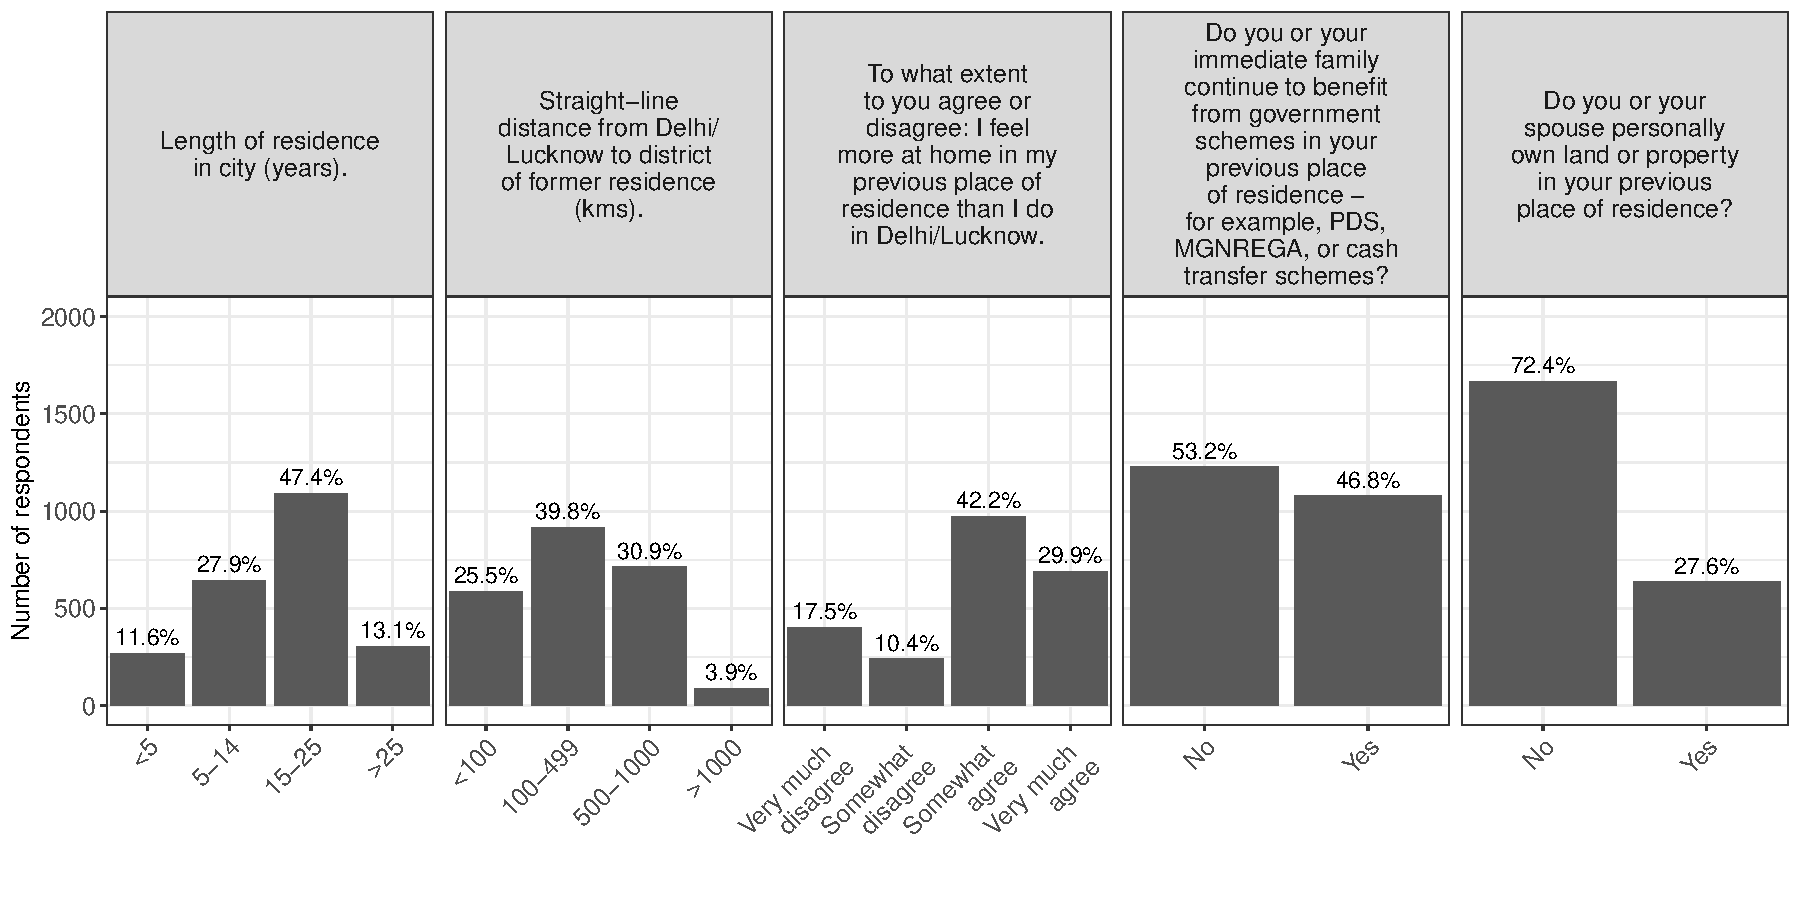
\includegraphics{supplementary-information_files/figure-latex/fig-1-1.pdf}
\caption{Baseline descriptive statistics of migants' attachments to
their former places of residence.}
\end{figure}

\clearpage

\begin{table}[!htbp] \centering 
  \caption{[Exploratory] Baseline correlates of migrants' continued political participation in their former place of residence (``hometown''), estimated using OLS regression. For question wordings, see Figure 1. Robust standard errors in parentheses.} 
  \label{} 
\small 
\begin{tabular}{@{\extracolsep{5pt}}lcc} 
\\[-1.8ex]\hline 
\hline \\[-1.8ex] 
 & \multicolumn{2}{c}{\textit{Dependent variable:}} \\ 
\cline{2-3} 
\\[-1.8ex] & Has Hometown Voter ID & Returned to Vote in Hometown \\ 
\\[-1.8ex] & (1) & (2)\\ 
\hline \\[-1.8ex] 
 More at home in hometown (0-1) & 0.158$^{***}$ & 0.088$^{***}$ \\ 
  & (0.025) & (0.020) \\ 
  Still receives hometown schemes (0/1) & 0.108$^{***}$ & 0.101$^{***}$ \\ 
  & (0.019) & (0.017) \\ 
  Owns hometown property (0/1) & 0.072$^{***}$ & 0.039$^{**}$ \\ 
  & (0.022) & (0.020) \\ 
  Length of residence in city (years) & $-$0.003$^{***}$ & $-$0.002$^{***}$ \\ 
  & (0.001) & (0.001) \\ 
  Straight-line distance to home district (kms) & $-$0.0001$^{**}$ & $-$0.0001$^{***}$ \\ 
  & (0.00003) & (0.00002) \\ 
  Constant & 0.177$^{***}$ & 0.146$^{***}$ \\ 
  & (0.027) & (0.022) \\ 
 \hline \\[-1.8ex] 
DV values & \{0,1\} & \{0,1\} \\ 
Observations & 2,306 & 2,306 \\ 
Adjusted R$^{2}$ & 0.056 & 0.047 \\ 
\hline 
\hline \\[-1.8ex] 
\multicolumn{3}{r}{$^{*}$p$<$0.1; $^{**}$p$<$0.05; $^{***}$p$<$0.01} \\ 
\end{tabular} 
\end{table}

\clearpage

\clearpage

\begin{table}

\caption{\label{tab:unnamed-chunk-8}[Pre-registered] T1 experimental results for primary political outcomes. Outcomes are whether respondent (1) currently has a voter ID card allowing them to vote in city elections; (2) voted in the city during the 2019 Lok Sabha elections; and (3) intends to vote in the next state elections held in the city. OLS estimates of intent to treat effects. Models include covariates. Robust standard errors in parentheses.}
\centering
\begin{tabular}[t]{lccc}
\toprule
 & \makecell[c]{Has City-Based\\ Voter ID \\(1)} & \makecell[c]{Voted in City\\ in 2019 \\(2)} & \makecell[c]{Likelihood of Voting\\ in City in Future \\(3)}\\
\midrule
T1 treatment & 0.236 & 0.203 & 0.031\\
 & (0.019) & (0.019) & (0.009)\\
\midrule
p-value (upper) & 0.000 & 0.000 & 0.000\\
Control mean & 0.161 & 0.178 & 0.856\\
Observations & 2,120 & 2,120 & 2,120\\
Adjusted $R^2$ & 0.084 & 0.065 & 0.011\\
DV values & $\{0, 1\}$ & $\{0, 1\}$ & $\{0, 0.33, 0.67, 1\}$\\
\bottomrule
\end{tabular}
\end{table}

\clearpage

\begin{table}

\caption{\label{tab:unnamed-chunk-9}[Pre-registered] T1 experimental results for additional political outcomes. Outcomes are whether respondent (1) pays attention to news about national, state, and city politics; (2) agrees that elected politicians are accountable to city residents; (3) agrees that citizens have an influence on the government; (4) has trust in the national, state, and city governments as well as political parties. OLS estimates of intent to treat effects. Models include covariates. Robust standard errors in parentheses.}
\centering
\begin{tabular}[t]{lcccc}
\toprule
 & \makecell[c]{Political\\ Interest\\ Index \\(1)} & \makecell[c]{Politician\\ Accountability\\ Perceptions \\(2)} & \makecell[c]{Sense of\\ Political\\ Efficacy \\(3)} & \makecell[c]{Political\\ Trust\\ Index \\(4)}\\
\midrule
T1 treatment & 0.091 & 0.039 & -0.012 & 0.027\\
 & (0.039) & (0.015) & (0.018) & (0.028)\\
\midrule
p-value (upper) & 0.010 & 0.003 & 0.745 & 0.170\\
Control mean & 0.000 & 0.697 & 0.450 & 0.000\\
Observations & 2,120 & 2,120 & 2,120 & 2,120\\
Adjusted $R^2$ & 0.027 & 0.006 & 0.003 & 0.019\\
DV values & $[-1.44, 1.56]$ & $\{0, 0.33, 0.67, 1\}$ & $\{0, 0.33, 0.67, 1\}$ & $[-1.62, 1.17]$\\
\bottomrule
\end{tabular}
\end{table}

\clearpage

\begin{table}[!htbp] \centering 
  \caption{[Pre-registered] Estimates of heterogeneous effects of T1 treatment. Models do not include additional covariates. All independent variables are dichotomous and are described in the text. Robust standard errors in parentheses.} 
  \label{} 
\small 
\begin{tabular}{@{\extracolsep{5pt}}lcc} 
\\[-1.8ex]\hline 
\hline \\[-1.8ex] 
 & \multicolumn{2}{c}{\textit{Dependent variable:}} \\ 
\cline{2-3} 
\\[-1.8ex] & Has City-Based Voter ID & Voted in City in 2019 \\ 
\\[-1.8ex] & (1) & (2)\\ 
\hline \\[-1.8ex] 
 T1 x Primary education & 0.083$^{**}$ & 0.057 \\ 
  & (0.041) & (0.042) \\ 
  T1 x Muslim & $-$0.114$^{**}$ & $-$0.018 \\ 
  & (0.048) & (0.049) \\ 
  T1 x SC/ST & $-$0.113$^{***}$ & $-$0.081$^{*}$ \\ 
  & (0.042) & (0.042) \\ 
  T1 x High income & 0.028 & 0.041 \\ 
  & (0.038) & (0.038) \\ 
  T1 x Long-term migrant & $-$0.019 & $-$0.007 \\ 
  & (0.038) & (0.038) \\ 
  T1 & 0.248$^{***}$ & 0.183$^{***}$ \\ 
  & (0.049) & (0.049) \\ 
  Primary education & $-$0.058$^{**}$ & $-$0.059$^{**}$ \\ 
  & (0.025) & (0.026) \\ 
  Muslim & 0.001 & 0.004 \\ 
  & (0.029) & (0.030) \\ 
  SC/ST & $-$0.004 & $-$0.008 \\ 
  & (0.025) & (0.026) \\ 
  High income & 0.038$^{*}$ & 0.009 \\ 
  & (0.022) & (0.023) \\ 
  Long-term migrant & 0.065$^{***}$ & 0.052$^{**}$ \\ 
  & (0.023) & (0.024) \\ 
  Constant & 0.149$^{***}$ & 0.188$^{***}$ \\ 
  & (0.028) & (0.029) \\ 
 \hline \\[-1.8ex] 
Observations & 2,120 & 2,120 \\ 
Adjusted R$^{2}$ & 0.087 & 0.059 \\ 
\hline 
\hline \\[-1.8ex] 
\multicolumn{3}{r}{$^{*}$p$<$0.1; $^{**}$p$<$0.05; $^{***}$p$<$0.01} \\ 
\end{tabular} 
\end{table}

\clearpage

\clearpage

\begin{table}

\caption{\label{tab:unnamed-chunk-12}[Index outcome pre-registered; index component analyses exploratory] T2 experimental results for exposure to campaigning during the 2019 Lok Sabha elections. Campaign exposure index (1) based on whether respondent reports that politicians or party workers (2) visited their basti around the 2019 Lok Sabha election campaign; (3) came to the door to request votes; (4) offered gifts; (5) tried to specifically win votes of recent migrants to the city; (6) campaigned hard to win votes in the basti. Weighted least squares estimates of intent to treat effects. Clusters weighted equally. Models include block fixed effects and individual covariates. Cluster-robust standard errors in parentheses.}
\centering
\fontsize{10}{12}\selectfont
\begin{tabular}[t]{lcccccc}
\toprule
\multicolumn{1}{c}{} & \multicolumn{1}{c}{ } & \multicolumn{5}{c}{Index Components} \\
\cmidrule(l{3pt}r{3pt}){3-7}
 & \makecell[c]{Campaigning\\ Exposure\\ Index \\(1)} & \makecell[c]{Basti\\Visits by\\ Politicians \\(2)} & \makecell[c]{Home Visit\\ by Politician or\\ Party Worker  \\(3)} & \makecell[c]{Number\\ of\\ Gifts \\(4)} & \makecell[c]{Migrant-\\ Focused\\ Campaigning \\(5)} & \makecell[c]{Perceived\\ Campaign\\ Intensity \\(6)}\\
\midrule
T2 treatment & 0.101 & 0.066 & 0.036 & 0.017 & 0.014 & 0.073\\
 & (0.058) & (0.078) & (0.038) & (0.012) & (0.047) & (0.031)\\
\midrule
p-value (upper) & 0.043 & 0.203 & 0.174 & 0.073 & 0.384 & 0.010\\
Control mean & -0.039 & 0.559 & 0.550 & 0.013 & 0.425 & 0.676\\
Observations & 1,969 & 1,969 & 1,969 & 1,969 & 1,969 & 1,931\\
No. of Clusters & 87 & 87 & 87 & 87 & 87 & 87\\
Adjusted $R^2$ & 0.056 & 0.070 & 0.047 & 0.019 & 0.008 & 0.021\\
DV values & $[-0.96, 3.65]$ & $\{0, \ldots, 4\}$ & $\{0, 1\}$ & $\{0, 1, 2\}$ & $\{0, 1\}$ & $\{0, 0.33, 0.67, 1\}$\\
\bottomrule
\end{tabular}
\end{table}

\clearpage

\begin{center}
\Large{\textbf{Overcoming the Political Exclusion of Migrants: Theory and Experimental Evidence from India}}
\end{center}

\vspace{20pt}

\begin{center}
\large{\textbf{Nikhar Gaikwad, Columbia University}}
\end{center}

\begin{center}
\large{\textbf{Gareth Nellis, University of California, San Diego}}
\end{center}

\vspace{20pt}

\begin{center}
\huge{ONLINE APPENDIX}
\end{center}

\vspace{20pt}

\begin{center}
\huge{\textit{Note: All references to ``Supplementary Information'' (``SI'') relate to the document, supplementary-information.pdf available at: https://doi.org/10.7910/DVN/G1JCKK}}
\end{center}

\setcounter{page}{0}
\pagenumbering{arabic}
\setcounter{page}{1}
\setcounter{figure}{0}
\setcounter{table}{0}
\renewcommand{\thefigure}{A\arabic{figure}}
\renewcommand{\thetable}{A\arabic{table}}

\clearpage

\part*{Online Appendix}
\addcontentsline{toc}{part}{Online Appendix}
\localtableofcontents

\clearpage

\section{Voter turnout rates among naturalized immigrants versus native-born citizens globally}

\begin{table}[!h]

\caption{\label{tab:unnamed-chunk-13}Average voter turnout rates by natives versus naturalized immigrants, according to the sixth wave of the World Values Survey (2010-14). Turnout percentages are calculated using data from all countries where responses to two questions were gathered: ``Respondent immigrant?'' (1 = yes; 0 = no), and ``Vote in elections?'' (1 = always/usually; 0 otherwise). Included countries are: Algeria, Azerbaijan, Argentina, Armenia, Brazil, Belarus, Chile, Taiwan, Colombia, Cyprus, Estonia, Georgia, Germany, Ghana, Haiti, India, Iraq, Kazakhstan, Jordan, South Korea, Kyrgyzstan, Lebanon, Libya, Malaysia, Mexico, Morocco, Netherlands, New Zealand, Nigeria, Pakistan, Peru, Philippines, Poland, Qatar, Romania, Russia, Rwanda, Singapore, Slovenia, South Africa, Zimbabwe, Sweden, Thailand, Trinidad and Tobago, Tunisia, Turkey, Ukraine, Egypt, United States, Uruguay, Uzbekistan, and Yemen.}
\centering
\resizebox{\linewidth}{!}{
\fontsize{12}{14}\selectfont
\begin{tabular}[t]{>{\raggedright\arraybackslash}p{20em}>{\raggedright\arraybackslash}p{20em}}
\toprule
Native turnout percent & Naturalized immigrant turnout percent\\
\midrule
81.82 & 71.1\\
\bottomrule
\end{tabular}}
\end{table}

\section{Indian Human Development Survey-II analysis}

In this section we characterize India's migrant population using
nationally representative survey data. We do this to shed light on the
political behaviors of migrants versus non-migrants, and to assess the
extent to which our sample conforms to---or deviates from---the
demographic traits of the country's migrant population at large.

Our primary resource for conducting these analyses is the second round
of the Indian Human Development Survey (IHDS-II). To our knowledge,
IHDS-II is unique among nationally representative surveys in posing both
detailed questions about respondents' migration history and asking a
battery of questions about political participation. Table
\ref{tab:ihds2_variables} gives a full roster of the IHDS-II variables
used in the subsequent analyses and notes the manner in which they were
recoded, where appropriate.

Note, in what follows, we decompose the IHDS-II sample into rural and
urban areas for the purposes of most analysis (according to the primary
sampling unit's designation given in the 2011 Census of India). This is
based on the presumption that rural areas are overwhelmingly
migrant-\textit{sending} regions whereas urban areas are largely
migrant-\textit{receiving} regions. In rural areas, we examine
differences between households that did and did not report having had a
member who engaged in seasonal migration during the past five years (a
question directly posed on the survey). In urban areas, defining who is
a migrant is more complex. Respondents were asked about the migration
history of their ``families'' and when their family first came to their
current town or city of residence. We class as internal migrants those
reporting that their families arrived from a different Indian district
or state within the past 10 years.

\subsection{Political participation}

Turning to the substantive analysis, we first investigate whether
migrants and migrant-sending households participate less in politics
than non-migrants. We generate a Political Engagement Index, which sums
whether (a) the household respondent reported being a member of a
political party, (b) a member of the village panchayat (in rural areas)
or ward committee (in urban areas), and (c) whether they reported having
attended a panchayat or ward committee meeting within the last year.

For both urban (Table \ref{tab:ihds2_political_engagement_urban}) and
rural (Table \ref{tab:ihds2_political_engagement_rural}) samples, we
find strong evidence that migrants and migrant-sending households,
respectively, are less likely to be politically engaged than households
not involved in migration.

In Table \ref{tab:ihds2_ses}, we demonstrate in the pooled (rural and
urban) data that the migrant/non-migrant participation gap persists
after controlling for households' religious affiliation.

While IHDS-II does not ask directly about voting, this analysis
significantly adds to the body of evidence suggesting that India's
internal migrants are politically disempowered.

\begin{table}[!htbp] \centering 
  \caption{[Exploratory] Are migrant households less politically engaged than non-migrant households in urban areas? Data are from the IHDS-II household-level recode file. Robust standard errors in parentheses.} 
  \label{tab:ihds2_political_engagement_urban} 
\small 
\begin{tabular}{@{\extracolsep{5pt}}lcccc} 
\\[-1.8ex]\hline 
\hline \\[-1.8ex] 
 & \multicolumn{4}{c}{\textit{Dependent variable:}} \\ 
\cline{2-5} 
\\[-1.8ex] & \shortstack{Political \\ Engagement \\ Index} & \shortstack{Political \\ Party \\ Member} & \shortstack{Ward \\ Committee \\ Member} & \shortstack{Attended \\ Ward Committee \\ Meeting} \\ 
\\[-1.8ex] & (1) & (2) & (3) & (4)\\ 
\hline \\[-1.8ex] 
 Migrant & $-$0.039$^{***}$ & $-$0.035$^{***}$ & $-$0.007 & $-$0.077$^{***}$ \\ 
  & (0.007) & (0.006) & (0.008) & (0.017) \\ 
  Constant & 0.073$^{***}$ & 0.042$^{***}$ & 0.022$^{***}$ & 0.154$^{***}$ \\ 
  & (0.001) & (0.002) & (0.001) & (0.003) \\ 
 \hline \\[-1.8ex] 
Observations & 14,500 & 14,546 & 14,504 & 14,516 \\ 
Adjusted R$^{2}$ & 0.001 & 0.0005 & $-$0.00003 & 0.001 \\ 
\hline 
\hline \\[-1.8ex] 
\multicolumn{5}{r}{$^{*}$p$<$0.1; $^{**}$p$<$0.05; $^{***}$p$<$0.01} \\ 
\end{tabular} 
\end{table}

\begin{table}[!htbp] \centering 
  \caption{[Exploratory] Are migrant-sending households less politically engaged than non-migrant-sending households in rural areas? Data are from the IHDS-II household-level recode file. Robust standard errors in parentheses.} 
  \label{tab:ihds2_political_engagement_rural} 
\small 
\begin{tabular}{@{\extracolsep{5pt}}lcccc} 
\\[-1.8ex]\hline 
\hline \\[-1.8ex] 
 & \multicolumn{4}{c}{\textit{Dependent variable:}} \\ 
\cline{2-5} 
\\[-1.8ex] & \shortstack{Political \\ Engagement \\ Index} & \shortstack{Political \\ Party \\ Member} & \shortstack{Panchayat \\ Member} & \shortstack{Attended \\ Panchayat \\ Meeting} \\ 
\\[-1.8ex] & (1) & (2) & (3) & (4)\\ 
\hline \\[-1.8ex] 
 \shortstack{Migrant-sending \\ household} & $-$0.010$^{**}$ & $-$0.013$^{***}$ & $-$0.015$^{***}$ & $-$0.002 \\ 
  & (0.004) & (0.003) & (0.004) & (0.010) \\ 
  Constant & 0.153$^{***}$ & 0.037$^{***}$ & 0.052$^{***}$ & 0.370$^{***}$ \\ 
  & (0.001) & (0.001) & (0.001) & (0.003) \\ 
 \hline \\[-1.8ex] 
Observations & 26,936 & 27,040 & 26,948 & 26,989 \\ 
Adjusted R$^{2}$ & 0.0001 & 0.0004 & 0.0003 & $-$0.00004 \\ 
\hline 
\hline \\[-1.8ex] 
\multicolumn{5}{r}{$^{*}$p$<$0.1; $^{**}$p$<$0.05; $^{***}$p$<$0.01} \\ 
\end{tabular} 
\end{table}

\begin{table}[!htbp] \centering 
  \caption{[Exploratory] Are migrant and migrant-sending households less politically engaged than non-migrant households after controlling for religion? Data are from the IHDS-II household-level recode file. Urban and rural samples are pooled. Robust standard errors in parentheses.} 
  \label{tab:ihds2_ses} 
\small 
\begin{tabular}{@{\extracolsep{5pt}}lc} 
\\[-1.8ex]\hline 
\hline \\[-1.8ex] 
 & \multicolumn{1}{c}{\textit{Dependent variable:}} \\ 
\cline{2-2} 
\\[-1.8ex] & \shortstack{Political \\ Engagement \\ Index} \\ 
\hline \\[-1.8ex] 
 Migrant/migrant-sending household & $-$0.013$^{***}$ \\ 
  & (0.004) \\ 
  Muslim & $-$0.020$^{***}$ \\ 
  & (0.003) \\ 
  Urban & $-$0.080$^{***}$ \\ 
  & (0.002) \\ 
  Constant & 0.156$^{***}$ \\ 
  & (0.001) \\ 
 \hline \\[-1.8ex] 
Observations & 41,436 \\ 
Adjusted R$^{2}$ & 0.038 \\ 
\hline 
\hline \\[-1.8ex] 
\multicolumn{2}{r}{$^{*}$p$<$0.1; $^{**}$p$<$0.05; $^{***}$p$<$0.01} \\ 
\end{tabular} 
\end{table}

\clearpage

\subsection{Politician attachments and receipt of government benefits}

We next turn to evaluate the extent to which migrants (in urban areas)
and migrant-sending households (in rural areas) are embedded in networks
of clientelistic exchange operated by local politicians. To be sure,
measuring quid pro quo transactions of material benefits for votes is
challenging. To understand how likely it is that households are involved
in such transactions, we make use of two sets of questions put to
respondents in the IHDS-II survey instrument: acquaintance with local
politicians, and income received from government schemes. Our reasoning
is that households who are not acquainted with local politicians are
unlikely to be able to access state benefits via clientelistic
mechanisms, and, from another angle, that those not receiving
substantial income from government schemes are unlikely to be involved
in a substantial votes-for-benefits exchange relationship with local
politicians, who have significant sway over how state resources are
allocated. The Acquaintance Index is the average of the four component
binary acquaintance measures.

In Tables \ref{tab:ihds2_acquaintance_urban} we observe that migrants in
urban India are similarly acquainted with local politicians as are
non-migrants, while Table \ref{tab:ihds2_benefits_income_urban}
demonstrates that urban migrants are significantly less likely to
receive income from state-run schemes.

\begin{table}[!htbp] \centering 
  \caption{[Exploratory] Are migrant households less connected to politicians than non-migrant households in urban areas? Data are from the IHDS-II household-level recode file. Robust standard errors in parentheses.} 
  \label{tab:ihds2_acquaintance_urban} 
\fontsize{10pt}{10pt}\selectfont
\begin{tabular}{@{\extracolsep{5pt}}lccccc} 
\\[-1.8ex]\hline 
\hline \\[-1.8ex] 
 & \multicolumn{5}{c}{\textit{Dependent variable:}} \\ 
\cline{2-6} 
\\[-1.8ex] & \shortstack{Acquaintance \\ Index} & \shortstack{Acquaintance: \\ Politician in \\ Community} & \shortstack{Acquaintance: \\ Politician \\ Outside \\ Community} & \shortstack{Acquaintance: \\ Party Worker \\ in Community} & \shortstack{Acquaintance: \\ Party Worker \\ Outside \\ Community} \\ 
\\[-1.8ex] & (1) & (2) & (3) & (4) & (5)\\ 
\hline \\[-1.8ex] 
 Migrant & 0.0005 & 0.001 & 0.004 & 0.004 & $-$0.008 \\ 
  & (0.017) & (0.016) & (0.022) & (0.019) & (0.022) \\ 
  Constant & 0.118$^{***}$ & 0.068$^{***}$ & 0.145$^{***}$ & 0.104$^{***}$ & 0.158$^{***}$ \\ 
  & (0.002) & (0.002) & (0.003) & (0.003) & (0.003) \\ 
 \hline \\[-1.8ex] 
Observations & 14,458 & 14,533 & 14,496 & 14,509 & 14,470 \\ 
Adjusted R$^{2}$ & $-$0.0001 & $-$0.0001 & $-$0.0001 & $-$0.0001 & $-$0.0001 \\ 
\hline 
\hline \\[-1.8ex] 
\multicolumn{6}{r}{$^{*}$p$<$0.1; $^{**}$p$<$0.05; $^{***}$p$<$0.01} \\ 
\end{tabular} 
\end{table}

\begin{table}[!htbp] \centering 
  \caption{[Exploratory] Do migrant households receive less income from government schemes than non-migrant households in urban areas? Data are from the IHDS-II household-level recode file. Robust standard errors in parentheses.} 
  \label{tab:ihds2_benefits_income_urban} 
\small 
\begin{tabular}{@{\extracolsep{5pt}}lc} 
\\[-1.8ex]\hline 
\hline \\[-1.8ex] 
 & \multicolumn{1}{c}{\textit{Dependent variable:}} \\ 
\cline{2-2} 
\\[-1.8ex] & Winsorized Benefits Income \\ 
\hline \\[-1.8ex] 
 Migrant & $-$272.713$^{***}$ \\ 
  & (80.823) \\ 
  Constant & 659.872$^{***}$ \\ 
  & (13.059) \\ 
 \hline \\[-1.8ex] 
Observations & 14,572 \\ 
Adjusted R$^{2}$ & 0.0005 \\ 
\hline 
\hline \\[-1.8ex] 
\multicolumn{2}{r}{$^{*}$p$<$0.1; $^{**}$p$<$0.05; $^{***}$p$<$0.01} \\ 
\end{tabular} 
\end{table}

Looking at the rural sample, Table \ref{tab:ihds2_acquaintance_rural}
shows that migrant-sending households are substantially less likely to
have connections with local politicians by comparison with other
households. They also receive somewhat less in income from government
schemes (see Table \ref{tab:ihds2_benefits_income_rural}).

\begin{table}[!htbp] \centering 
  \caption{[Exploratory] Are migrant-sending households less connected to politicians than non-migrant-sending households in rural areas? Data are from the IHDS-II household-level recode file. Robust standard errors in parentheses.} 
  \label{tab:ihds2_acquaintance_rural} 
\fontsize{10pt}{10pt}\selectfont
\begin{tabular}{@{\extracolsep{5pt}}lccccc} 
\\[-1.8ex]\hline 
\hline \\[-1.8ex] 
 & \multicolumn{5}{c}{\textit{Dependent variable:}} \\ 
\cline{2-6} 
\\[-1.8ex] & \shortstack{Acquaintance \\ Index} & \shortstack{Acquaintance: \\ Politician in \\ Community} & \shortstack{Acquaintance: \\ Politician \\ Outside \\ Community} & \shortstack{Acquaintance: \\ Party Worker \\ in Community} & \shortstack{Acquaintance: \\ Party Worker \\ Outside \\ Community} \\ 
\\[-1.8ex] & (1) & (2) & (3) & (4) & (5)\\ 
\hline \\[-1.8ex] 
 \shortstack{Migrant-sending \\ household} & $-$0.034$^{***}$ & $-$0.024$^{***}$ & $-$0.043$^{***}$ & $-$0.020$^{***}$ & $-$0.046$^{***}$ \\ 
  & (0.003) & (0.004) & (0.006) & (0.004) & (0.006) \\ 
  Constant & 0.093$^{***}$ & 0.066$^{***}$ & 0.127$^{***}$ & 0.063$^{***}$ & 0.115$^{***}$ \\ 
  & (0.001) & (0.002) & (0.002) & (0.002) & (0.002) \\ 
 \hline \\[-1.8ex] 
Observations & 26,924 & 27,026 & 26,965 & 26,996 & 26,931 \\ 
Adjusted R$^{2}$ & 0.002 & 0.001 & 0.001 & 0.001 & 0.002 \\ 
\hline 
\hline \\[-1.8ex] 
\multicolumn{6}{r}{$^{*}$p$<$0.1; $^{**}$p$<$0.05; $^{***}$p$<$0.01} \\ 
\end{tabular} 
\end{table}

\begin{table}[!htbp] \centering 
  \caption{[Exploratory] Do migrant-sending households receive less income from government schemes than non-migrant-sending households in rural areas? Data are from the IHDS-II household-level recode file. Robust standard errors in parentheses.} 
  \label{tab:ihds2_benefits_income_rural} 
\small 
\begin{tabular}{@{\extracolsep{5pt}}lc} 
\\[-1.8ex]\hline 
\hline \\[-1.8ex] 
 & \multicolumn{1}{c}{\textit{Dependent variable:}} \\ 
\cline{2-2} 
\\[-1.8ex] & Winsorized Benefits Income \\ 
\hline \\[-1.8ex] 
 \shortstack{Migrant-sending \\ household} & $-$60.649$^{*}$ \\ 
  & (34.996) \\ 
  Constant & 1,048.111$^{***}$ \\ 
  & (11.611) \\ 
 \hline \\[-1.8ex] 
Observations & 27,080 \\ 
Adjusted R$^{2}$ & 0.0001 \\ 
\hline 
\hline \\[-1.8ex] 
\multicolumn{2}{r}{$^{*}$p$<$0.1; $^{**}$p$<$0.05; $^{***}$p$<$0.01} \\ 
\end{tabular} 
\end{table}

\subsection{Confidence in political institutions}

IHDS-II respondents were asked about their confidence in various
political institutions. We see that migrant households in urban areas
(Table \ref{tab:ihds2_confidence_urban}) and migrant-sending households
in rural areas (Table \ref{tab:ihds2_confidence_rural}) express less
confidence in major political institutions than households not involved
in migration. In what follows, the Confidence Index is the average of
the three component confidence measures.

\begin{table}[!htbp] \centering 
  \caption{[Exploratory] Do migrant households express less confidence in political institutions than non-migrant households in urban areas? Data are from the IHDS-II household-level recode file. Robust standard errors in parentheses.} 
  \label{tab:ihds2_confidence_urban} 
\small 
\begin{tabular}{@{\extracolsep{5pt}}lcccc} 
\\[-1.8ex]\hline 
\hline \\[-1.8ex] 
 & \multicolumn{4}{c}{\textit{Dependent variable:}} \\ 
\cline{2-5} 
\\[-1.8ex] & \shortstack{Confidence \\ Index} & \shortstack{Confidence: \\ Ward Committees} & \shortstack{Confidence: \\ Politicians} & \shortstack{Confidence: \\ State Government} \\ 
\\[-1.8ex] & (1) & (2) & (3) & (4)\\ 
\hline \\[-1.8ex] 
 Migrant & $-$0.034$^{**}$ & $-$0.122$^{***}$ & $-$0.016 & $-$0.069 \\ 
  & (0.016) & (0.042) & (0.040) & (0.044) \\ 
  Constant & 0.447$^{***}$ & 1.046$^{***}$ & 0.577$^{***}$ & 1.061$^{***}$ \\ 
  & (0.002) & (0.006) & (0.005) & (0.006) \\ 
 \hline \\[-1.8ex] 
Observations & 14,467 & 14,517 & 14,536 & 14,482 \\ 
Adjusted R$^{2}$ & 0.0003 & 0.001 & $-$0.0001 & 0.0001 \\ 
\hline 
\hline \\[-1.8ex] 
\multicolumn{5}{r}{$^{*}$p$<$0.1; $^{**}$p$<$0.05; $^{***}$p$<$0.01} \\ 
\end{tabular} 
\end{table}

\begin{table}[!htbp] \centering 
  \caption{[Exploratory] Do migrant-sending households express less confidence in political institutions than non-migrant-sending households in rural areas? Data are from the IHDS-II household-level recode file. Robust standard errors in parentheses.} 
  \label{tab:ihds2_confidence_rural} 
\small 
\begin{tabular}{@{\extracolsep{5pt}}lcccc} 
\\[-1.8ex]\hline 
\hline \\[-1.8ex] 
 & \multicolumn{4}{c}{\textit{Dependent variable:}} \\ 
\cline{2-5} 
\\[-1.8ex] & \shortstack{Confidence \\ Index} & \shortstack{Confidence: \\ Panchayats} & \shortstack{Confidence: \\ Politicians} & \shortstack{Confidence: \\ State Government} \\ 
\\[-1.8ex] & (1) & (2) & (3) & (4)\\ 
\hline \\[-1.8ex] 
 \shortstack{Migrant-sending \\ household} & $-$0.008 & $-$0.038$^{**}$ & $-$0.031$^{**}$ & 0.021 \\ 
  & (0.006) & (0.016) & (0.014) & (0.016) \\ 
  Constant & 0.470$^{***}$ & 1.112$^{***}$ & 0.604$^{***}$ & 1.103$^{***}$ \\ 
  & (0.002) & (0.004) & (0.004) & (0.005) \\ 
 \hline \\[-1.8ex] 
Observations & 26,942 & 27,009 & 27,027 & 26,968 \\ 
Adjusted R$^{2}$ & 0.00004 & 0.0002 & 0.0001 & 0.00003 \\ 
\hline 
\hline \\[-1.8ex] 
\multicolumn{5}{r}{$^{*}$p$<$0.1; $^{**}$p$<$0.05; $^{***}$p$<$0.01} \\ 
\end{tabular} 
\end{table}

\subsection{Urban versus rural political participation}

Might migrants' low participation in cities be a consequence of
socialization in rural areas, where participation is lower than in
cities? As discussed in the main text, aggregate studies of turnout in
India have consistently documented that voter turnout is higher in rural
areas. Here, we assess whether this pattern is maintained for the
broader metric of political participation in the IHDS-II data, and after
controlling for salient demographic attributes that might also impact
turnout.

Table \ref{tab:ihds2_political_engagement_ses} presents this analysis.
Consistent with expectations, there is clear evidence that political
engagement is substantially lower in urban areas. Moreover, this pattern
persists after controlling for religion, caste, and household wealth (as
captured in the IHDS-II asset index).

\begin{table}[!htbp] \centering 
  \caption{[Exploratory] Is political participation lower in urban areas than in rural areas? Data are from the IHDS-II household-level recode file. Robust standard errors in parentheses.} 
  \label{tab:ihds2_political_engagement_ses} 
\small 
\begin{tabular}{@{\extracolsep{5pt}}lcc} 
\\[-1.8ex]\hline 
\hline \\[-1.8ex] 
 & \multicolumn{2}{c}{\textit{Dependent variable:}} \\ 
\cline{2-3} 
\\[-1.8ex] & \multicolumn{2}{c}{\shortstack{Political \\ Engagement \\ Index}} \\ 
\\[-1.8ex] & (1) & (2)\\ 
\hline \\[-1.8ex] 
 Urban & $-$0.080$^{***}$ & $-$0.104$^{***}$ \\ 
  & (0.002) & (0.002) \\ 
  Muslim &  & $-$0.011$^{***}$ \\ 
  &  & (0.003) \\ 
  SC/ST &  & 0.012$^{***}$ \\ 
  &  & (0.002) \\ 
  Asset Index &  & 0.004$^{***}$ \\ 
  &  & (0.0002) \\ 
  Constant & 0.152$^{***}$ & 0.095$^{***}$ \\ 
  & (0.001) & (0.003) \\ 
 \hline \\[-1.8ex] 
Observations & 41,934 & 41,924 \\ 
Adjusted R$^{2}$ & 0.036 & 0.050 \\ 
\hline 
\hline \\[-1.8ex] 
\multicolumn{3}{r}{$^{*}$p$<$0.1; $^{**}$p$<$0.05; $^{***}$p$<$0.01} \\ 
\end{tabular} 
\end{table}

\subsection{Documentation}

In order to register to vote, applicants must submit personal
identification and proof of residency documentation. Are migrants and
migrant-sending households less likely to possess such documents? The
IHDS-II survey asks detailed questions about documentation among
household members, enabling us to test whether documentation rates fall
short among households not engaged in migration. Tables
\ref{tab:ihds2_documentation_urban} and
\ref{tab:ihds2_documentation_rural} unearth clear evidence of a lag,
among migrants in urban areas and migrant-sending households in rural
areas respectively. Lack of access to documentation steepens the
challenge of going through the bureaucratic registration process for
migrants, in line with the paper's central finding.

\begin{table}[!htbp] \centering 
  \caption{[Exploratory] Are migrant households less likely to possess documents than non-migrant households in urban areas? Data are from the IHDS-II household-level recode file. Robust standard errors in parentheses.} 
  \label{tab:ihds2_documentation_urban} 
\small 
\begin{tabular}{@{\extracolsep{5pt}}lcc} 
\\[-1.8ex]\hline 
\hline \\[-1.8ex] 
 & \multicolumn{2}{c}{\textit{Dependent variable:}} \\ 
\cline{2-3} 
\\[-1.8ex] & Has Proof of Residence & Has Photo ID \\ 
\\[-1.8ex] & (1) & (2)\\ 
\hline \\[-1.8ex] 
 Migrant & $-$0.196$^{***}$ & $-$0.131$^{***}$ \\ 
  & (0.029) & (0.022) \\ 
  Constant & 0.866$^{***}$ & 0.989$^{***}$ \\ 
  & (0.003) & (0.001) \\ 
 \hline \\[-1.8ex] 
Observations & 14,508 & 14,515 \\ 
Adjusted R$^{2}$ & 0.006 & 0.023 \\ 
\hline 
\hline \\[-1.8ex] 
\multicolumn{3}{r}{$^{*}$p$<$0.1; $^{**}$p$<$0.05; $^{***}$p$<$0.01} \\ 
\end{tabular} 
\end{table}

\begin{table}[!htbp] \centering 
  \caption{[Exploratory] Are migrant-sending households less likely to possess documents than non-migrant-sending households in rural areas? Data are from the IHDS-II household-level recode file. Robust standard errors in parentheses.} 
  \label{tab:ihds2_documentation_rural} 
\small 
\begin{tabular}{@{\extracolsep{5pt}}lcc} 
\\[-1.8ex]\hline 
\hline \\[-1.8ex] 
 & \multicolumn{2}{c}{\textit{Dependent variable:}} \\ 
\cline{2-3} 
\\[-1.8ex] & Has Proof of Residence & Has Photo ID \\ 
\\[-1.8ex] & (1) & (2)\\ 
\hline \\[-1.8ex] 
 \shortstack{Migrant-sending \\ household} & $-$0.180$^{***}$ & $-$0.014 \\ 
  & (0.027) & (0.009) \\ 
  Constant & 0.868$^{***}$ & 0.987$^{***}$ \\ 
  & (0.003) & (0.001) \\ 
 \hline \\[-1.8ex] 
Observations & 14,280 & 14,287 \\ 
Adjusted R$^{2}$ & 0.006 & 0.0002 \\ 
\hline 
\hline \\[-1.8ex] 
\multicolumn{3}{r}{$^{*}$p$<$0.1; $^{**}$p$<$0.05; $^{***}$p$<$0.01} \\ 
\end{tabular} 
\end{table}

\subsection{Demographic profile}

Finally, we examine the profile of the overall population of households
involved in migration compared to households not engaged in migration
(either in destination urban areas, as recent migrant households, or in
rural sending regions, as migrant-sending households). We find that
migrant-engaged households have a similar religious demography to
non-migrant households, with comparable shares of Muslims in both
groups. Households engaged in migration, however, are more likely to
belong to the Scheduled Castes and Tribes and have fewer household
assets, on average.

\begin{table}[!htbp] \centering 
  \caption{[Exploratory] Do migrant- and migrant-sending households differ according to socio-economic status compared to households not engaged in migration? Data are from the IHDS-II household-level recode file. Urban and rural samples are pooled. Robust standard errors in parentheses.} 
  \label{tab:ihds2_allmigrants_ses} 
\small 
\begin{tabular}{@{\extracolsep{5pt}}lccc} 
\\[-1.8ex]\hline 
\hline \\[-1.8ex] 
 & \multicolumn{3}{c}{\textit{Dependent variable:}} \\ 
\cline{2-4} 
\\[-1.8ex] & Muslim & SC/ST & Asset Index \\ 
\\[-1.8ex] & (1) & (2) & (3)\\ 
\hline \\[-1.8ex] 
 Migrant/migrant-sending household & 0.005 & 0.092$^{***}$ & $-$2.784$^{***}$ \\ 
  & (0.006) & (0.010) & (0.104) \\ 
  Urban & 0.061$^{***}$ & $-$0.119$^{***}$ & 6.447$^{***}$ \\ 
  & (0.004) & (0.005) & (0.059) \\ 
  Constant & 0.095$^{***}$ & 0.334$^{***}$ & 13.387$^{***}$ \\ 
  & (0.002) & (0.003) & (0.039) \\ 
 \hline \\[-1.8ex] 
Observations & 41,651 & 41,652 & 41,629 \\ 
Adjusted R$^{2}$ & 0.008 & 0.019 & 0.238 \\ 
\hline 
\hline \\[-1.8ex] 
\multicolumn{4}{r}{$^{*}$p$<$0.1; $^{**}$p$<$0.05; $^{***}$p$<$0.01} \\ 
\end{tabular} 
\end{table}

\section{T1 further information}

\subsection{Official forms}

\begin{figure}
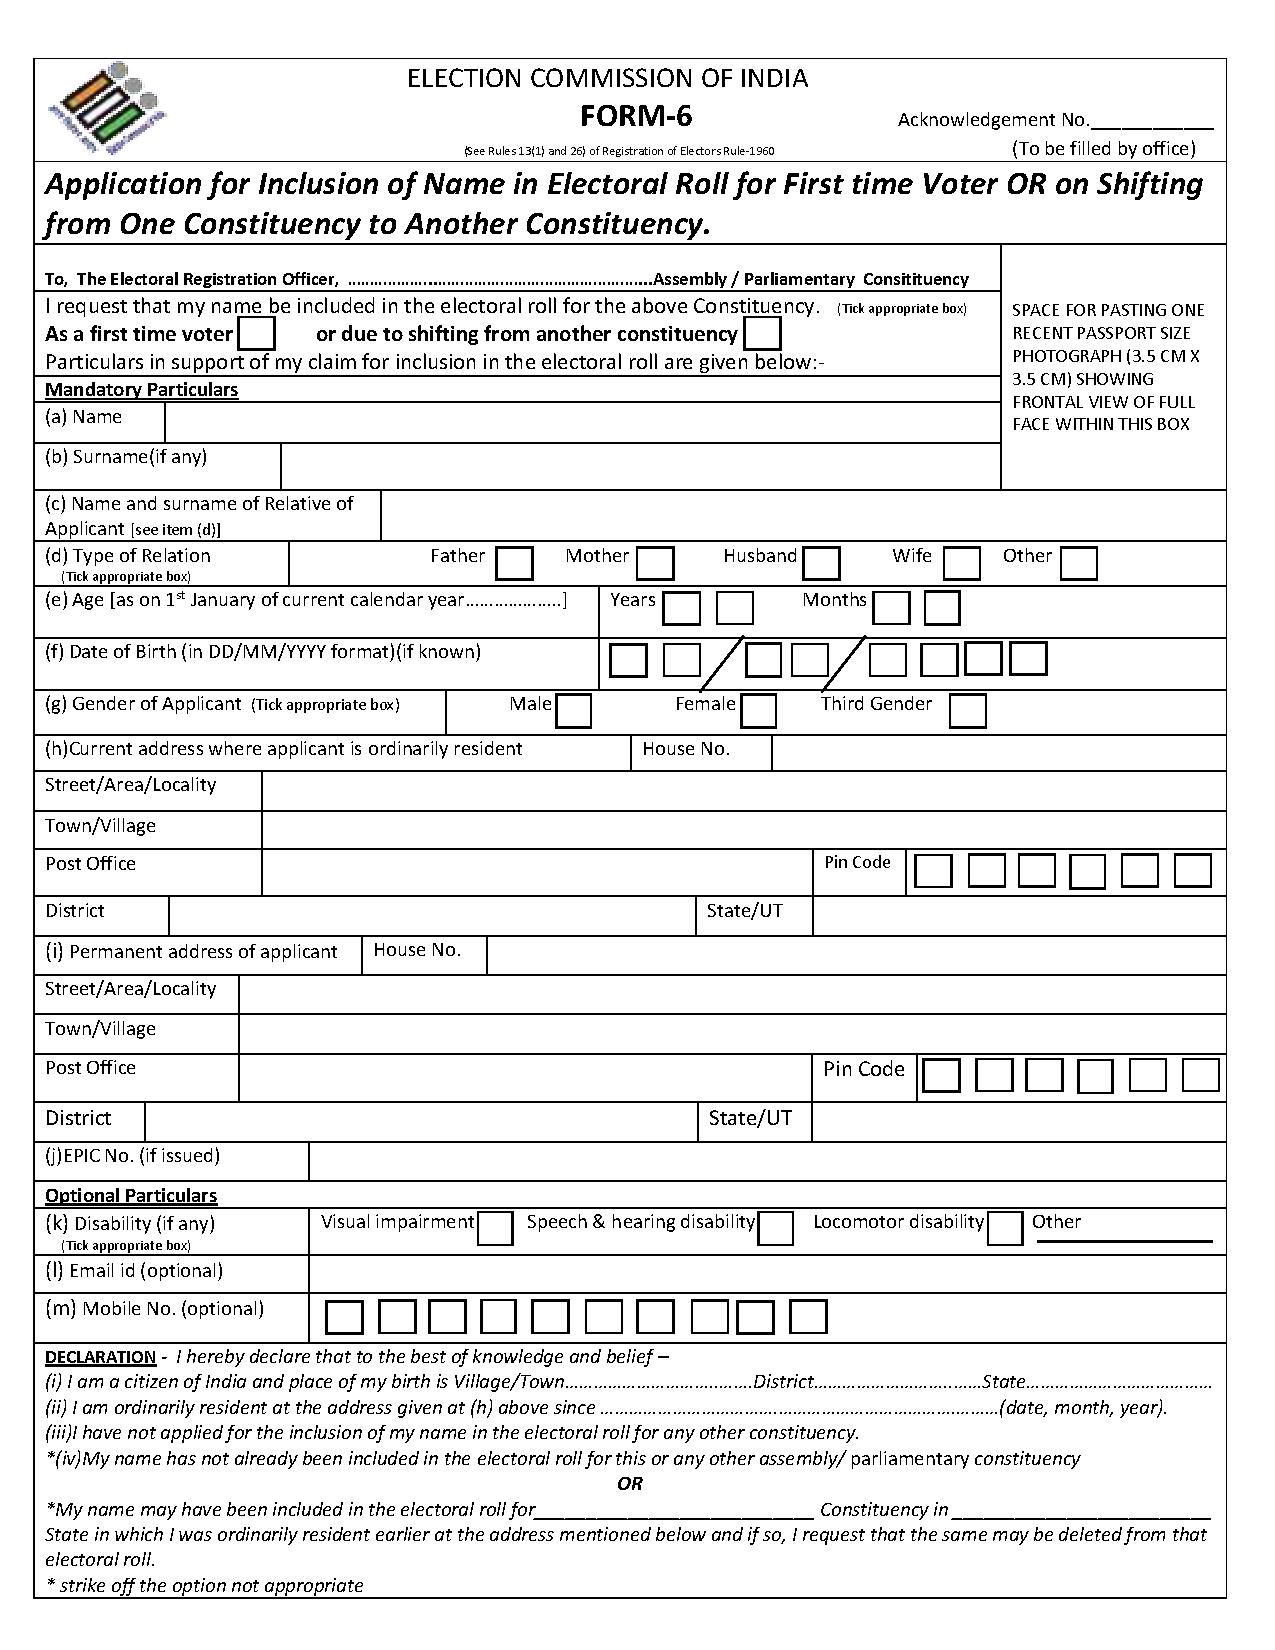
\includegraphics[width=0.5\linewidth]{pic-form-6-p1} 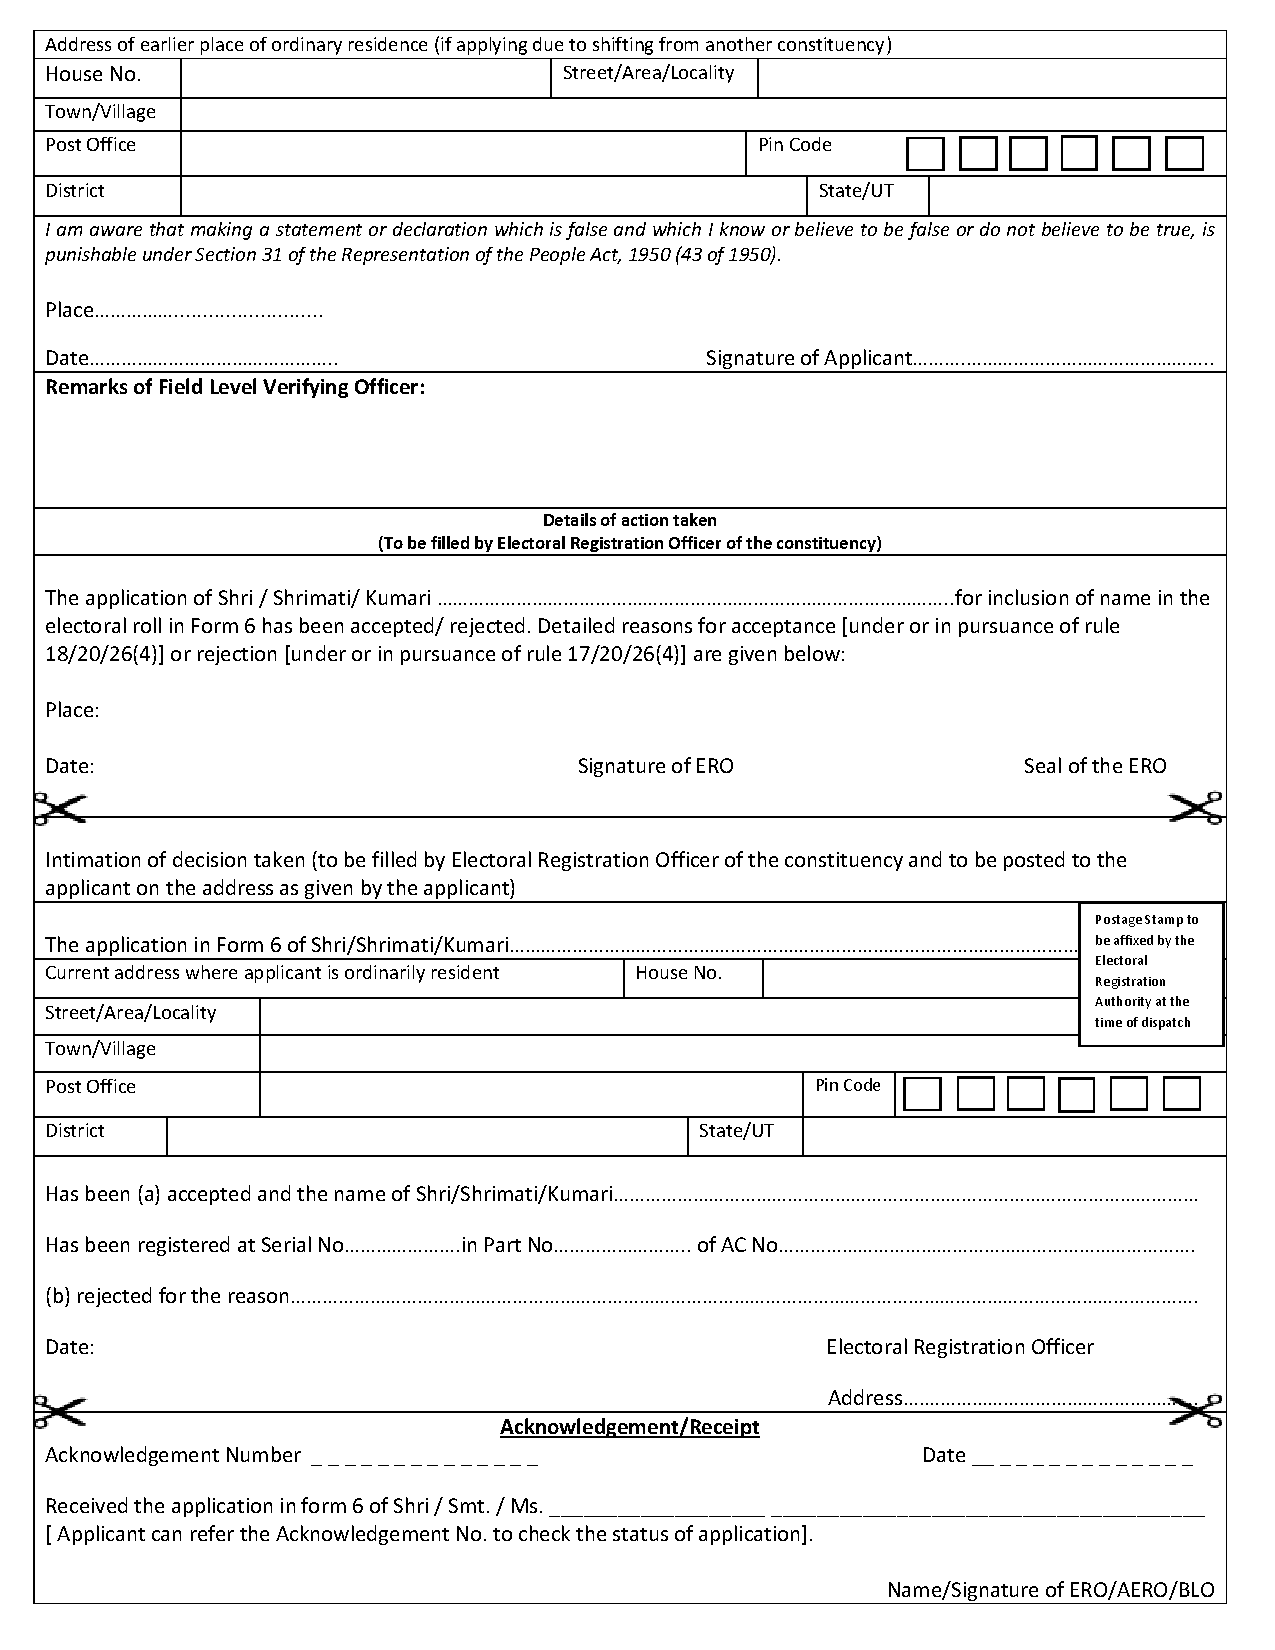
\includegraphics[width=0.5\linewidth]{pic-form-6-p2} \caption{Election Commission of India, Form 6.}\label{fig:unnamed-chunk-27}
\end{figure}

\begin{figure}
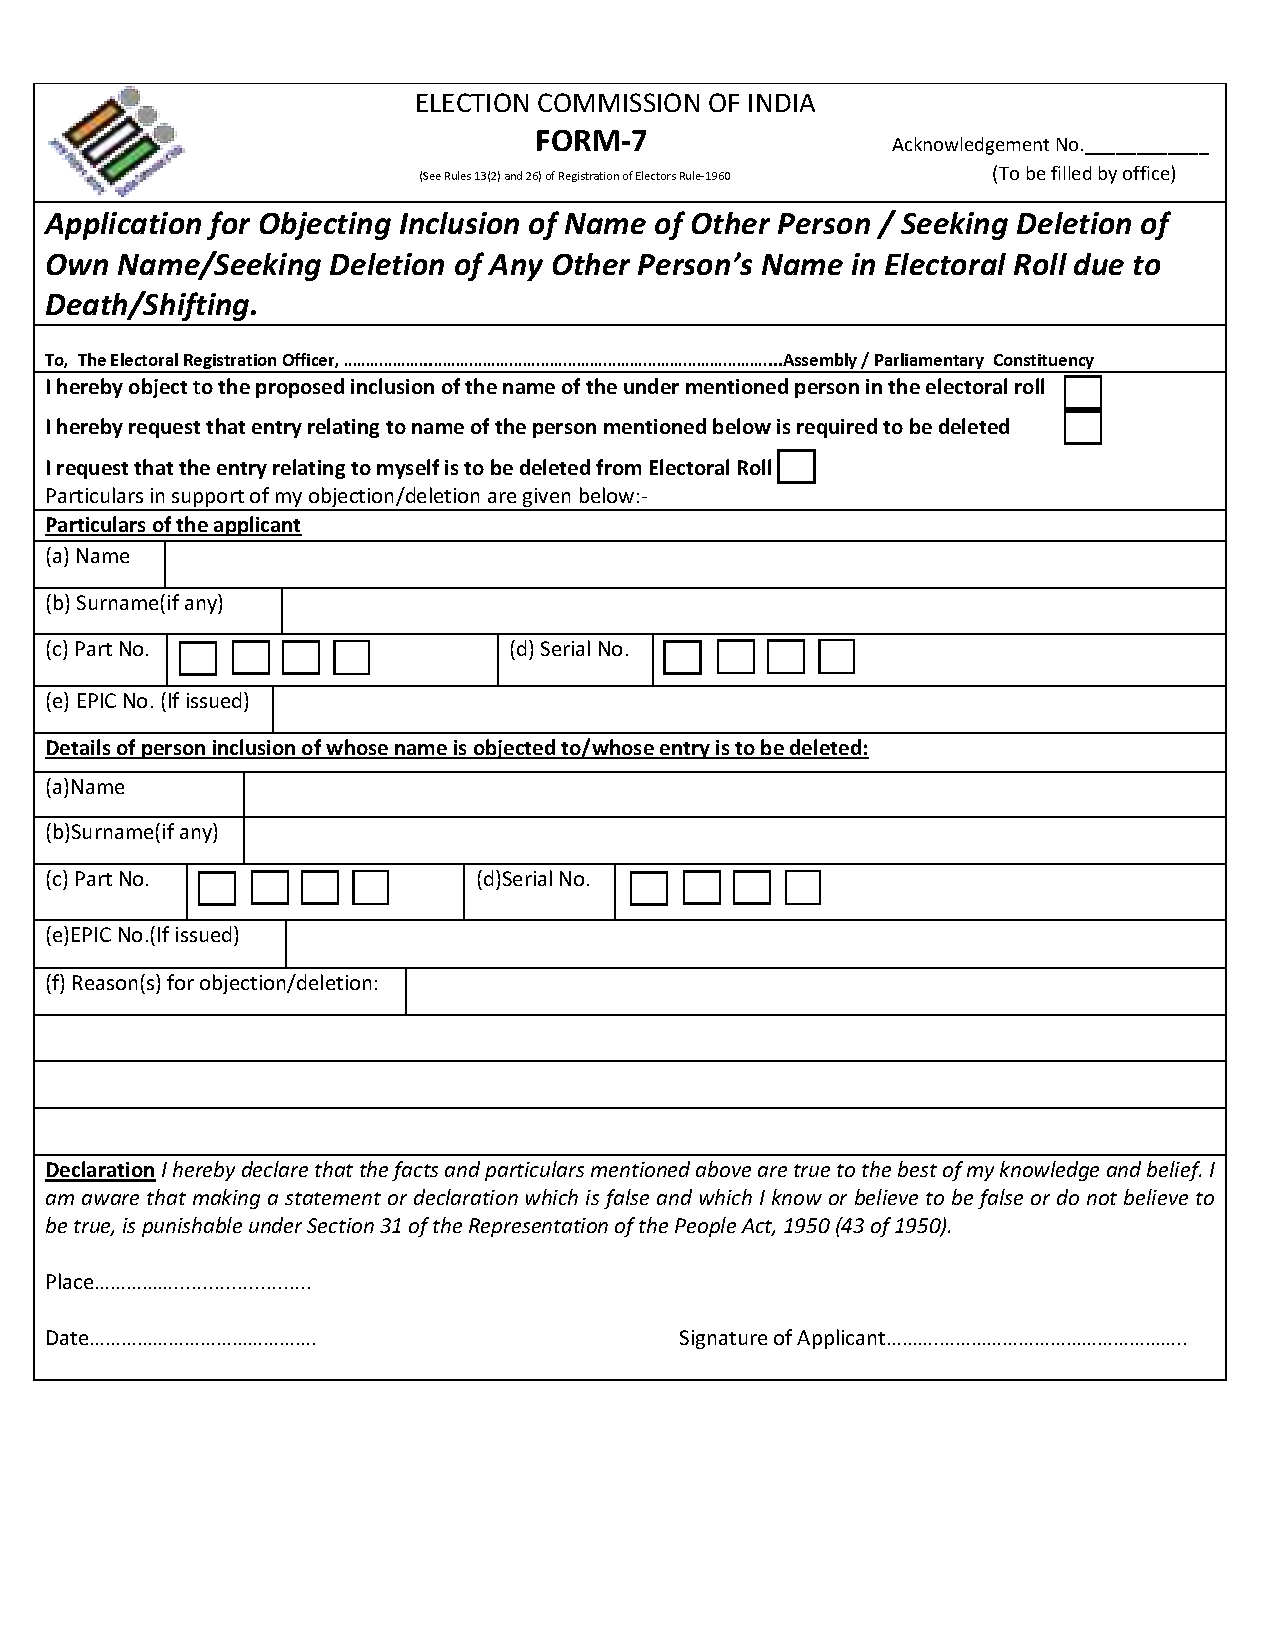
\includegraphics[width=0.5\linewidth]{pic-form-7-p1} 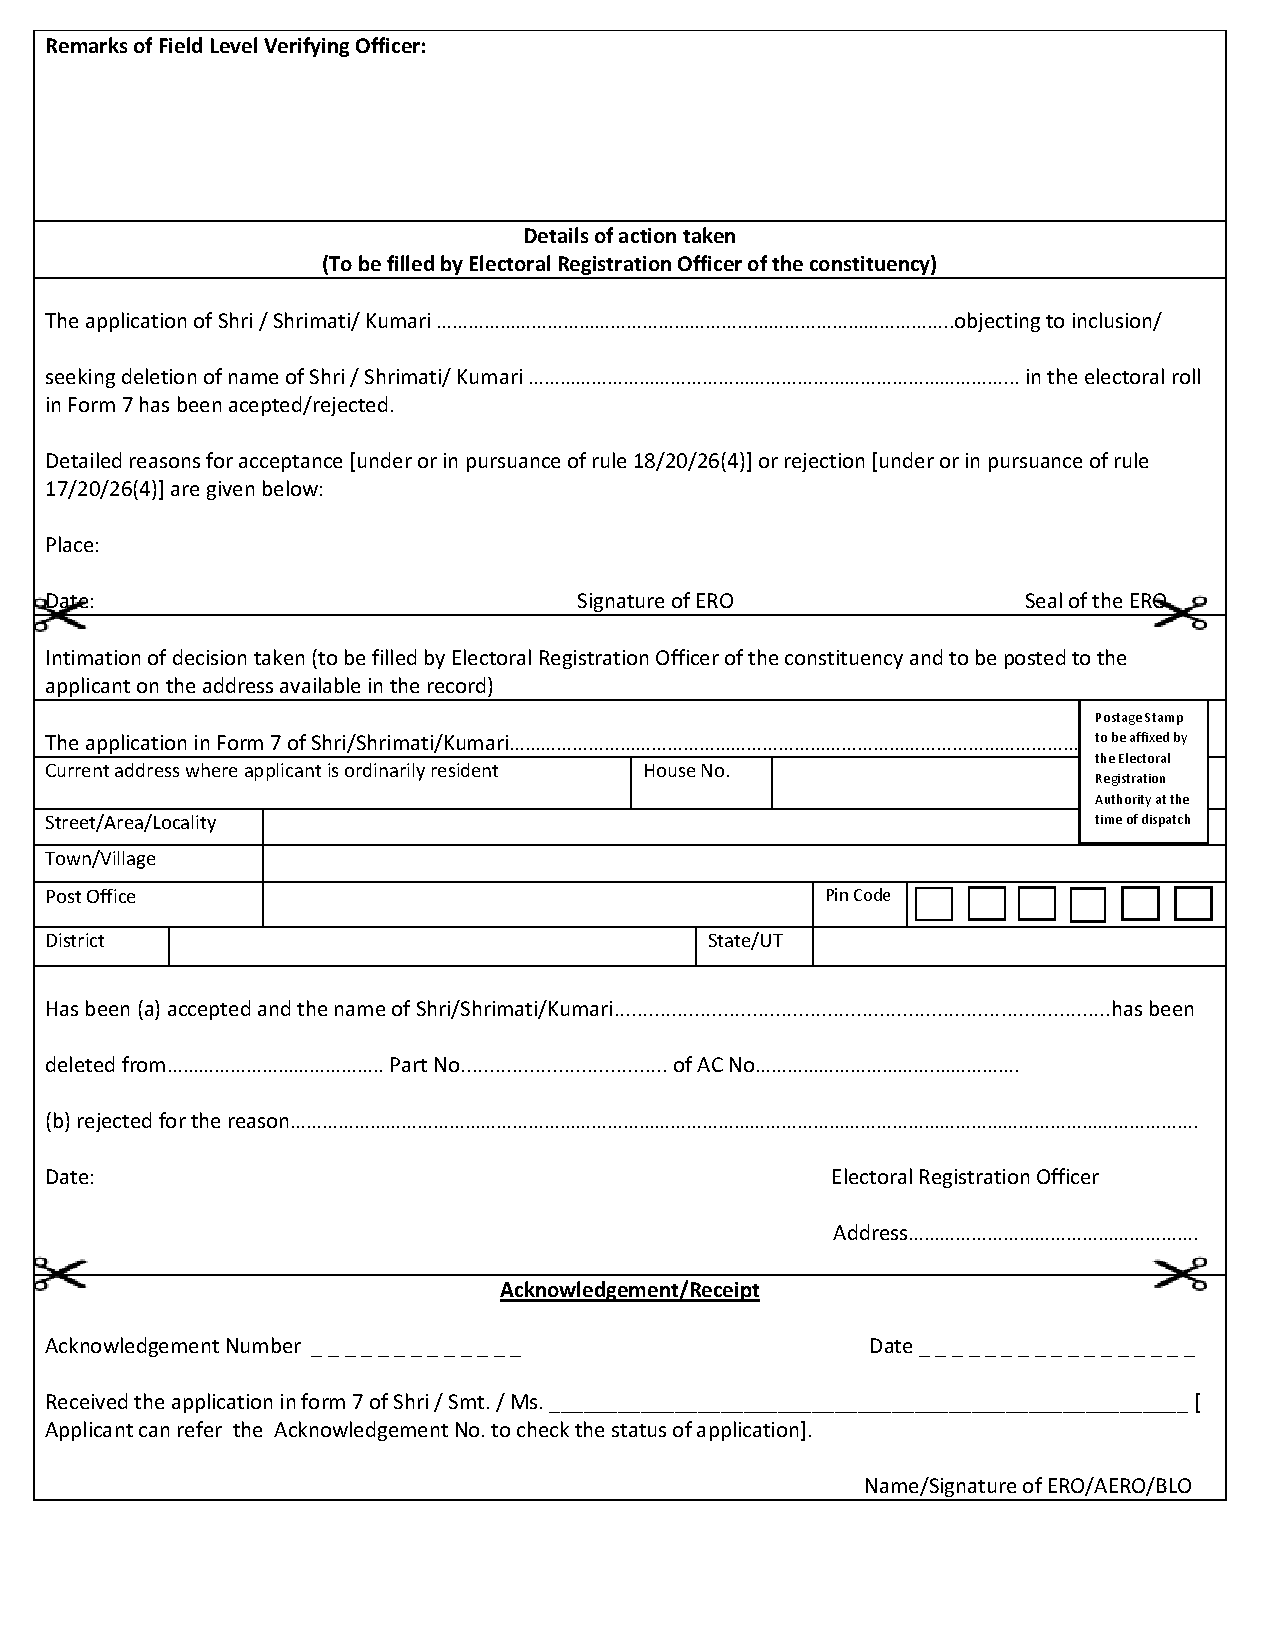
\includegraphics[width=0.5\linewidth]{pic-form-7-p2} \caption{Election Commission of India, Form 7.}\label{fig:unnamed-chunk-28}
\end{figure}

\subsection{Implementation of T1 in the field}

\begin{figure}
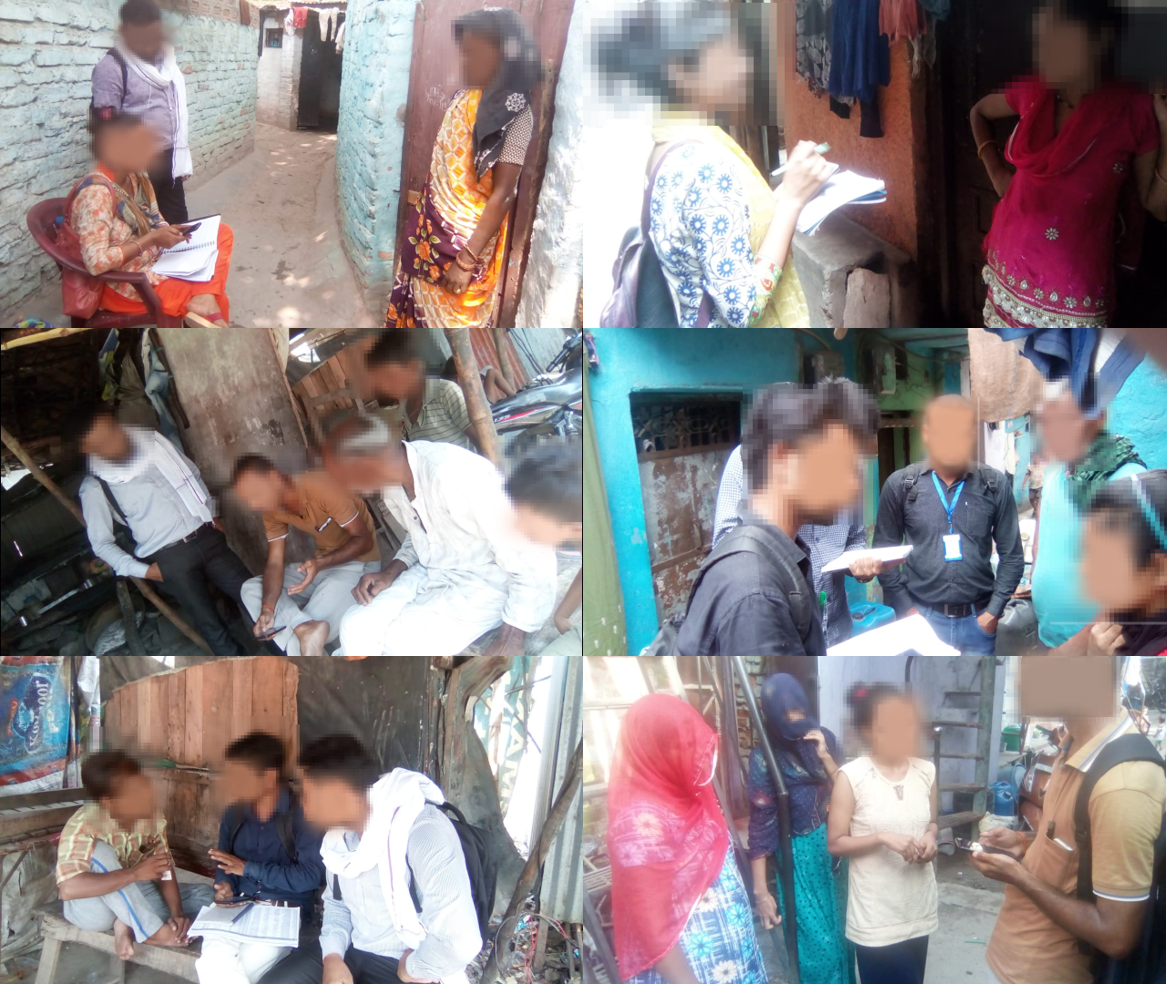
\includegraphics[width=1\linewidth]{pic-fieldteam} \caption{Photographs of field workers assisting T1-assigned migrants in gathering documents and filling in the forms needed to register to vote locally.}\label{fig:unnamed-chunk-29}
\end{figure}

\begin{figure}
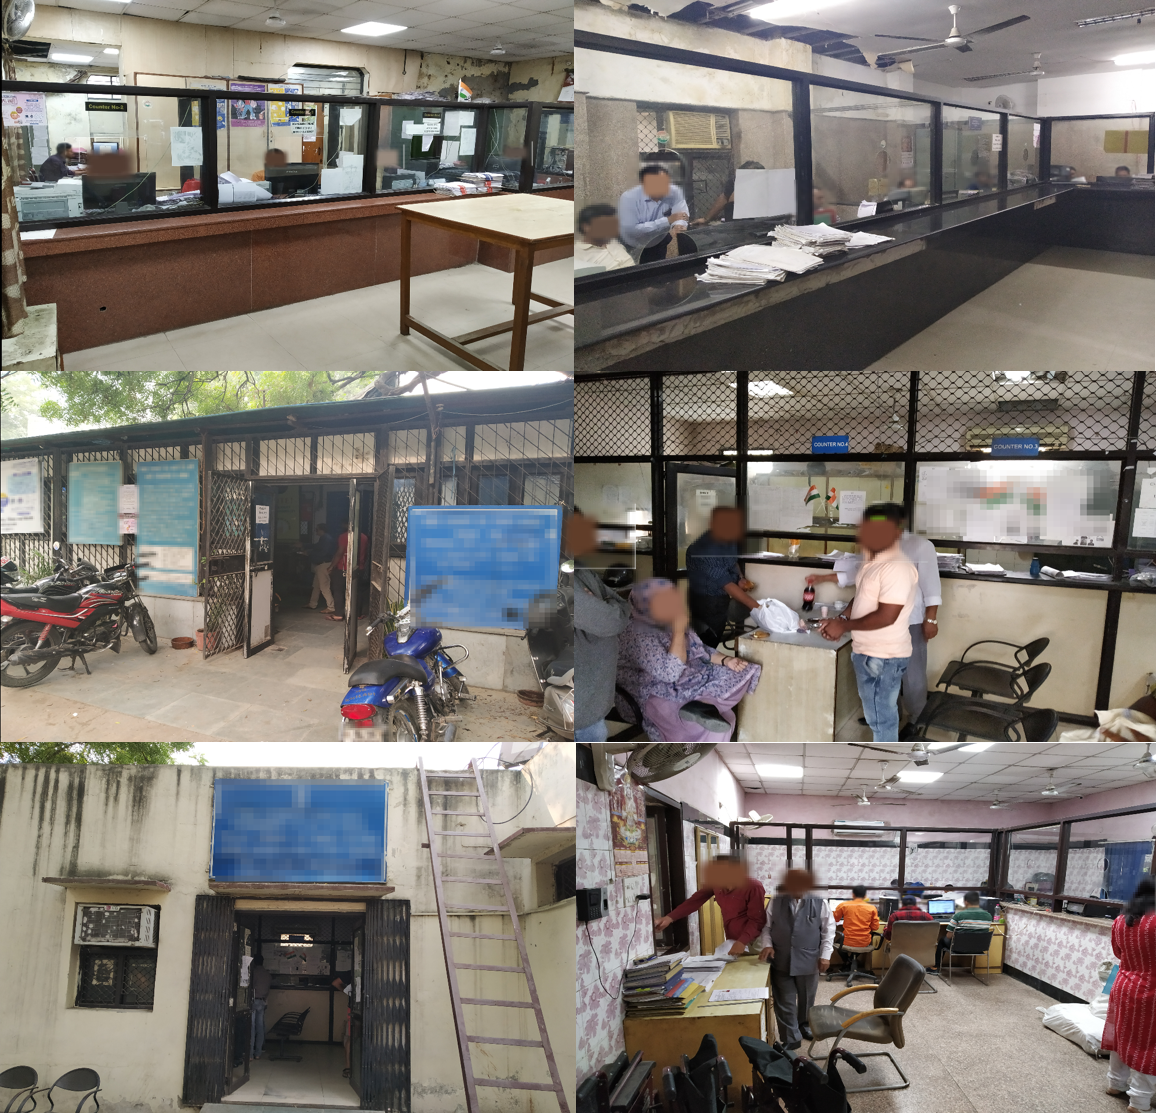
\includegraphics[width=1\linewidth]{pic-offices} \caption{Pictures of the local election offices where applications to register to vote are evaluated and processed.}\label{fig:unnamed-chunk-30}
\end{figure}

\begin{figure}
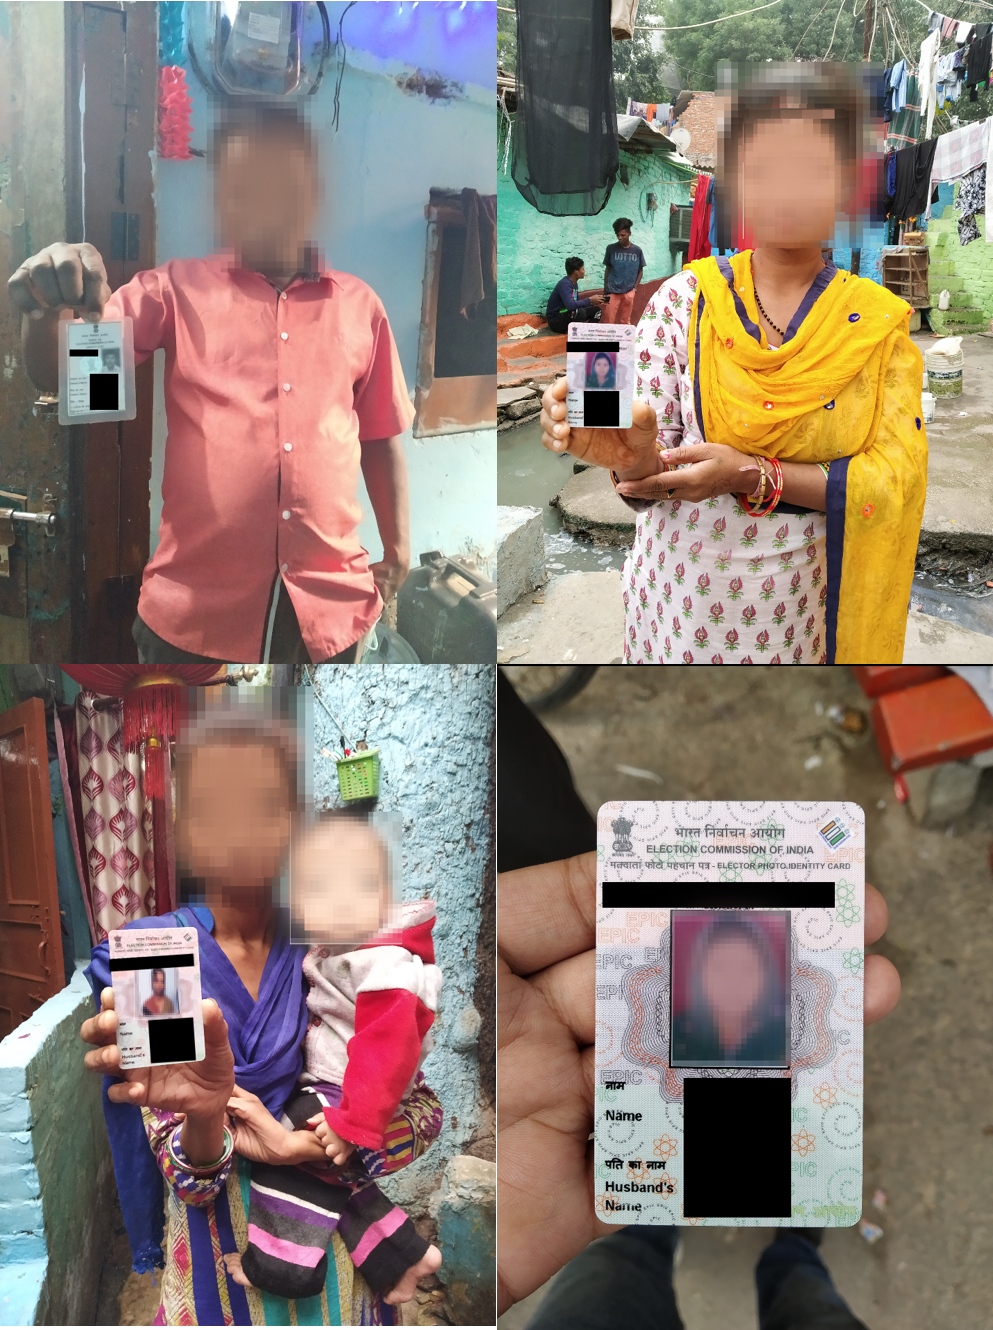
\includegraphics[width=1\linewidth]{pic-voter-id} \caption{Successful applicants hold up their newly minted voter ID cards, enabling them to vote locally.}\label{fig:unnamed-chunk-31}
\end{figure}

\section{Political parties and migrant outreach}

Are political parties in our study cities less likely to engage with
migrants than with long-term city residents in typical elections? To
address this question, we obtained proprietary data from the Centre for
Developing Societies (CSDS), which conducted a representative poll of
Delhi citizens following the 2015 state assembly elections there. The
survey was unique in that it elicited detailed information about
interactions with party workers in the lead-up to the election, broken
down by political party. Specifically, the survey instrument asked:
``Did any candidate, party worker or canvasser come to your house during
the campaign to ask for your vote?'' If the respondent answered in the
affirmative, they were then asked, ``Candidates or workers of which
party came to you?'' (they were able to list up to two parties).
Respondents were additionally asked, ``For how many years have you been
living in Delhi?'' with four response options provided. We employ the
definition of recent migrants employed in Banerjee and Kumar (2017):
those who have been living in Delhi for less than ten years.

We run a simple analysis to estimate whether migrants were less likely
to be visited by party canvassers compared to longer-term residents (see
Table \ref{tab:party_canvass}). We find strong evidence that this is
what occurred. Migrants were 14 percentage points less likely to be
visited by a party worker of any stripe---a difference that is
qualitatively large and statistically significant. We also examine
differences in visits by the various parties. The effects are negatively
signed for visits by canvassers from all the major parties, but are
largest and statistically significant for those campaigning on behalf of
the BJP.

These results lend credence to the claim that political parties are less
likely to engage in outreach to migrant citizens, plausibly on account
of their greater uncertainty about migrants' political preferences.

\begin{table}[!htbp] \centering 
  \caption{Canvassing visits to recent migrants versus long-term city residents in Delhi during the 2015 Delhi state assembly elections. Survey data were obtained from the Centre for the Study of Developing Societies and are described at: bit.ly/3nCrACa. Bivariate OLS analysis with robust standard errors in parentheses.} 
  \label{tab:party_canvass} 
\small 
\begin{tabular}{@{\extracolsep{5pt}}lcccc} 
\\[-1.8ex]\hline 
\hline \\[-1.8ex] 
 & \multicolumn{4}{c}{\textit{Dependent variable:}} \\ 
\cline{2-5} 
\\[-1.8ex] & \shortstack{Party \\ Canvasser \\ Visited} & \shortstack{AAP \\ Canvasser} & \shortstack{BJP \\ Canvasser} & \shortstack{INC \\ Canvasser} \\ 
\\[-1.8ex] & (1) & (2) & (3) & (4)\\ 
\hline \\[-1.8ex] 
 Migrant & $-$0.136$^{***}$ & $-$0.066 & $-$0.089$^{**}$ & $-$0.038 \\ 
  & (0.047) & (0.044) & (0.044) & (0.033) \\ 
  Constant & 0.632$^{***}$ & 0.412$^{***}$ & 0.443$^{***}$ & 0.187$^{***}$ \\ 
  & (0.011) & (0.011) & (0.011) & (0.009) \\ 
 \hline \\[-1.8ex] 
Observations & 1,994 & 2,060 & 2,060 & 2,060 \\ 
Adjusted R$^{2}$ & 0.004 & 0.001 & 0.001 & 0.0001 \\ 
\hline 
\hline \\[-1.8ex] 
\multicolumn{5}{r}{$^{*}$p$<$0.1; $^{**}$p$<$0.05; $^{***}$p$<$0.01} \\ 
\end{tabular} 
\end{table}

\section{T2 further information}

\begin{figure}

{\centering 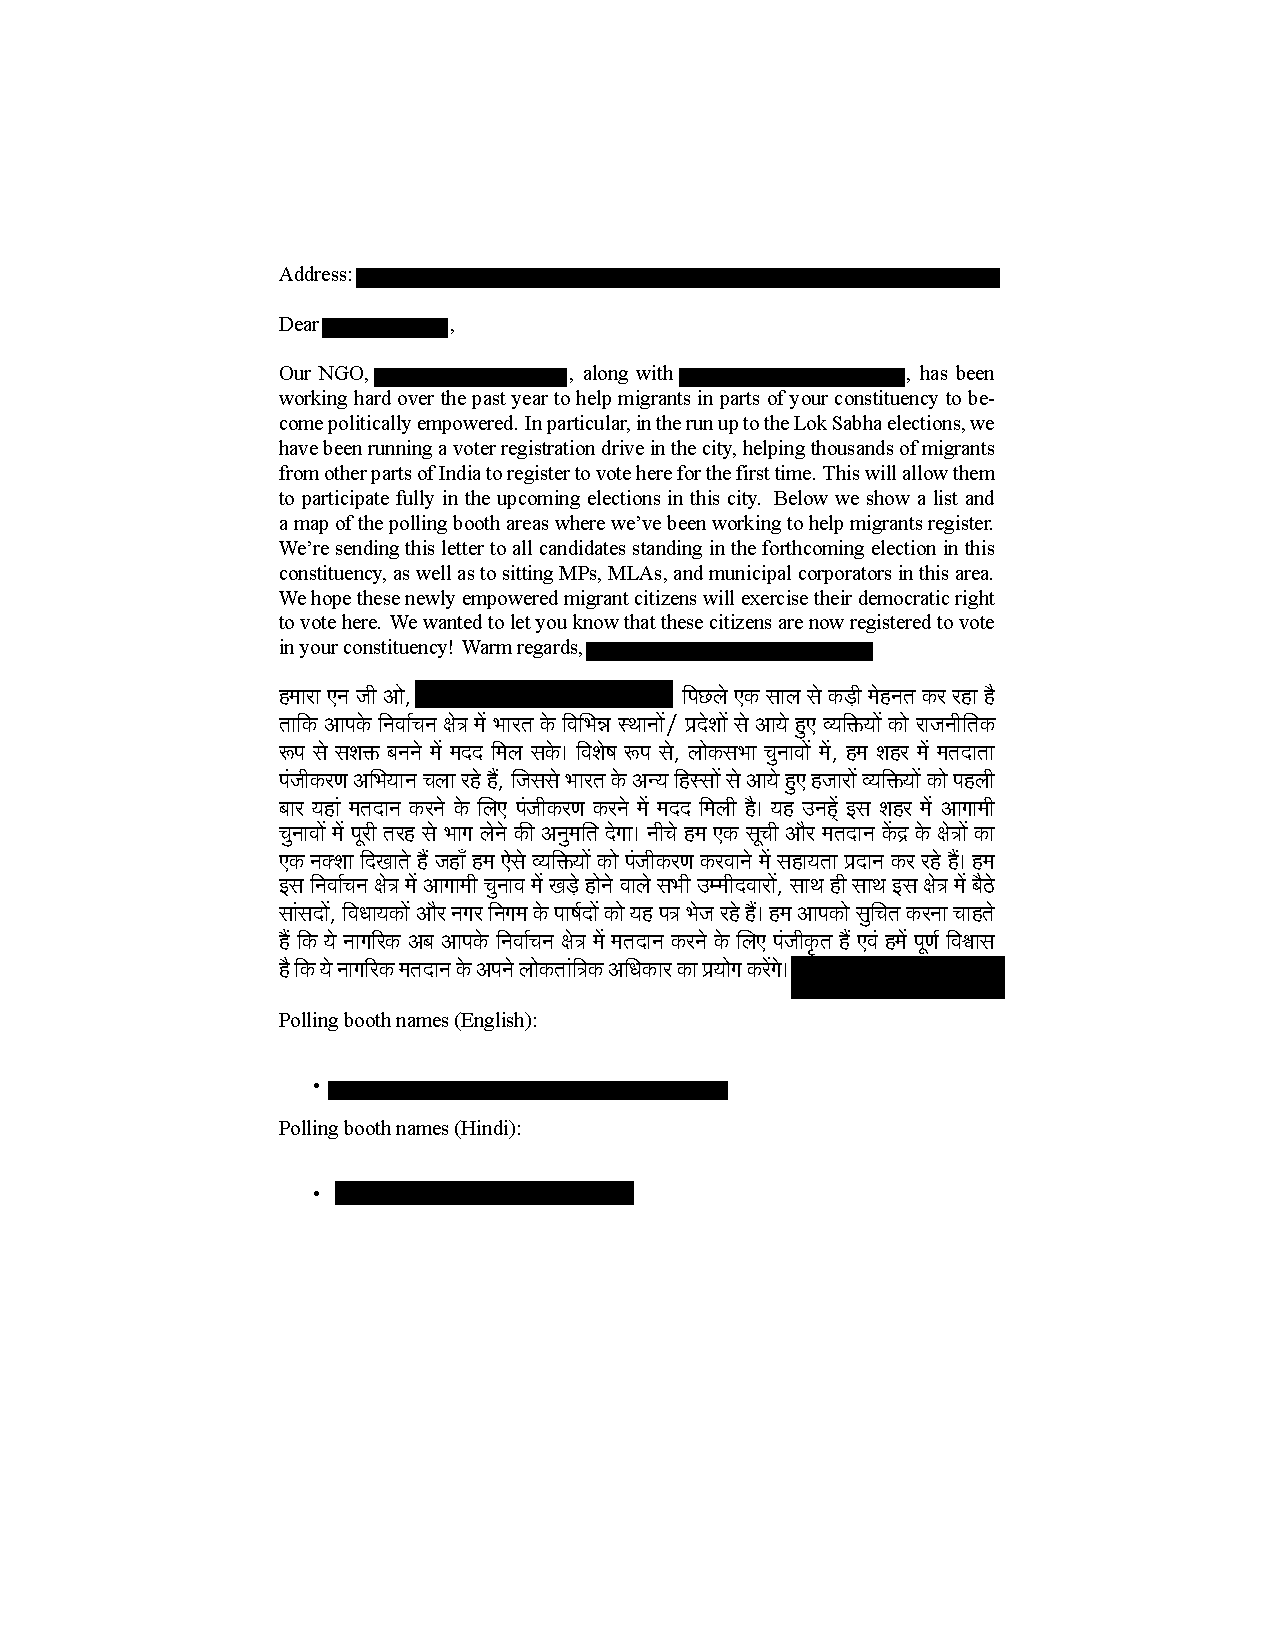
\includegraphics[width=0.7\linewidth]{pic-t2-letter} 

}

\caption{Example of typed letter mailed to local politicians in the lead up to the 2019 elections in T2 treated clusters. For confidentiality, identifying content is redacted and the referenced map is omitted.}\label{fig:unnamed-chunk-33}
\end{figure}

\begin{figure}

{\centering 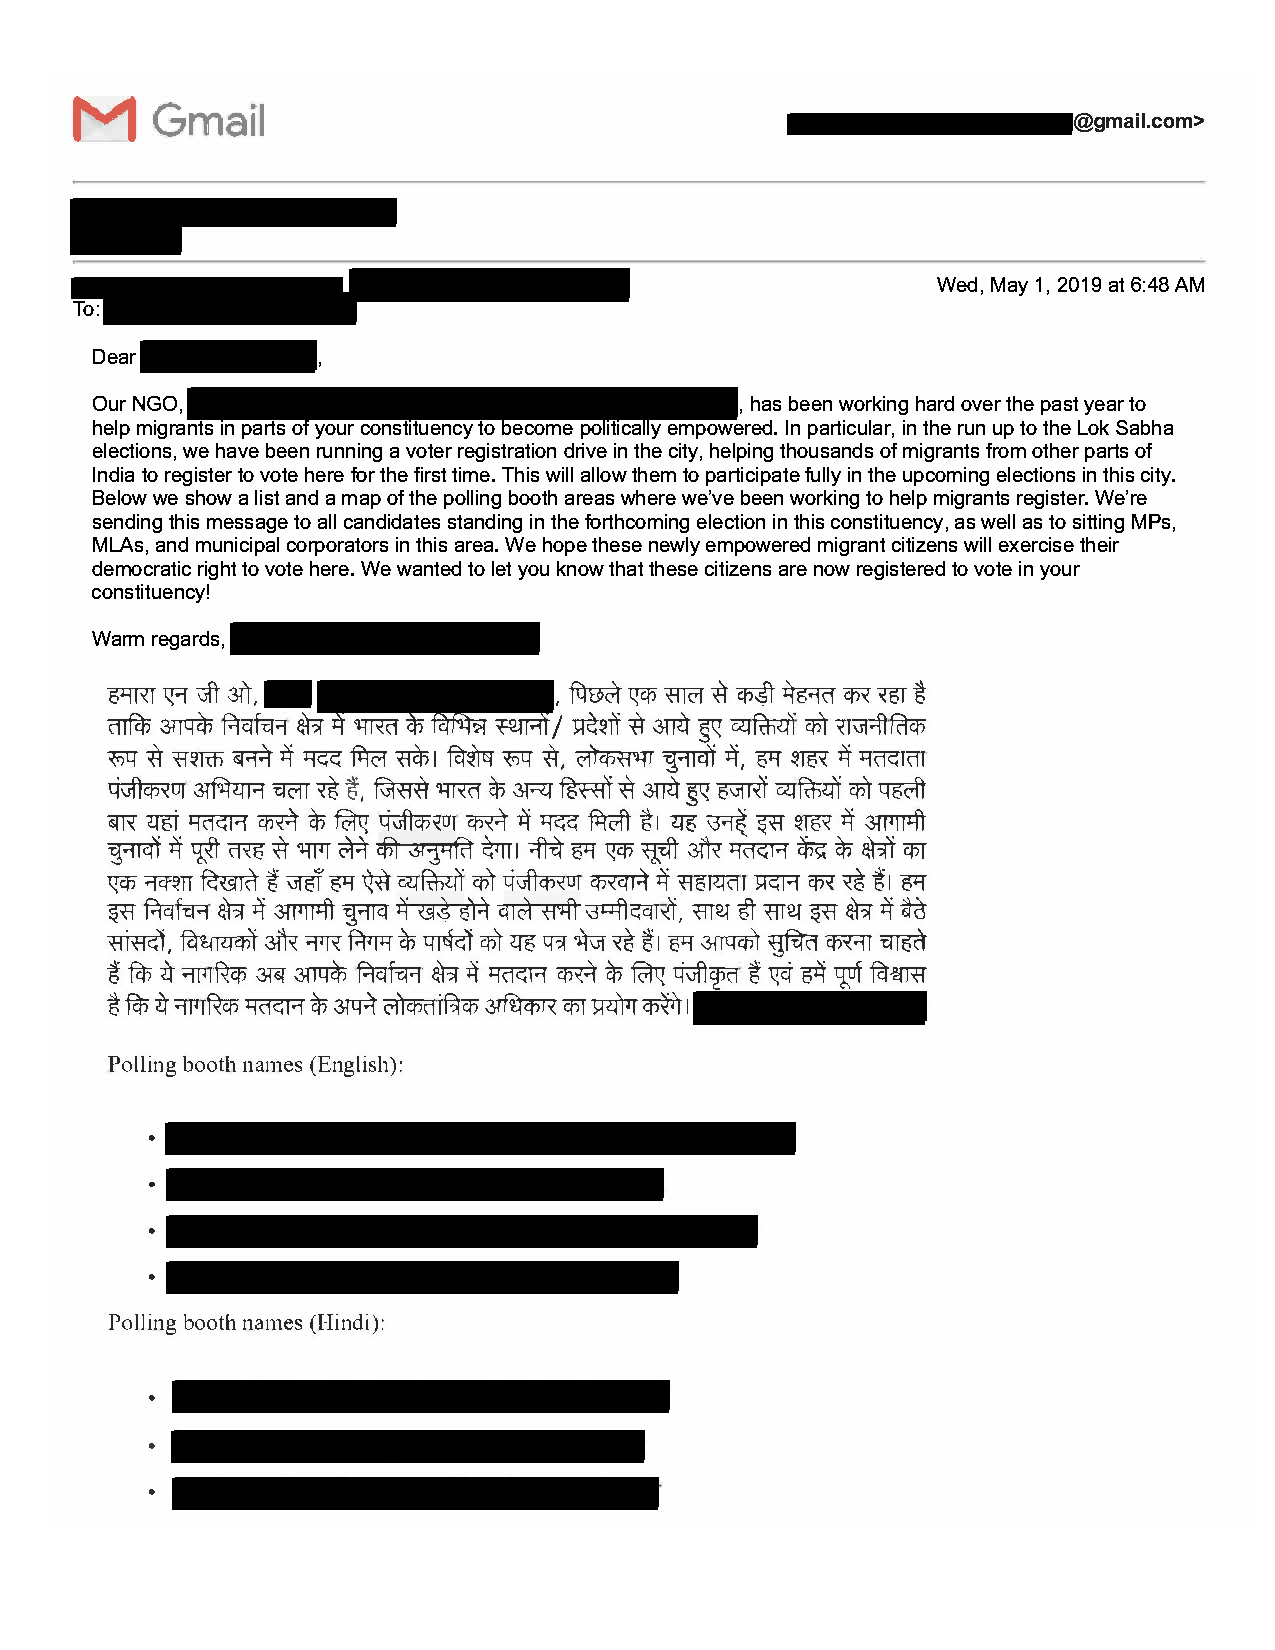
\includegraphics[width=0.7\linewidth]{pic-t2-email} 

}

\caption{Example of email sent to local politicians in the lead up to the 2019 elections in T2 treated clusters. For confidentiality, identifying content is redacted and the referenced map is omitted.}\label{fig:unnamed-chunk-34}
\end{figure}

\begin{figure}

{\centering 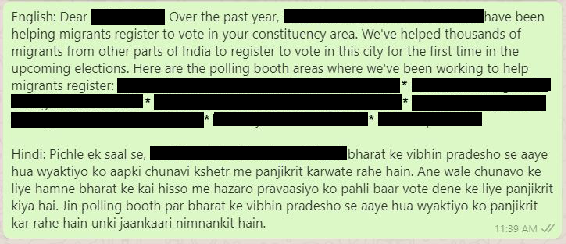
\includegraphics[width=0.7\linewidth]{pic-t2-whatsapp} 

}

\caption{Example of WhatsApp message sent to local politicians in the lead up to the 2019 elections in T2 treated clusters. For confidentiality, identifying content is redacted.}\label{fig:unnamed-chunk-35}
\end{figure}

\begin{figure}

{\centering 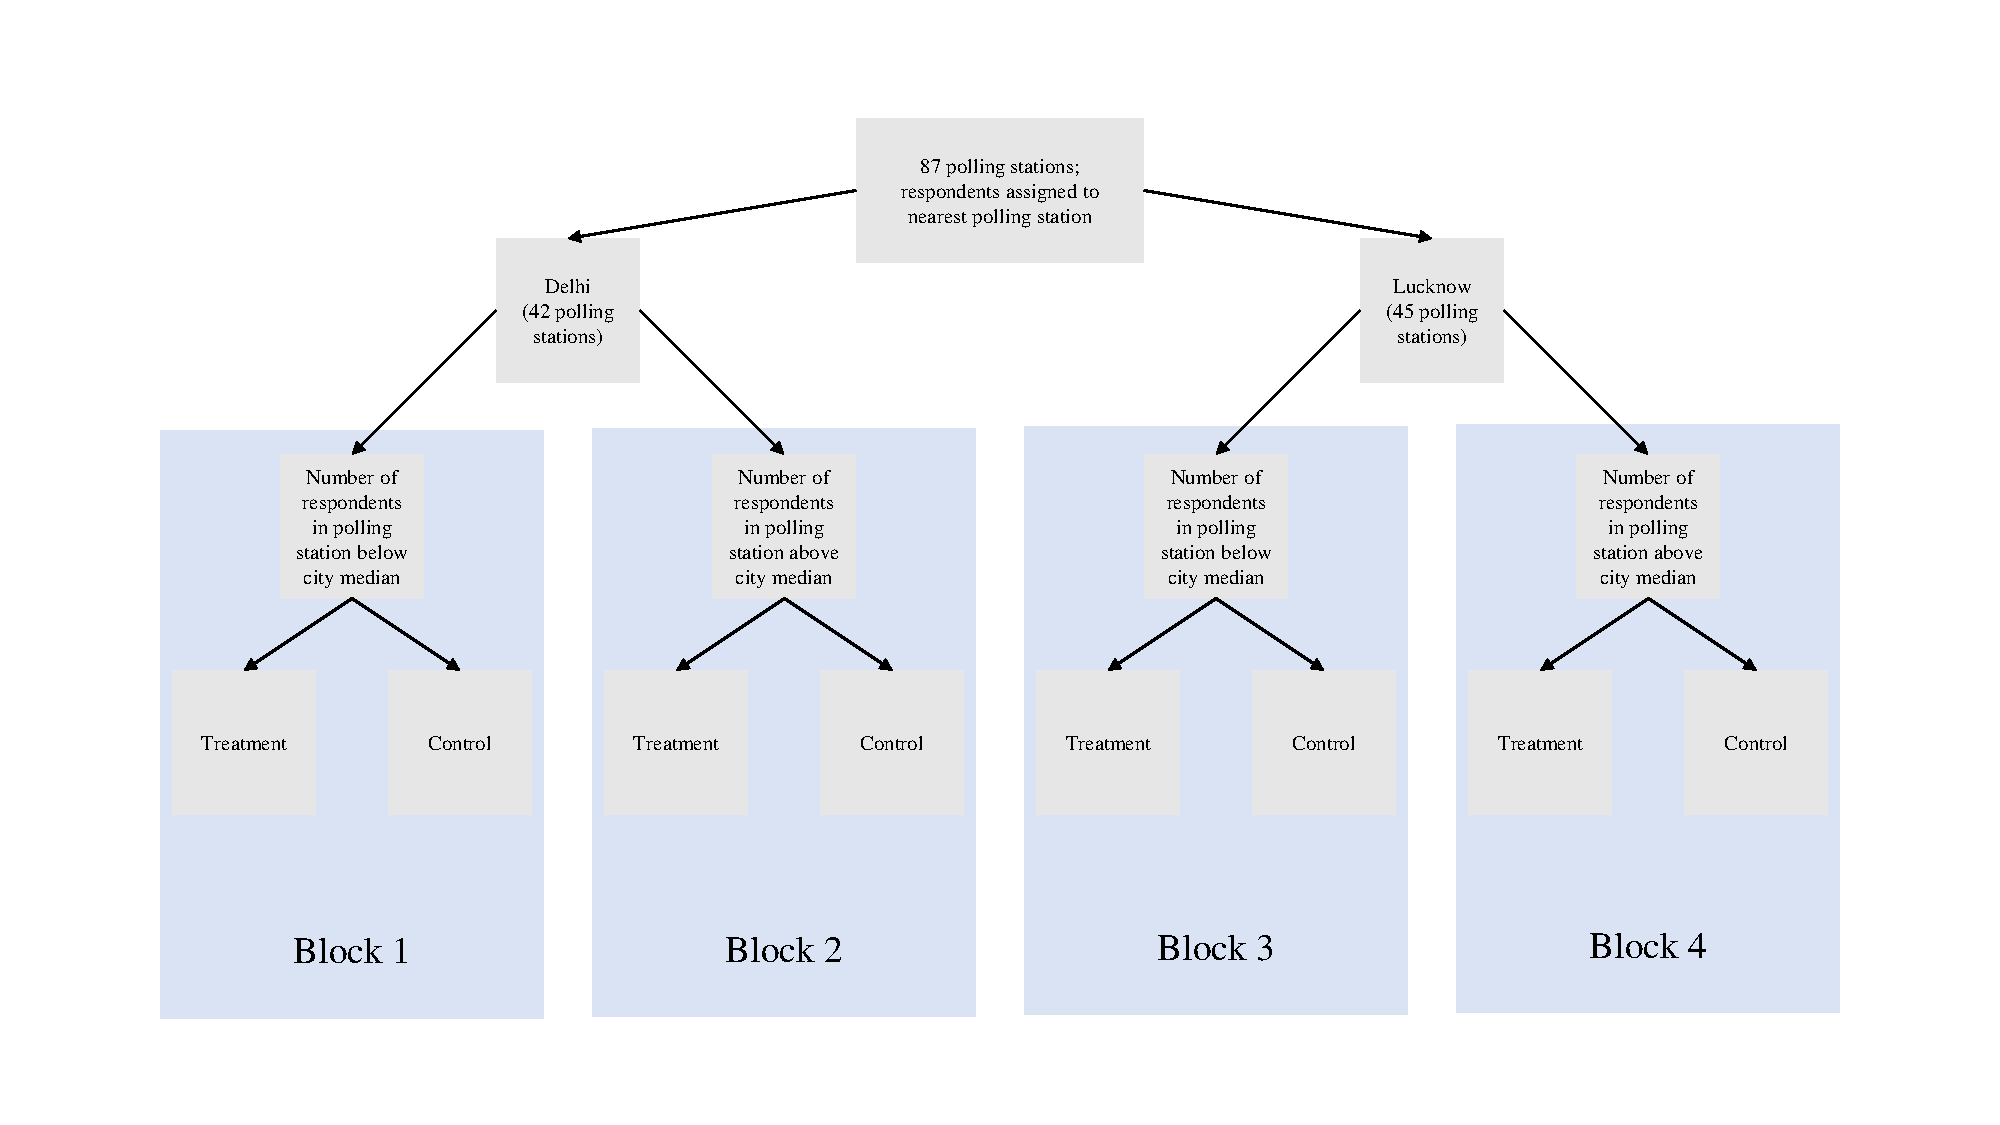
\includegraphics[width=1\linewidth]{pic-t2-block-design} 

}

\caption{Flow diagram of T2 randomization blocks. Clusters (polling stations) are assigned to T2 treatment or control within four blocks.}\label{fig:unnamed-chunk-36}
\end{figure}

\clearpage

\section{Study timeline}

\begin{figure}
\centering
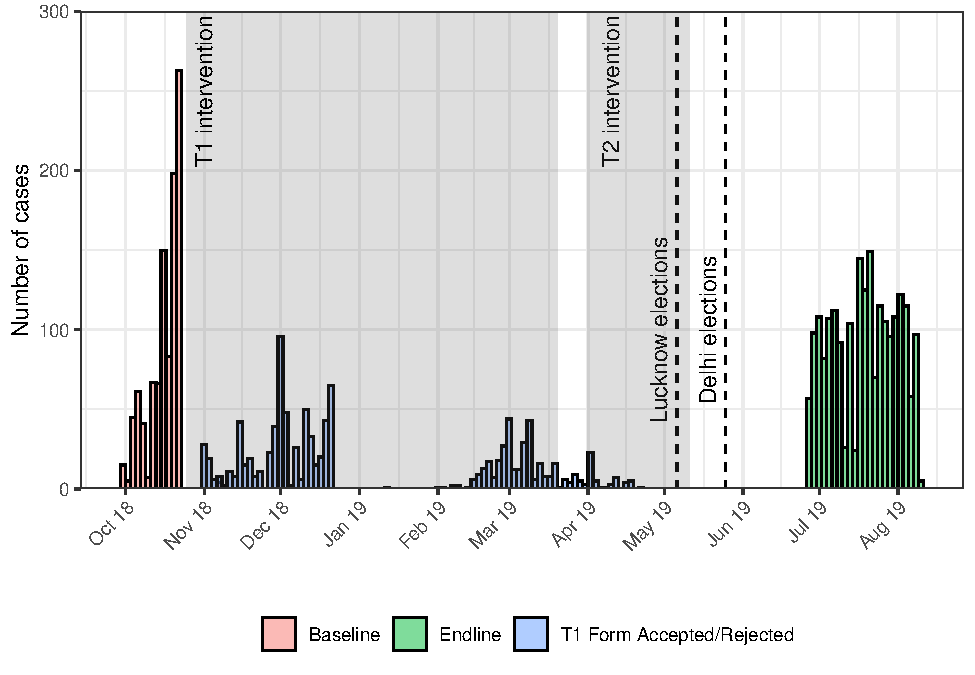
\includegraphics{supplementary-information_files/figure-latex/unnamed-chunk-37-1.pdf}
\caption{Study phasing. Red and green bars show the timing of the
surveys. Blue bars show the timing of final voter registration
application decisions, as reported in online administrative data.}
\end{figure}

\clearpage

\section{Indexing}

\begin{table}[!h]

\caption{\label{tab:unnamed-chunk-38}Index construction. Z-score indexes are constructed by coding component variables such that higher values are more beneficial. Component variables are then centered and standardized using the control group mean. The final index is then the average of the standardized components.}
\centering
\resizebox{\linewidth}{!}{
\fontsize{9}{11}\selectfont
\begin{tabular}[t]{ll>{\raggedright\arraybackslash}p{15em}l}
\toprule
Variable type & Indexed variable label & Component variable labels & Method of indexing\\
\midrule
\cellcolor{gray!6}{Outcome} & \cellcolor{gray!6}{Political interest} & \cellcolor{gray!6}{Interest in politics at the city level (ordinal); Interest in politics at the national level (ordinal)} & \cellcolor{gray!6}{Z-score index}\\
Outcome & Political trust & Trust in national government (ordinal); Trust in state government (ordinal); Trust in municipal corporation (ordinal); Trust in parties (ordinal) & Z-score index\\
\cellcolor{gray!6}{Outcome} & \cellcolor{gray!6}{Contacting city officials} & \cellcolor{gray!6}{Contacting officials (categorical)} & \cellcolor{gray!6}{Sum}\\
Outcome & Non-electoral participation & Non-electoral participation (categorical) & Sum\\
\cellcolor{gray!6}{Outcome} & \cellcolor{gray!6}{Campaign exposure} & \cellcolor{gray!6}{Basti visits by politicians (integer); Home visit by politician or party worker (integer); Number of gifts (integer); Migrant-focused campaigning (binary); Perceived campaign intensity (ordinal)} & \cellcolor{gray!6}{Z-score index}\\
Lagged DV & Political trust & Trust in national government (ordinal); Trust in state government (ordinal); Trust in municipal corporation (ordinal) & Z-score index\\
\cellcolor{gray!6}{Lagged DV} & \cellcolor{gray!6}{Politician visits} & \cellcolor{gray!6}{Politician visits to basti, by municipal corporator, MLA, and MP} & \cellcolor{gray!6}{Sum}\\
\bottomrule
\end{tabular}}
\end{table}

\clearpage

\section{Outliers in `income` covariate}

When cleaning the data we observed several extreme outliers in the
\texttt{income} covariate. To minimize the influence of these extreme
values, we winsorize the variable, setting all values above the value of
the 99th percentile to the value of the 99th percentile itself. The
transformed variable is used in all statistical analyses.

\begin{figure}
\centering
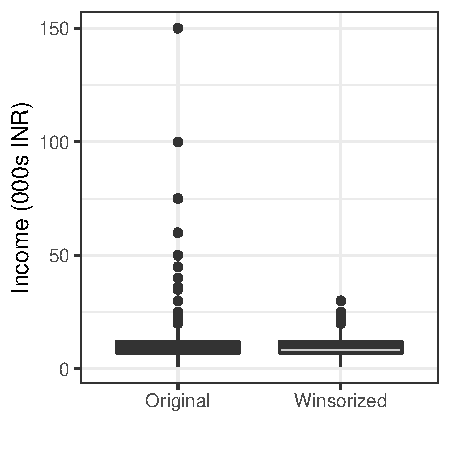
\includegraphics{supplementary-information_files/figure-latex/unnamed-chunk-39-1.pdf}
\caption{Box plots show the distribution of the raw income covariate
before and after winsorizing.}
\end{figure}

\clearpage

\section{Internal validity}

\subsection{Balance}

\begin{table}[!htbp] \centering 
  \caption{T1 balance test for subjects included in T1 analyses. OLS regression. All covariates are measured at baseline. Robust standard errors in parentheses.} 
  \label{} 
\small 
\begin{tabular}{@{\extracolsep{5pt}}lc} 
\\[-1.8ex]\hline 
\hline \\[-1.8ex] 
 & \multicolumn{1}{c}{\textit{Dependent variable:}} \\ 
\cline{2-2} 
\\[-1.8ex] & T1 treatment indicator \\ 
\hline \\[-1.8ex] 
 Female & 0.016 (0.025) \\ 
  Age & $-$0.001 (0.001) \\ 
  Muslim & 0.017 (0.028) \\ 
  SC/ST & 0.001 (0.025) \\ 
  Primary education & $-$0.010 (0.026) \\ 
  Income (INR 000s) & 0.002 (0.002) \\ 
  Married & $-$0.038 (0.029) \\ 
  Length of residence in city & 0.002$^{*}$ (0.001) \\ 
  Owns home in city & 0.058$^{**}$ (0.025) \\ 
  Hadn't voted previously & 0.044 (0.041) \\ 
  How likely to vote in city if registered & $-$0.010 (0.060) \\ 
  Political interest & $-$0.040 (0.041) \\ 
  Sense of political efficacy & $-$0.031 (0.031) \\ 
  Political trust index & 0.004 (0.015) \\ 
  Shared meal with non-coethnic & $-$0.012 (0.034) \\ 
  Has hometown voter ID & 0.013 (0.037) \\ 
  Returned to vote in hometown & 0.047 (0.042) \\ 
  More at home in hometown & 0.013 (0.034) \\ 
  Straight-line distance to home district & 0.00002 (0.00003) \\ 
  Still receives hometown schemes & $-$0.006 (0.024) \\ 
  Owns hometown property & 0.001 (0.026) \\ 
 \hline \\[-1.8ex] 
Pr(>F) of H0: joint orthogonality & 0.408 \\ 
Observations & 2,120 \\ 
Adjusted R$^{2}$ & 0.0004 \\ 
\hline 
\hline \\[-1.8ex] 
\multicolumn{2}{r}{$^{*}$p$<$0.1; $^{**}$p$<$0.05; $^{***}$p$<$0.01} \\ 
\end{tabular} 
\end{table}

\begin{table}[!htbp] \centering 
  \caption{T2 balance test for subjects included in T2 analyses. Weighted least squares regression. Clusters weighted equally. Model includes block fixed effects. All covariates are measured at baseline. Cluster-robust standard errors in parentheses.} 
  \label{} 
\small 
\begin{tabular}{@{\extracolsep{5pt}}lc} 
\\[-1.8ex]\hline 
\hline \\[-1.8ex] 
 & \multicolumn{1}{c}{\textit{Dependent variable:}} \\ 
\cline{2-2} 
\\[-1.8ex] & T2 treatment indicator \\ 
\hline \\[-1.8ex] 
 Politician visits & $-$0.008 (0.035) \\ 
  Female & 0.018 (0.039) \\ 
  Age & 0.001 (0.002) \\ 
  Muslim & 0.121 (0.078) \\ 
  SC/ST & 0.003 (0.056) \\ 
  Primary education & 0.001 (0.042) \\ 
  Income (INR 000s) & 0.011$^{**}$ (0.004) \\ 
  Married & 0.007 (0.049) \\ 
  Length of residence in city & 0.002 (0.002) \\ 
  Owns home in city & 0.004 (0.058) \\ 
 \hline \\[-1.8ex] 
Pr(>F) of H0: joint orthogonality & 0.406 \\ 
No. of clusters & 87 \\ 
Observations & 1,969 \\ 
Adjusted R$^{2}$ & 0.017 \\ 
\hline 
\hline \\[-1.8ex] 
\multicolumn{2}{r}{$^{*}$p$<$0.1; $^{**}$p$<$0.05; $^{***}$p$<$0.01} \\ 
\end{tabular} 
\end{table}

\clearpage

\subsection{Attrition rates by treatment condition}

\begin{table}[!htbp] \centering 
  \caption{Comparison of attrition rates across T1 treatment arms using OLS regression. The analysis includes all subjects randomized to T1 treatment or control. Robust standard errors in parentheses.} 
  \label{} 
\small 
\begin{tabular}{@{\extracolsep{5pt}}lc} 
\\[-1.8ex]\hline 
\hline \\[-1.8ex] 
 & \multicolumn{1}{c}{\textit{Dependent variable:}} \\ 
\cline{2-2} 
\\[-1.8ex] & Attrition Indicator \\ 
\hline \\[-1.8ex] 
 Assigned to T1 treatment & $-$0.007 (0.011) \\ 
 \hline \\[-1.8ex] 
Observations & 2,306 \\ 
Adjusted R$^{2}$ & $-$0.0003 \\ 
\hline 
\hline \\[-1.8ex] 
\multicolumn{2}{r}{$^{*}$p$<$0.1; $^{**}$p$<$0.05; $^{***}$p$<$0.01} \\ 
\end{tabular} 
\end{table}

\begin{table}[!htbp] \centering 
  \caption{Comparison of attrition rates across T2 treatment arms using weighted least squares regression. Clusters are weighted equally. Models include block fixed effects. The analysis includes all subjects randomized to T2 treatment or control. (Note that this number is smaller than that for the T1 attrition analysis as baseline geo-coordinates were unavailable for some subjects; hence they were not assigned to clusters or randomized.) Cluster-robust standard errors in parentheses.} 
  \label{} 
\small 
\begin{tabular}{@{\extracolsep{5pt}}lc} 
\\[-1.8ex]\hline 
\hline \\[-1.8ex] 
 & \multicolumn{1}{c}{\textit{Dependent variable:}} \\ 
\cline{2-2} 
\\[-1.8ex] & Attrition Indicator \\ 
\hline \\[-1.8ex] 
 Assigned to T2 treatment & $-$0.021 (0.021) \\ 
 \hline \\[-1.8ex] 
No. of clusters & 87 \\ 
Observations & 2,131 \\ 
Adjusted R$^{2}$ & 0.003 \\ 
\hline 
\hline \\[-1.8ex] 
\multicolumn{2}{r}{$^{*}$p$<$0.1; $^{**}$p$<$0.05; $^{***}$p$<$0.01} \\ 
\end{tabular} 
\end{table}

\clearpage

\hypertarget{administrative-data-on-t1-application-processing}{%
\section{Administrative data on T1 application
processing}\label{administrative-data-on-t1-application-processing}}

Because our field team helped applicants to submit the voter
registration forms online, we were able to track the progress of each
submitted case. Specifically, the Election Commission's online portal
provides the dates that applications were received and assigned to a
Booth Level Officer (BLO). It also gives the final date when the
application was either accepted or rejected. (No reasons are given for
rejection.) In Figure \ref{fig:t1_admin_hist}, we present histograms of
the time lapse for each of these various stages, as well as the median
times.

\begin{figure}
\centering
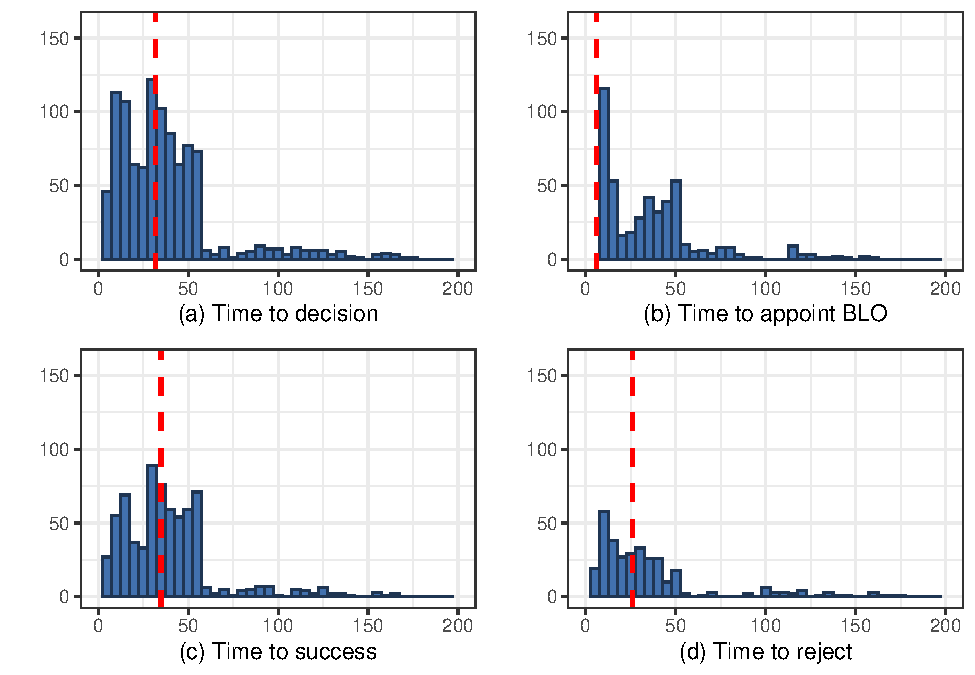
\includegraphics{supplementary-information_files/figure-latex/unnamed-chunk-44-1.pdf}
\caption{\label{fig:t1_admin_hist}This figure displays the distributions
of the time elapsed between the application submission dates and various
stages in the application processing, as reported in the online portal
of the Election Commission of India. The sample is for experimental
subjects assigned to T1 who submitted applications. Red vertical lines
display the median value. Note, cases that took longer than 200 days to
process are excluded.}
\end{figure}

\clearpage

\hypertarget{deviations-from-pre-analysis-plan}{%
\section{Deviations from pre-analysis
plan}\label{deviations-from-pre-analysis-plan}}

The study pre-analysis plan (PAP) was filed at the Evidence in
Governance and Politics registry before the researchers accessed the
endline data and prior to any data analysis being conducted. There were
two deviations from the pre-registered plan. First, the observational
data analyses described on pp.~6--7 of the PAP were not implemented as
there was insufficient variation in the outcome variable of interest
(whether eligible subjects wished to acquire a city-based voter ID card)
to make these tests feasible. This substantive finding is highlighted in
the paper. Second, in the endline data, there were 38 missing values for
the variable, \texttt{e\_campaign5\_exposure\_hardwork}. This is one of
five variables used in the construction of the index variable,
\texttt{e\_campaign\_exposure}. For the purposes of constructing this
index variable, the 38 missing values of
\texttt{e\_campaign5\_exposure\_hardwork} were imputed by sampling at
random from the non-missing values of that variable within the cluster
(polling station) to which the respondent belonged.

All remaining pre-registered experimental analyses in this paper are
implemented in conformity with the PAP.

\hypertarget{additional-ethical-considerations}{%
\section{Additional ethical
considerations}\label{additional-ethical-considerations}}

In this section, we detail features of our experimental design and
implementation that went above and beyond the minimal requirements
needed to secure Institutional Review Board (IRB) approval. We note that
exceeding IRB requirements has long been advocated by ethicists in the
discipline (e.g.~Tolleson-Rinehart 2008; Yanow and Schwartz-Shea 2008;
Teele 2014; Fujii 2012), and indeed, we heeded the general principles
outlined in existing guidelines when designing our research study.
Below, we outline additional ways in which we sought to conduct our
study to the highest ethical standards, highlighting several pieces of
scholarship that influenced our research design and fieldwork.

First, there is an emerging consensus among political scientists that
experiments fielded in the midst of an election should be designed to
minimize the possibility of swaying aggregate electoral outcomes
(e.g.~which candidate or party ultimately wins a seat; see Desposato
2014). The American Political Science Association's ``Principles and
Guidance for Human Subjects Research'' notes that, ``in general,
political science researchers should not compromise the integrity of
political processes for research purposes without the consent of
individuals that are directly engaged by the research process'' (13). In
an important recent contribution, Slough (2020) develops a formal model
that yields the following recommendations for researchers seeking to
abide by this principle. These include: keeping the number of
experimental subjects---i.e.~voters---comparatively small; avoiding
races whose margin of victory is expected to be close; fielding
experiments in larger districts where single-member simple plurality
rules are in force; and crafting interventions that reduce the chances
of spillovers (Slough 2020: 32-3). As noted in the main text, our
interventions were situated and implemented to make it highly improbable
that any overall electoral results would be affected, in line with these
proposals.

Second, a number of prominent ethical guidance documents underscore the
importance of partnering with local stakeholders. In particular, the
American Political Science Association's ``Principles and Guidance for
Human Subjects Research'' recommends that ``researchers should consider
the broader social impacts of the research process when deciding whether
to engage in the partnership'' (13). Humphreys (2015: 89) notes that
``the key idea is that if an intervention is ethical for implementing
agencies with respect to the ethical standards of their sphere---which
may differ from the ethical standards of researchers---then
responsibility may be divided between researchers and implementers, with
research ethics standards applied to research components and partner
standards applied to manipulations.'' As described in the paper, we
partnered with a local NGO that had been working to promote city-based
voter registration among urban migrants for several years. This NGO took
the lead role in designing and piloting the interventions, engaging with
community leaders, offering contextual input on the design of the study,
and providing training assistance and materials to help bring the
intervention to scale. Training materials, along with field protocols,
were reviewed and approved by the researchers to ensure adherence to
ethical and scientific best practices. We further relied on the services
of a locally-based research firm that had extensive experience working
in the cities where the interventions occurred. It is important to
emphasize that our NGO partner, as well as a host of other similar
organizations (many of which we consulted in the design of our study),
was already conducting similar interventions and would have continued to
conduct similar interventions with or without our collaboration. In
short, our role as academics in the research partnership was to
scientifically evaluate an intervention that was already in existence.

Third, Asiedu et al (2021) call attention to what they term ``policy
equipoise,'' based on the clinical principle that ``the expert community
must not have certainty that any arm in a trial is better
therapeutically than any other arm.'' They note that in settings where
there is not uncertainty about which arm will achieve normatively
desirable results compared to another arm, randomization of an
intervention may still be ethical on certain grounds, such as scarcity
of intervention supply. We approached our experimental design with these
principles in mind. There was considerable uncertainty regarding the
efficacy of both interventions. Additionally, given the
resource-intensive nature of the voter registration intervention as well
as the budget constraints facing us and our partners, in no sense were
we withholding registration resources that would otherwise have been
allocated to subjects in the comparison group.

Fourth, we were closely attuned to the treatment of our field teams as
well as the imperative to engage in ``knowledge transfers'' to local
populations (cf.~Teele 2014). Based on extensive scoping and piloting,
we established that the communities where we were working were
substantially safe environments in which to carry out research,
entailing no appreciable risk to field workers. On knowledge and skills
transfers, we were able to enlist the support of research assistance
from graduate students at a local university; the students used
fieldwork on the project to fulfill one of the requirements for their
masters degree program. Field teams were overseen by a professional
project manager and compensated at standard local rates for such
fieldwork.

Finally, our research was designed to be policy-relevant. Highlighting
the growing policy impact of much social scientific work,
Tolleson-Rinehart (2008: 507-8) notes that ``how the knowledge of such
improvements can be shared \ldots{} is increasingly urgent.'' To boost
the overall benefits of experimental research, the broad and proactive
dissemination of research findings is critical. For example,
Cronin-Furman and Lake (2018: 612) encourage researchers to ask: ``Have
you made a plan to ensure that your research results are disseminated
back to the affected community in ways that are meaningful or valuable
to them?'' In keeping with this recommendation, we will publicize the
results of our study to a wide policy audience---including NGO actors
working on migrant advocacy, in addition to bureaucrats at the front
lines of electoral administration, for whom our study may hold lessons.

\noindent Works referenced:

\begin{itemize}
\tightlist
\item
  American Political Science Association Council's ``Principles and
  Guidance for Human Subjects Research.'' bit.ly/3bId74R. Accessed
  3/13/2021.
\item
  Asiedu, E., Karlan, D., Lambon-Quayefio, M., and Udry, C. 2021. ``A
  Call for Structured Ethics Appendices in Social Science Papers.''
  National Bureau of Economic Research Working Paper 28393.
  bit.ly/38Eh74J.
\item
  Cronin-Furman, K. and Lake, M. 2018. ``Ethics Abroad: Fieldwork in
  Fragile and Violent Contexts.'' PS: Political Science and Politics
  51(3): 607-14.
\item
  Desposato, Scott. 2014. ``Ethical Challenges and Some Solutions for
  Field Experiments.'' Mimeo, University of California, San Diego.
  bit.ly/3lbtzOq.
\item
  Fujii, L. 2012. ``Research Ethics 101: Dilemmas and
  Responsibilities.'' PS: Political Science and Politics 45(4): 717-23.
\item
  Humphreys, M. 2015. ``Reflections on the Ethics of Social
  Experimentation.'' Journal of Globalization and Development 6(1):
  87-112.
\item
  Slough, T. 2020. ``The Ethics of Electoral Experimentation:
  Design-Based Recommendations.'' Mimeo, Columbia University.
  bit.ly/3bDfiqy.
\item
  Tolleson-Rinehart, Sue. 2008. ``A Collision of Noble Goals: Protecting
  Human Subjects, Improving Health Care, and a Research Agenda for
  Political Science.'' PS: Political Science and Politics 41(3): 507-11.
\item
  Teele, D. 2014. ``Reflections on the Ethics of Field Experiments.'' In
  D. Teele (ed.), Field experiments and their Critics: Essays on the
  Uses and Abuses of Experimentation in the Social Sciences, Yale
  University Press, 115-40.
\item
  Wood, E. 2007. ``Field Research.'' In C. Boix and S. Stokes (eds.),
  The Oxford Handbook of Comparative Politics, Oxford University Press:
  123-46.
\item
  Yanow, D. and Schwartz-Shea, P. 2008. ``Reforming Institutional Review
  Board Policy: Issues in Implementation and Field Research.'' PS:
  Political Science and Politics 41(3): 483-94.
\end{itemize}

\clearpage

\setcounter{section}{0}

\begin{center}
\Large{\textbf{Overcoming the Political Exclusion of Migrants: Theory and Experimental Evidence from India}}
\end{center}

\vspace{20pt}

\begin{center}
\large{\textbf{Nikhar Gaikwad, Columbia University}}
\end{center}

\begin{center}
\large{\textbf{Gareth Nellis, University of California, San Diego}}
\end{center}

\vspace{20pt}

\begin{center}
\huge{SUPPLEMENTARY INFORMATION}
\end{center}

\setcounter{page}{0}
\pagenumbering{arabic}
\setcounter{page}{1}
\setcounter{figure}{0}
\setcounter{table}{0}
\renewcommand{\thefigure}{SI\arabic{figure}}
\renewcommand{\thetable}{SI\arabic{table}}

\newpage

\part*{Supplementary Information}
\addcontentsline{toc}{part}{Supplementary Information}
\localtableofcontents

\clearpage

\begin{landscape}

\section{Voter registration procedures worldwide}

\begingroup\fontsize{9}{11}\selectfont

\begin{longtable}[t]{>{\raggedright\arraybackslash}p{5em}>{\raggedright\arraybackslash}p{6em}>{\raggedright\arraybackslash}p{3em}>{\raggedleft\arraybackslash}p{3em}>{\raggedright\arraybackslash}p{18em}>{\raggedright\arraybackslash}p{18em}}
\caption{\label{tab:unnamed-chunk-45}Description of voter registration rules in the 20 most populous low- and middle-income democracies. We class countries as democratic if their Polity IV score was 6 or greater in 2018. Per the World Bank, low- and middle-income countries are those whose GDP per capita was less than USD 12,375 in 2018. Population and income data are from the World Bank. Information on registration procedures were gathered from official government sources and country experts.}\\
\toprule
Country & Population (2018) & GDP per capita (USD, 2018) & Polity Score (2018) & Voter registration procedure & Post-migration procedure\\
\midrule
\endfirsthead
\caption[]{(\textit{continued}) Description of voter registration rules in the 20 most populous low- and middle-income democracies.}\\
\toprule
Country & Population (2018) & GDP per capita (USD, 2018) & Polity Score (2018) & Voter registration procedure & Post-migration procedure\\
\midrule
\endhead

\endfoot
\bottomrule
\endlastfoot
\cellcolor{gray!6}{India} & \cellcolor{gray!6}{1,352,617,328} & \cellcolor{gray!6}{2,016} & \cellcolor{gray!6}{9} & \cellcolor{gray!6}{Voter-initiated. Citizen must register by submitting Form 6 to local election office and receive at-home verification visit. ID is dispatched to home address by post.} & \cellcolor{gray!6}{De-registering required. Migrant must submit Form 7 (deletion) at voter office in constituency of origin, and produce deletion slip at destination constituency prior to re-registering.}\\
Indonesia & 267,663,435 & 3,894 & 9 & State-initiated. Citizens with electronic ID cards (e-KTP, which records their address) are automatically registered to vote and placed on the ``temporary'' voting roll. Individuals without an e-KTP can register online or in person at their designated voter office. & No formal requirements for de-registration.\\
\cellcolor{gray!6}{Pakistan} & \cellcolor{gray!6}{212,215,030} & \cellcolor{gray!6}{1,473} & \cellcolor{gray!6}{7} & \cellcolor{gray!6}{Voter-initiated. Citizen must register by filling Form 21, and presenting their National ID Card as proof of residence and identity.} & \cellcolor{gray!6}{Need to de-register from electoral rolls at constituency of origin before re-registering at destination constituency.}\\
Brazil & 209,469,333 & 8,921 & 8 & Voter-initiated and compulsory. Citizens must register at the local voter office. Eligible voters who do not register by 19 years of age, or newly naturalized persons who do not register within a year of acquiring citizenship, face a penalty of 3.51 reals (payable at time of voter registration), unless the person was away from their voting district on election day and justifies his/her absence to electoral justice. Registrants receive a bar-coded elector’s card (título eleitoral) proving their registration within at least 15 days of the request. There are other non-pecuniary penalties for unregistered citizens like ineligibility for passports, public sector jobs, and loans from public sector banks. Process is biometric. & No requirement to de-register from electoral rolls at place of origin. Need to re-register when moving between states as well as municipalities.\\
\cellcolor{gray!6}{Nigeria} & \cellcolor{gray!6}{195,874,740} & \cellcolor{gray!6}{2,028} & \cellcolor{gray!6}{7} & \cellcolor{gray!6}{Voter-initiated. Citizen must report to the local election office to register for a biometric Permanent Voter Card (PVC) during the Continuous Voter Registration period. ID is then distributed by the election office.} & \cellcolor{gray!6}{No need to de-register. The PVC is biometric. Citizen must write to the Resident Electoral Commissioner (REC) through the Electoral Officer of the current constituency at least 60 days prior to elections. If the REC is satisfied that applicant currently resides in the area, they will approve the application and direct that the applicant’s details be transferred to the new location. The transfer is recorded on the centralized computer system and the applicant receives their new voter card.}\\
Mexico & 126,190,788 & 9,698 & 8 & Voter-initiated. Individuals must register in person at their local election office. Applicants provide a signature, fingerprint, and photograph to obtain a ``Voter's Mexican Credential.'' Photo voting cards are delivered to citizens 20 days after application submissions, or can be collected from the voter office personally. They must be renewed every 10 years. & No requirement to de-register. Re-register at destination constituency by surrendering the previous voter ID.\\
\cellcolor{gray!6}{Philippines} & \cellcolor{gray!6}{106,651,922} & \cellcolor{gray!6}{3,103} & \cellcolor{gray!6}{8} & \cellcolor{gray!6}{Voter-initiated. The applicant personally appears before the Election Officer (EO), states his/her name and exact address. After establishing the identity of the applicant, the EO verifies the name of the applicant from the Local Voter's Registration Database or in the Printed Lists of Voters.} & \cellcolor{gray!6}{No need to de-register. At the destination constituency, EO will issue migrant an application to re-register, upon approval of which, EO in constituency of origin is instructed to delete name from its electoral rolls.}\\
South Africa & 57,779,622 & 6,374 & 9 & Voter-initiated. Registrants must present either a South African bar-coded ID book or a valid Temporary Identity Certificate in order to register at the local voter office/polling station. No voter registration card is issued; rather, the document provided for registration is marked and becomes proof of registration. & No requirement to de-register. Re-registration in new constituency needed to update status.\\
\cellcolor{gray!6}{Myanmar} & \cellcolor{gray!6}{53,708,395} & \cellcolor{gray!6}{1,326} & \cellcolor{gray!6}{8} & \cellcolor{gray!6}{Voter-initiated. Citizen must report to the voter office in designated constituency. Applicants primarily identify themselves with a National Identification Card, though other forms of identification may apply.} & \cellcolor{gray!6}{Voter must inform election authorities before moving to new constituency.}\\
Kenya & 51,393,010 & 1,711 & 9 & Voter-initiated. Eligible voters must present themselves to the registration officer with their original identification documents at the designated registration center and complete the registration form (Form A). Registered voters are issued a registration acknowledgement slip bearing the voter's details. The National ID card is the only document required to prove identity. & Citizen must transfer their registration (linked to their National ID card) when moving between constituencies.\\
\cellcolor{gray!6}{Colombia} & \cellcolor{gray!6}{49,648,685} & \cellcolor{gray!6}{6,651} & \cellcolor{gray!6}{7} & \cellcolor{gray!6}{Voter-initiated. To register, eligible voters must present their national identity card and have their fingerprints taken by the National Civil Registry. The process is often described as registering the ID card with the Electoral Registrar.} & \cellcolor{gray!6}{De-registering at constituency of origin is not required; migrant only needs to re-register at destination constituency.}\\
Argentina & 44,494,502 & 11,653 & 9 & State-initiated. All Argentine citizens with an ID book over the age of 18 are automatically enrolled in the electoral register, known as the Padrón Electoral; therefore, they do not need to initiate registration.  A complex fee scheme applies for new cards, renewals, and data verifications/updates. & No need to de-register, updating address on the national ID card leads to automatic re-registration in destination constituency.\\
\cellcolor{gray!6}{Iraq} & \cellcolor{gray!6}{38,433,600} & \cellcolor{gray!6}{5,878} & \cellcolor{gray!6}{6} & \cellcolor{gray!6}{Voter-initiated. Citizen must produce relevant documents and register for a voter ID at the voter office. Process is biometric.} & \cellcolor{gray!6}{Special polling booths are set up in destination constituency for Internally Displaced Persons who are not biometrically registered.}\\
Peru & 31,989,256 & 6,947 & 9 & State-initiated. Voter registration list is based on the civil registry. All citizens registered in the civil registry are automatically included in the voter registry once they turn 18. The National Registry of Identification and Civil Status is responsible for updating the registry. Registration is free of charge. & No need to de-register, updating address on the national ID card leads to automatic re-registration in destination constituency.\\
\cellcolor{gray!6}{Malaysia} & \cellcolor{gray!6}{31,528,585} & \cellcolor{gray!6}{11,239} & \cellcolor{gray!6}{7} & \cellcolor{gray!6}{Voter-initiated. Citizen must fill a form at the designated local voter office and present MyKad (national ID card) to register as a voter. The officer fills out the registration form on behalf of applicant, and the citizen must verify the data.} & \cellcolor{gray!6}{The Electoral Center (EC) accepts applications from registered voters who apply to register their new home addresses to determine their new Voting Center. No requirement to de-register.}\\
Ghana & 29,767,108 & 2,202 & 8 & Voter-initiated. Citizen must register in the divisional register of the electoral area in which they ordinarily reside. Successful registrants are issued a biometric voter card at the time of registration. & Citizen must notify the Electoral Commission in case of constituency changes. The transfer is then recorded on the central computer system. No need to de-register before re-registering.\\
\cellcolor{gray!6}{Nepal} & \cellcolor{gray!6}{28,087,871} & \cellcolor{gray!6}{1,026} & \cellcolor{gray!6}{7} & \cellcolor{gray!6}{Voter-initiated. Citizen must report to the local voter office with their citizenship certificate to get registered as a voter. The process is biometric.} & \cellcolor{gray!6}{No need to de-register before re-registering at destination constituency as system is biometric.}\\
Madagascar & 26,262,368 & 461 & 6 & Voter-initiated. Citizen must present their national ID card at the local voter office to register as a voter. & No information available.\\
\cellcolor{gray!6}{Sri Lanka} & \cellcolor{gray!6}{21,670,000} & \cellcolor{gray!6}{4,102} & \cellcolor{gray!6}{6} & \cellcolor{gray!6}{State-initiated, but not compulsory. Registration of electors and revision of electoral registers are done annually on June 1. Enumerator appointed by the Registering Officer of the district provides the Registration form (BC form) to the chief occupant of each house. The filled registration form (BC form) is collected by the enumerator. Registration of a voter is valid for one year only.} & \cellcolor{gray!6}{Since lists are revised annually, there is no requirement to de-register.}\\
Burkina Faso & 19,751,535 & 731 & 6 & Voter-initiated. Registrants must present a passport, national ID card, or military card. Successful registrants are issued a voter registration card. Process is biometric. & No information available.\\*
\end{longtable}
\endgroup{}

\end{landscape}

\clearpage

\section{Internal migration and political participation worldwide: Additional case-study evidence}

Qualitative evidence corroborates the claim that internal migrants tend
to participate less, politically, than non-migrants in a variety of
settings worldwide.

\begin{itemize}
\tightlist
\item
  \textbf{Nigeria}: Akinyemi, A., Olaopa, O., and Oloruntimehi, O. 2005.
  ``Migration Dynamics and Changing Rural-Urban Linkages in Nigeria.''
  Mimeo: Obafemi Awolowo University. bit.ly/3wTi1Vr.

  \begin{itemize}
  \tightlist
  \item
    This study details low rates of political participation among
    migrants in Oyo, Ondo, and Ogun states: ``Migrants' participation in
    political activities showed that 30\% of males vs 15\% of females
    among migrants participate and belong actively to a political
    party'' (p.~11).
  \end{itemize}
\item
  \textbf{Ukraine}: National Democratic Institute. 2019. ``Statement of
  the NDI Election Observation Mission to Ukraine's April 21, 2019
  Second Round Presidential Election.'' bit.ly/2WVgPzt.

  \begin{itemize}
  \tightlist
  \item
    This report notes: ``Labor migrants \ldots{} face particular
    barriers to voting. Internal migrants and IDPs must apply each
    election---including both rounds of the presidential election---to
    change their place of voting. Citizens residing in
    non-government-controlled areas must cross the `line of contact'
    multiple times to vote in a government-controlled location, creating
    both a financial and physical burden. The process is cumbersome and
    poorly understood. OPORA {[}Ukrainian civic network{]} and others
    have recommended an online system to ease the process for all types
    of internal migrants. Some 325,604 citizens, just a small fraction
    of Ukraine's internal migrants and IDPs, changed their place of
    voting for the second round'' (p.~7).
  \end{itemize}
\item
  \textbf{Colombia}: Rozo, S., and Vargas, J. 2018. ``Brothers or
  Invaders? How Crisis-Driven Migrants Shape Voting Behavior.'' The
  Latin American and Caribbean Economic Association 16836.
  bit.ly/2LIOqea.

  \begin{itemize}
  \tightlist
  \item
    This paper notes that ``internally displaced populations in
    Colombia, while entitled to vote, do not do so in practice. This is
    both because most internal migrants are below the voting age
    \ldots{} and because many of the adults lack formal identification
    documents which are required for voting'' (p.~16).
  \end{itemize}
\item
  \textbf{Myanmar}: Callahan, M., and Oo, M. 2019. ``Myanmar's 2020
  Elections and Conflict Dynamics.'' United States Institute of Peace.
  \textit{Peaceworks} No.~146. bit.ly/2Z11zUI.

  \begin{itemize}
  \tightlist
  \item
    This study notes that ``for voter list inclusion, much hinges on the
    possession of an up-to-date household list. If a voter checks the
    voter list display and finds her name missing, she has to produce
    her household list or other form of identification to demonstrate
    residence in that particular constituency. If---as is the case for
    Myanmar's many internal migrants---she is on a household list in
    another constituency, she must return to the local administrative
    office in that location, apply to remove her name from the household
    list there, and then return to her present constituency area to
    apply to have her name placed on the household list there. Once that
    requirement has been satisfied, the GAD {[}General Administration
    Department{]} at the ward or village level will transmit the
    information to the election commission to add her name to the voter
    list. This is an onerous and---for some---expensive process that
    disincentivizes self-updating of the voter list. Election observers
    noted that separate from this process, village development
    committees could confirm the residence and identity of potential
    voters to add their names to the voter list. As the EU Observation
    Mission noted, this `trust-based approach' did not serve internally
    displaced people well, as they are living far from their villages''
    (pp.~26-27).
  \end{itemize}
\end{itemize}

\clearpage

\section{Voter registration field experiments: A systematic review}

We systematically review the body of published field experimental
studies on the impacts of voter registration assistance. We note that no
published study to date has focused on the specific challenges that
migrants encounter in seeking to enroll. Additionally, few studies probe
the downstream effects of voter registration on other indicators of
political incorporation (yet see Braconnier et al 2017 for an important
exception).

Studies focusing on general-population voters have documented mixed
effects of voter registration assistance, with treatment impacts varying
according to the mode of assistance offered. Compare, for example,
Bennion and Nickerson 2010, Bennion and Nickerson 2014, and Nickerson
2007, which identify null and even negative effects of some
interventions, with Braconnier et al 2017, Gerber et al 2014, and
Nickerson 2015 which identify positive effects.

Only two studies focus on registration assistance in developing-country
contexts. While Harris and van der Windt Forthcoming finds statistically
significant positive treatment effects of assistance given in Kenya,
Mvukiyehe and Samii 2017 finds no evidence of an impact of town hall
meetings or a civic education campaign to promote registration on either
registration or turnout in Liberia.

Finally, we note that there is suggestive evidence in existing work that
non-movers and movers respond differentially to registration assistance.
Notably, Braconnier et al 2017 finds an overall treatment effect of
+0.052 percentage points, p\textless0.01, for home registration visits;
yet compared to registered voters as a whole, subjects who registered
because of the treatment were more likely to be immigrants (+0.202
percentage points, p\textless0.01) and to have been born in another
region of France (+0.215 percentage points, p\textless0.01).
Additionally, Gosnell 1926 finds that the treatment effect on
registration was greater among the sub-sample of subjects who had lived
in that voting precinct for less than 10 years.

\afterpage{

\begin{landscape}

\newpage

\begingroup\fontsize{8}{10}\selectfont

\begin{longtable}[t]{>{\raggedright\arraybackslash}p{10em}>{\raggedright\arraybackslash}p{12em}>{\raggedright\arraybackslash}p{12em}>{\raggedright\arraybackslash}p{12em}>{\raggedright\arraybackslash}p{12em}>{\raggedright\arraybackslash}p{12em}}
\caption{\label{tab:unnamed-chunk-46}A systematic review of published field experimental studies of the effects of voter registration assistance.}\\
\toprule
Study & Sample & Treatments & Outcomes & Results & Heterogeneity\\
\midrule
\endfirsthead
\caption[]{(\textit{continued}) A systematic review of published field experimental studies of the effects of voter registration assistance.}\\
\toprule
Study & Sample & Treatments & Outcomes & Results & Heterogeneity\\
\midrule
\endhead

\endfoot
\bottomrule
\endlastfoot
\cellcolor{gray!6}{Bennion, E. A., and Nickerson, D. W. 2010. “The Cost of Convenience.” \textit{Political Research Quarterly} 64(4): 858–69. \newline \newline bit.ly/36mUdfY} & \cellcolor{gray!6}{U.S., 2006. First experiment: 259,310 undergraduate students at public universities during the 2006 midterm election campaign. \newline \newline Second experiment: 6,372 participants in the US who downloaded voter registration forms from an NGO and opted in to receiving text messages from the NGO.} & \cellcolor{gray!6}{First experiment: Treatment group of students received emails with information on downloadable voter registration forms. \newline \newline Second experiment: Treatment group received texts reminding the user to submit their forms.} & \cellcolor{gray!6}{Names of recipients matched to voter registration records, identified by name, age, and address.} & \cellcolor{gray!6}{First experiment:  Email on downloadable registration forms decreased the likelihood of registering to vote (-0.3 percentage points across treatment groups, p=0.09). \newline \newline Second experiment: Participants receiving reminder text messages were more likely to register (+4.0 percentage points, p<0.01).} & \cellcolor{gray!6}{}\\
Bennion, E. A. and Nickerson, D. W. 2014. “Cheap, But Still Not Effective: An Experiment Showing that Indiana’s Online Registration System Fails to Make Email an Effective Way to Register New Voters.” \textit{Indiana Journal of Political Science} 14: 39-51. \newline \newline bit.ly/2UgnZ0h & U.S., 2010. 7,366 students at a U.S. public university in the months before the registration deadline for the 2010 congressional elections. & One treatment group received an email linking to the state's fully online voter registration system, while another group received a link to a downloadable, mail-in registration form. Control group received no email communication. & Names of recipients matched to voter registration records, identified by name, age, and address. & Among the full sample, there was no significant effect on voter registrations in the downloadable form group (-0.009, se=0.01) or in the fully online registration group (0.016, se=0.01). Among students who were not previously registered to vote, the downloadable form group saw a statistically significant decrease in registration (-0.049, se=0.017) while the online link group saw no significant effect (-0.008, se=0.017). & \\
\cellcolor{gray!6}{Bennion, E. A. and Nickerson, D. W. 2016. “I Will Register and Vote, If You Teach Me How: A Field Experiment Testing Voter Registration in College Classrooms.” \textit{PS: Political Science \& Politics} 49(04): 867–71. \newline \newline bit.ly/2U9zyGL} & \cellcolor{gray!6}{U.S., 2006. 25,256 public university students sampled across 1,026 courses.} & \cellcolor{gray!6}{Classes in one treatment group received a short presentation by the professor on the importance of registering to vote, followed by the professor distributing registration cards to interested students and then collecting them.  In the second treatment group, a student volunteer conducted the presentation and distribution of forms. Control classrooms did not receive any outreach efforts.} & \cellcolor{gray!6}{Names of recipients matched to voter registration records, identified by name, age, and address.} & \cellcolor{gray!6}{In-class presentations and form distribution increased student registration rates (+5.6 percentage points, p<0.01).  Both treatments also increased voter turnout (2.3 and 2.9 percentage points respectively for professor treatment and  student volunteer treatment; p<0.01). No statistically significant difference exists between the effects of the professor and student volunteer treatments.} & \cellcolor{gray!6}{}\\
Braconnier, C., Dormagen, J., and Pons, V. 2017. “Voter Registration Costs and Disenfranchisement: Experimental Evidence from France.” \textit{American Political Science Review} 111(3): 584–604. \newline \newline bit.ly/35ikWvf & France, 2012 elections.  20,500 households across 10 cities, effect then studied as effect of registrations among those initially unregistered or misregistered. 1,500 households resampled for post-election survey. & Voter registration canvassing.  Different treatment groups received information-only visits; information and home registration visits; or two separate visits.  Treatment groups also varied in the timing of visits relative to the election. & Number of new registrations/voters in 2011 with an address in each apartment building. Follow-up survey measured interest in and knowledge about national politics. & Home registration visits close to the date of the election had the greatest effect on increasing registrations (+0.052, p<0.01). All but one of the canvassing treatments had a statistically significant effect size. 93\% of compliers (citizens registered from the treatment visits) voted at least once in 2012, just as likely as new control registrants. Treatment increased index of "political interest” by 0.06 standard deviations (p<0.05). & Compared to registered voters as a whole, subjects who registered because of the treatment were more likely to be immigrants (+0.202, p<0.01); born in another region of France (+0.215, p<0.01); or young (age coefficient -0.137, p<0.01). \newline \newline
Voters registered from the treatments had higher turnout in the more salient  presidential election.\\
\cellcolor{gray!6}{Gerber, A. S., Huber G. A., Meredith, M., Biggers, D. R., and Hendry, D. J. 2014. “Can Incarcerated Felons Be (Re)Integrated into the Political System? Results from a Field Experiment.” \textit{American Journal of Political Science} 59(4): 912–26. \newline \newline bit.ly/3kc0no7} & \cellcolor{gray!6}{U.S., 2012 in the months before the 2012 general election. 6,280 eligible but unregistered formerly incarcerated felons.} & \cellcolor{gray!6}{Subjects in the treatment groups received a letter from the state election authority assuring them that they were eligible to vote.} & \cellcolor{gray!6}{Names of recipients matched to voter registration and turnout records, identified by name, age, and address.} & \cellcolor{gray!6}{The pooled treatments had significant positive effects on registration (+0.03, p<.01) and voter turnout (+0.015, p<.05) in 2012.} & \cellcolor{gray!6}{Among subjects who had previously voted in 2008, the treatment had a greater effect on registration (+0.116, p<0.01) and voter turnout (+0.106, p<0.01).}\\
Gertzog, I. N. 1970. “The Electoral Consequences of a Local Party Organizations Registration Campaign: The San Diego Experiment.” \textit{Polity} 3(2): 247–64. \newline \newline bit.ly/3mZWxAu & U.S., 1966 in the months before the midterm election. Unit of analysis: 12 electoral precincts in San Diego, California. & In treatment precincts, the local Democratic Party conducted door-to-door voter registration assistance in the weeks before the voter registration deadline. Control precincts had no local party contact. & Change from previous election in the number of voters in each precinct who were registered to vote as Democrats on the voting rolls. Vote choice as self-reported by subjects during a post-election survey. & Party registration canvassing increased the number of Democratic voter registrations per precinct (ATE estimated as +12.9). New registrants in treatment precincts self-reported voting in the majority for the Democratic gubernatorial candidate, but less than new registrants in control precincts (66\% Democratic party vote for treatment group, compared to 76\% for control). & \\
\cellcolor{gray!6}{Gosnell, H. F. 1926. “An Experiment in the Stimulation of Voting.” \textit{American Political Science Review} 20(4): 869–74. \newline \newline bit.ly/38pbwzJ} & \cellcolor{gray!6}{U.S., 1924. 6,000 Chicago residents randomly selected within the same voting precincts.} & \cellcolor{gray!6}{Treatment group received a mailed notice informing them of the need to register in order to vote in the presidential election, with a follow up notice sent to those who had not yet registered after a certain period.} & \cellcolor{gray!6}{Names of recipients matched to voter registration and turnout records.} & \cellcolor{gray!6}{Treatment increased registration rate by +10 percentage points (75\% to 65\% in control). In a follow-up experiment conducted before the 1925 local election, treatment subjects who registered the previous fall (approximately 2,250) were mailed another notice criticizing voting abstention. Compared to registered voters in the control group, treatment registrants were +10 percentage points more likely to vote in the local elections (57\% to 47\%).} & \cellcolor{gray!6}{The treatment effect on registration was greater among the sub-sample who had lived in that voting precinct for less than 10 years (+13 percentage points).}\\
Harris, J., and van der Windt, P. Forthcoming. “Equalizing Access to Improve Voter Registration: Experimental Evidence from Kenya.” \textit{Journal of Politics.} \newline \newline bit.ly/32ujBj0 & Kenya, 2016 at 1,674 polling stations.  Intervention took place eight months before the 2017 general election. & One control ("status quo" registration policy) and 5 treatment groups: Localization (election commission offered local registration at site); canvassing (election commission staff visited households to encourage voting and provide information about registration); and SMS (messages to registered voters urging them to encourage their unregistered contacts to register).  The final two treatment groups combined localization with canvassing or SMS. & Number of new registrations per polling station as a proportion of 2013 registrations at the end of the intervention period and on election day; change in turnout as a proportion of 2013 turnout. & Localization treatment has a significant positive effect on voter registration (+2 percent of the 2013 registered voter total, p<0.01)  by the end of the intervention period. SMS reminder messages only have an effect when combined with localization (combined treatment effect +2.4 percent, p<0.01).  The canvassing program had little to no effect on registration (+0.1 percent, se=0.003). \newline \newline Localization treatment increased the absolute number of votes cast (by 0.04 standard deviations) but decreased the turnout rate (by 0.03 standard deviations). \newline \newline Localization decreased vote margins in some races (-2.8 percent, p<0.01) relative to control. & Effect size of localization treatment greater in poorer areas (poorest quintile, +4.39 percent, p<0.01; richest quintile, +0.73 percent, p<0.05). Poor areas, rural areas, and areas far from the nearest registration office saw the greatest effect sizes of localization.\\
\cellcolor{gray!6}{John, P., Macdonald, E., and Sanders, M. 2015. “Targeting Voter Registration with Incentives: A Randomized Controlled Trial of a Lottery in a London Borough.” \textit{Electoral Studies} 40: 170–75.  \newline \newline bit.ly/2IlBgSy} & \cellcolor{gray!6}{U.K., 2012. 129,048 households in London in the total sample, of which 20,000 were each assigned to the two treatment conditions (larger and smaller prize) and the rest to control.} & \cellcolor{gray!6}{Treatment households received letters reminding them to register to vote and informing them that registrants would be entered into a lottery for a cash prize (5,000 GBP in one group, 1,000 GBP in another).  Control households received a reminder letter but no offer of a prize.} & \cellcolor{gray!6}{Households returning their registration form to the local government by the deadline.} & \cellcolor{gray!6}{The lottery offer increased the proportion of households submitting registration forms by the deadline (+1.5 and +1.9 percentage points, p<0.001).  No statistically significant difference between the two prize amounts.} & \cellcolor{gray!6}{Areas above average in an index of poverty indicators had a larger effect (+2.6 percentage points relative to control, z=-6.5), while areas below the average (i.e. wealthier areas) had a statistically insignificant effect size (+0.3 points relative to control, z=-0.8).}\\
Kölle, F., Lane, T., Nosenzo, D., and Starmer, C. 2019. “Promoting Voter Registration: The Effects of Low-Cost Interventions on Behaviour and Norms.” \textit{Behavioural Public Policy} 4(1): 26–49. \newline \newline bit.ly/2IkIeaI & U.K., 2015 general election, 7,679 eligible but unregistered students in Oxford. & Control group received a postcard informing recipients they were not yet registered to vote and providing a link to the online registration website. Treatment groups had messages added to the control base, including: Informing students about the possible 80 GBP fine for not registering; offering students entry into a lottery for small prizes (80 GBP); providing a way to sign up for text message reminders to register; and providing a phone number for students to text their intention to register. Treatment randomized at the student residential building level. & Recipients registered between the beginning of treatment and close of registration. Student university data matched to official voter registration rolls. & Informing students about the potential fine increased rates of registration (logistic regression odds ratio 1.57, p<0.05). Other treatments not significant at p>0.05. & \\
\cellcolor{gray!6}{Krawczyk, K. and Leroux, K. 2014. "Can Nonprofit Organizations Increase Voter Turnout? Findings From an Agency-Based Voter Mobilization Experiment." \textit{Nonprofit and Voluntary Sector Quarterly} 43(2): 272–292. \newline \newline bit.ly/3lfmcoi} & \cellcolor{gray!6}{U.S., 2010. 505 clients of different human services NGOs in the months before the 2010 midterm election.} & \cellcolor{gray!6}{NGOs offered treatment subjects voter registration assistance during subjects’ normal visits to the NGO. Control group received no voting-related contact from the NGO.} & \cellcolor{gray!6}{Subjects were surveyed after the election and asked if they voted.} & \cellcolor{gray!6}{NGO voter registration assistance increased self-reported voter turnout (probit marginal effect=+0.119, p<0.05).} & \cellcolor{gray!6}{}\\
Mann, C. B., and Bryant, L. A. 2020. “If You Ask, They Will Come (to Register and Vote): Field Experiments with State Election Agencies on Encouraging Voter Registration.” \textit{Electoral Studies} 63: 102021. \newline \newline bit.ly/3katEzP & U.S., 2012. Citizens who were eligible to vote but unregistered. 28,867 households in Delaware across all 5 experimental conditions; 549,748 households in Oregon. & Treatment group received postcards from the state election agency stating they were not registered to vote and providing information on how to do so. Treatment variations: Emphasizing the urgency of registering by the deadline; visual cues (image of a registration form); and emphasizing voting as a civic duty. & Names of recipients added to voter registration and turnout records, identified by name, and address. & All treatments effective at increasing registration (ranging from +1.8 to +2.6 percentage points relative to control, all effects significant at p<0.01). All treatments also increased turnout in the following election (ranging from +1.6 to +2.4 percentage points relative to control, all effects significant at p<0.01). No significant differences between different treatments' effect sizes. & \\
\cellcolor{gray!6}{Mvukiyehe, E., and Samii, C. 2017. “Promoting Democracy in Fragile States: Field Experimental Evidence from Liberia.” \textit{World Development} 95: 254–67. \newline \newline bit.ly/3lfYJDw} & \cellcolor{gray!6}{Liberia, 2011. 142 villages. Took place in the 9 months preceding the 2011 general elections.} & \cellcolor{gray!6}{In one group of treatment villages, residents were invited to community town hall and civic education programs---5 or 6 meetings over the treatment period. In the second group, facilitators recruited treatment village residents for community security committees. The security committees liaised with UN peacekeepers and monitored security incidents.} & \cellcolor{gray!6}{In-person surveying asked community members whether they had registered or voted in the last election.} & \cellcolor{gray!6}{Neither treatment had a statistically significant effect on registration (0.01 percentage points, se=0.01) or voter turnout (0.02 percentage points, se=0.01).} & \cellcolor{gray!6}{}\\
Nickerson, D. W. 2007. “Does Email Boost Turnout?” \textit{Quarterly Journal of Political Science} 2(4): 369–79. \newline \newline bit.ly/3lgkyCK & First experiment: 5 U.S. public universities during the 2002 midterm elections, 58,311 undergraduate students in sample. Students did not opt-in to being part of the study. \newline \newline Second experiment: 161,633 U.S. residents who signed up on an NGO's website to receive registration and voting reminder emails. & In both experiments, the samples received a series of emails encouraging voting and providing information on voter registration. & Names of recipients matched to voter registration records, identified by name, age, and address. & The email treatments had no positive effect on registration (pooled, treatment effect=-0.4 percentage points, se=0.2) or turnout (pooled, treatment effect=-0.2 percentage points, se=0.3). & \\
\cellcolor{gray!6}{Nickerson, D. W. 2015. “Do Voter Registration Drives Increase Participation? For Whom and When?” \textit{The Journal of Politics} 77(1): 88–101. \newline \newline bit.ly/2U6LN70} & \cellcolor{gray!6}{U.S., 2004 and 2007, several months ahead of different elections.  Treatment randomized by street, 620 streets in six cities. Congressional, presidential, gubernatorial, and local elections included in the sample.} & \cellcolor{gray!6}{In-person canvassing by local NGOs who helped residents fill out and submit registration cards.} & \cellcolor{gray!6}{Rate of new voter registrations and new voter turnout per street in voter registration records.} & \cellcolor{gray!6}{In-person canvassing increased voter registration (+4.4 percentage points, p<0.01) and voter turnout (+0.9 percentage points, p<0.01) on treated streets. Turnout among subjects registered as a result of the treatment was 24 percent, lower than the population average.} & \cellcolor{gray!6}{New registration effect was higher on low-SES streets (+6 percentage points in low-SES streets compared to +1 percentage point in high-SES streets).  But the SES gap in new votes cast was smaller (+4 percentage points in low-SES streets compared to +1 percentage point in high-SES streets).}\\
Sweeney, M., Service, S., Mackinson, L., and Northcott, H. 25 April, 2018. “Increasing Responses to the Annual Canvass in Hackney and Hull.” \textit{The Behavioural Insights Team.} \newline \newline bit.ly/3kfNklR & U.K., 2017. The annual electoral register canvass in the cities of Hackney and Hull. 226,528 households. & Control addresses received the city councils' normal form letters, which provided information on how to submit the household response to the electoral register and stressed that it was legally required. The treatment groups received one of 10 treatments that either made the envelope more eye-catching; provided more detailed information about how to submit the form; or stressed the individual hassle or social costs of not submitting the form. Any household (treatment and control) that had not submitted their filing by a certain point received reminder letters. & Households submitting their registration before a reminder was sent; households submitting their registration before the deadline. & Some of the treatments increased submissions before a reminder letter was sent, particularly the eye-catching envelope treatment and the treatment emphasizing hassle to the recipient for non-compliance (Envelope treatment: 3.4 percentage points, p<0.01. Hassle treatment: 0.9 percentage points, p<0.05).  \newline \newline Treatments had no effect on the rate of submitting the enquiry form before the end of the canvassing period (i.e. but did not lower the non-response rate). & \\
\cellcolor{gray!6}{Williamson, S. 2 April, 2019. “The Filer Voter Experiment: How Effective is Voter Registration at Tax Time?” Governance Studies program, \textit{The Brookings Institution.} \newline \newline brook.gs/32osLNZ} & \cellcolor{gray!6}{U.S., 2018. 4,353 subjects in two cities filing their income taxes at an NGO-run tax preparation assistance site.} & \cellcolor{gray!6}{NGO volunteers offered to help subjects fill out a voter registration form during subjects' tax preparation visit.} & \cellcolor{gray!6}{New registrations by the initially unregistered, measured as names and identifiers of recipients added to voter registration rolls between the start and end of the treatment period.} & \cellcolor{gray!6}{Registration assistance during tax filing made unregistered subjects 4.9 percentage points more likely to register (8.8 percent registered in treatment group compared to 3.9 percent in control, p<0.05) by the end of the treatment period.} & \cellcolor{gray!6}{Effect size was larger for subjects under the age of 35 (+10 percentage points, p<0.05) and smaller but still significant for subjects who requested a Spanish language consent form (around +1 percentage point, p<0.05).}\\*
\end{longtable}
\endgroup{}

\end{landscape}

}

\afterpage{

\begin{landscape}

\newpage

\section{Description of IHDS-II variables}

\begingroup\fontsize{9}{11}\selectfont

\begin{longtable}[t]{>{\raggedright\arraybackslash}p{16em}>{\raggedright\arraybackslash}p{6em}>{\raggedright\arraybackslash}p{7em}>{\raggedright\arraybackslash}p{18em}>{\raggedright\arraybackslash}p{18em}}
\caption{\label{tab:unnamed-chunk-47}\label{tab:ihds2_variables}Description of IHDS-II variables.}\\
\toprule
Variable code & Variable label & Question number in IHDS-II & Question language in IHDS-II & Note\\
\midrule
\endfirsthead
\caption[]{(\textit{continued}) Description of IHDS-II variables.}\\
\toprule
Variable code & Variable label & Question number in IHDS-II & Question language in IHDS-II & Note\\
\midrule
\endhead

\endfoot
\bottomrule
\endlastfoot
\cellcolor{gray!6}{rec\_migrant\_10y} & \cellcolor{gray!6}{Migrant} & \cellcolor{gray!6}{Q1.16} & \cellcolor{gray!6}{From where did the family come? \newline  1) Same state, Same district  \newline 2) Same state, Another district  \newline 3) Another state \newline  4) Another country} & \cellcolor{gray!6}{This question was asked if respondents answered ``less than 90'' to question 1.15: How many years ago did your family first come to this village/town/city? For urban areas, we code as migrant those who stated less than 10 years in answer to this question. Only respondents who answered (2) or (3) to question 1.16 classified as migrants, on our conceptualization.}\\
rec\_hh\_has\_shortterm\_migrant & Migrant Sending Household & Q4.1 & Have you or any member of your household left to find seasonal/short term work during the last five years and returned to live here? & \\
\cellcolor{gray!6}{rec\_hh\_member\_of\_party} & \cellcolor{gray!6}{Political Party Member} & \cellcolor{gray!6}{Q18.11} & \cellcolor{gray!6}{Does anybody in the household belong to a political party?} & \cellcolor{gray!6}{}\\
rec\_hh\_panchayat\_member & Panchayat Member & Q18.14 & Is anyone in the household a member/official of the village panchayat/nagarpalika/ward committee? & \\
\cellcolor{gray!6}{rec\_hh\_attended\_meeting} & \cellcolor{gray!6}{Attended Meeting} & \cellcolor{gray!6}{Q18.13} & \cellcolor{gray!6}{Have you or anyone in the household attended a public meeting called by the village panchayat (gram sabha)/nagarpalika/ward committee in the last year?} & \cellcolor{gray!6}{}\\
rec\_confidence\_in\_panchayats & Confidence: Panchayats (in rural areas)\newline Confidence: Ward Committees (in urban areas) & Q21.6 & As far as the people running these institutions are concerned, would you say you have \newline 1) A great deal of confidence \newline 2) Only some confidence \newline 3) Hardly any confidence at all in: \newline \newline Village Panchayats/Nagarpalika/Nagar Panchayat – to implement public projects & \\
\cellcolor{gray!6}{rec\_confidence\_in\_pols} & \cellcolor{gray!6}{Confidence: Politicians} & \cellcolor{gray!6}{Q21.1} & \cellcolor{gray!6}{\textit{continued from above:} \newline \newline Politicians – to fulfill promises} & \cellcolor{gray!6}{}\\
rec\_confidence\_in\_state\_gov & Confidence: State Government & Q21.4 & \textit{continued from above:} \newline \newline State government – to look after the people & \\
\cellcolor{gray!6}{rec\_acquaint\_pol\_in\_community} & \cellcolor{gray!6}{Acquaintance: Politician in Community} & \cellcolor{gray!6}{Q17.2g/SN2g1} & \cellcolor{gray!6}{Do you or any members of your household have personal acquaintance with someone who works in any of the following occupations: \newline \newline  Politicians (beyond gram panchayat) Elected members (such as MP/MLA, Zilla parishad member excluding village panchayat): Among your relatives/caste/community} & \cellcolor{gray!6}{}\\
rec\_acquaint\_pol\_out\_community & Acquaintance: Politician Outside Community & Q17.2g/SN2g2 & \textit{continued from above:} \newline \newline Politicians (beyond gram panchayat) Elected members (such as MP/MLA, Zilla parishad member excluding village panchayat): Outside the community/caste & \\
\cellcolor{gray!6}{rec\_acquaint\_party\_in\_community} & \cellcolor{gray!6}{Acquaintance: Party Worker in Community} & \cellcolor{gray!6}{Q17.2h/SN2h1} & \cellcolor{gray!6}{\textit{continued from above:} \newline \newline Political party officials: Among your relatives/caste/community} & \cellcolor{gray!6}{}\\
rec\_acquaint\_party\_out\_community & Acquaintance: Party Worker Outside Community & Q17.2h/SN2h2 & \textit{continued from above:} \newline \newline Political party officials: Outside the community/caste & \\
\cellcolor{gray!6}{rec\_benefits\_income\_winsor} & \cellcolor{gray!6}{Winsorized Benefits Income} & \cellcolor{gray!6}{Q9.5, Q13, Q1-8 all government benefits INR} & \cellcolor{gray!6}{This variable is coded as ``INCBENEFITS'' in the codebook.} & \cellcolor{gray!6}{This variable measues the monetary sum of various government benefits respondents receive.}\\
rec\_has\_proof\_residence & Has Proof of Residence & Q10.3b & Does anyone in the household have the following: \newline \newline Proof of residence such as electricity/phone bill, rent agreement etc.? & \\
\cellcolor{gray!6}{rec\_has\_photo\_id} & \cellcolor{gray!6}{Has Photo ID} & \cellcolor{gray!6}{Q10.3a} & \cellcolor{gray!6}{\textit{continued from above:} \newline \newline Photo ID proof such as voter card, ration card, PAN card, etc.?} & \cellcolor{gray!6}{}\\
rec\_urban\_area\_census11 & Urban & URBAN2011 & NA & Urban residence from 2011 Census of India.\\
\cellcolor{gray!6}{rec\_muslim} & \cellcolor{gray!6}{Muslim} & \cellcolor{gray!6}{Q1.11} & \cellcolor{gray!6}{What is the religion of the head of household?} & \cellcolor{gray!6}{}\\
rec\_sc\_st & SC/ST & Q1.13 & Is this (caste/jati and sub caste/sub jati to which you belong) Brahmin, General/Forward, OBC, SC, ST, or Others? & \\
\cellcolor{gray!6}{rec\_assets} & \cellcolor{gray!6}{Asset Index} & \cellcolor{gray!6}{ASSETS} & \cellcolor{gray!6}{I would like to ask you about what things your household owns. Do you own a … [various household items listed].} & \cellcolor{gray!6}{This variable is in the codebook, not in the questionnaire. The variable is made up of multiple questions from section 15 of the questionnaire.}\\*
\end{longtable}
\endgroup{}

\end{landscape}

}

\clearpage

\section{Additional information on experimental subject characteristics}

Table \ref{tab:reason_for_migration} presents the reasons given by
experimental subjects for why they migrated to Delhi and Lucknow. A
clear majority cited employment as the main reason. Table
\ref{tab:migrating_with_family} shows that most migrants migrated with
their spouses and children.

Table \ref{tab:state_origins} demonstrates that most migrants in the
Lucknow sample were intra-state migrants from other parts of Uttar
Pradesh. Most migrants to Delhi came from neighbouring states. (Note
that Delhi is effectively a city-state and so all migration is from
other states.)

\vspace{2em}

\begin{table}[!h]

\caption{\label{tab:unnamed-chunk-48}\label{tab:reason_for_migration}Main reasons given for migration (in percentages) by T1 experiment subjects.}
\centering
\begin{tabular}[t]{lccc}
\toprule
Sample & Employment & Marriage & Other\\
\midrule
Both cities (full sample) & 84.0 & 8.7 & 7.4\\
Delhi & 80.8 & 9.2 & 10.0\\
Lucknow & 88.8 & 7.8 & 3.3\\
\bottomrule
\end{tabular}
\end{table}

\begin{table}[!h]

\caption{\label{tab:unnamed-chunk-49}\label{tab:migrating_with_family}Family accompanying T1 experiment subjects at the time of migration (in percentages).}
\centering
\begin{tabular}[t]{lccc}
\toprule
Sample & None & Spouse & Children\\
\midrule
Both cities (full sample) & 4.0 & 62.9 & 57.5\\
Delhi & 4.5 & 57.7 & 51.7\\
Lucknow & 3.3 & 70.9 & 66.3\\
\bottomrule
\end{tabular}
\end{table}

\begin{table}[!h]

\caption{\label{tab:unnamed-chunk-50}\label{tab:state_origins}States of origins of sampled migrants.}
\centering
\begin{tabular}[t]{lcc}
\toprule
Sample & Come from same state & Come from neighboring state\\
\midrule
Both cities (full sample) & 87.6 & 41.1\\
Delhi & NA & 60.2\\
Lucknow & 87.6 & 11.5\\
\bottomrule
\end{tabular}
\end{table}

\clearpage

\section{Summary statistics}

\begin{table}[!htbp] \centering 
  \caption{Summary statistics for variables used in the analysis of the T1 experiment. ``(E)'' variables were measured at endline and ``(B)'' variables were measured at baseline.} 
  \label{} 
\fontsize{10pt}{10pt}\selectfont
\begin{tabular}{@{\extracolsep{5pt}}lccccc} 
\\[-1.8ex]\hline 
\hline \\[-1.8ex] 
Statistic & \multicolumn{1}{c}{N} & \multicolumn{1}{c}{Mean} & \multicolumn{1}{c}{St. Dev.} & \multicolumn{1}{c}{Min} & \multicolumn{1}{c}{Max} \\ 
\hline \\[-1.8ex] 
(E) Has city-based voter ID & 2,120 & 0.281 & 0.450 & 0 & 1 \\ 
(E) Voted in city in 2019 & 2,120 & 0.281 & 0.449 & 0 & 1 \\ 
(E) Likelihood of voting in city in future & 2,120 & 0.872 & 0.197 & 0 & 1 \\ 
(E) Political interest index & 2,120 & 0.045 & 0.909 & $-$1.442 & 1.559 \\ 
(E) Interest: City politics & 2,120 & 0.472 & 0.326 & 0 & 1 \\ 
(E) Interest: National/state politics & 2,120 & 0.520 & 0.341 & 0 & 1 \\ 
(E) Politician accountability perceptions & 2,120 & 0.715 & 0.336 & 0 & 1 \\ 
(E) Sense of political efficacy & 2,120 & 0.446 & 0.409 & 0 & 1 \\ 
(E) Political trust index & 2,120 & 0.009 & 0.652 & $-$1.616 & 1.170 \\ 
(E) Contacting city officials index & 2,120 & 0.303 & 0.610 & 0 & 6 \\ 
(E) Non-electoral participation index & 2,120 & 0.295 & 0.598 & 0 & 5 \\ 
(B) T1 treatment & 2,306 & 0.493 & 0.500 & 0 & 1 \\ 
(B) Female & 2,306 & 0.540 & 0.498 & 0 & 1 \\ 
(B) Age & 2,306 & 28.795 & 10.063 & 18 & 88 \\ 
(B) Muslim & 2,306 & 0.235 & 0.424 & 0 & 1 \\ 
(B) SC/ST & 2,306 & 0.379 & 0.485 & 0 & 1 \\ 
(B) Primary education & 2,306 & 0.650 & 0.477 & 0 & 1 \\ 
(B) Hindi & 2,306 & 0.908 & 0.220 & 0 & 1 \\ 
(B) Income (INRs) & 2,306 & 10.252 & 4.663 & 1 & 30 \\ 
(B) Married & 2,306 & 0.684 & 0.465 & 0 & 1 \\ 
(B) Length of residence in city & 2,306 & 16.472 & 9.894 & 0 & 78 \\ 
(B) Owns home in city & 2,306 & 0.672 & 0.470 & 0 & 1 \\ 
(B) Hadn't voted previously & 2,306 & 0.747 & 0.435 & 0 & 1 \\ 
(B) How likely to vote in city if registered & 2,306 & 0.920 & 0.186 & 0 & 1 \\ 
(B) Political interest & 2,306 & 0.265 & 0.299 & 0 & 1 \\ 
(B) Sense of political efficacy & 2,306 & 0.570 & 0.367 & 0 & 1 \\ 
(B) Political trust index & 2,306 & 0.001 & 0.751 & $-$1.703 & 1.409 \\ 
(B) Shared meal with non-coethnic & 2,306 & 0.386 & 0.344 & 0 & 1 \\ 
(B) Has hometown voter ID & 2,306 & 0.268 & 0.443 & 0 & 1 \\ 
(B) Returned to vote in hometown & 2,306 & 0.174 & 0.379 & 0 & 1 \\ 
(B) More at home in hometown & 2,306 & 0.615 & 0.346 & 0 & 1 \\ 
(B) Straight-line distance in kilometers to home district & 2,306 & 384.075 & 328.329 & 2.386 & 1,761.926 \\ 
(B) Still receives hometown schemes & 2,306 & 0.468 & 0.499 & 0 & 1 \\ 
(B) Owns hometown property & 2,306 & 0.276 & 0.447 & 0 & 1 \\ 
\hline \\[-1.8ex] 
\end{tabular} 
\end{table}

\clearpage

\begin{table}[!htbp] \centering 
  \caption{Summary statistics for variables used in the analysis of the T2 experiment. ``(E)'' variables were measured at endline and ``(B)'' variables were measured at baseline.} 
  \label{} 
\fontsize{10pt}{10pt}\selectfont
\begin{tabular}{@{\extracolsep{5pt}}lccccc} 
\\[-1.8ex]\hline 
\hline \\[-1.8ex] 
Statistic & \multicolumn{1}{c}{N} & \multicolumn{1}{c}{Mean} & \multicolumn{1}{c}{St. Dev.} & \multicolumn{1}{c}{Min} & \multicolumn{1}{c}{Max} \\ 
\hline \\[-1.8ex] 
(E) Campaign exposure index & 1,969 & 0.026 & 0.590 & $-$0.960 & 3.648 \\ 
(E) Basti visits by politicians & 1,969 & 0.586 & 0.871 & 0 & 4 \\ 
(E) Home visit by politician or party worker & 1,969 & 0.591 & 0.492 & 0 & 1 \\ 
(E) Number of gifts & 1,969 & 0.020 & 0.146 & 0 & 2 \\ 
(E) Migrant-focused campaigning & 1,969 & 0.447 & 0.497 & 0 & 1 \\ 
(E) Perceived campaign intensity & 1,931 & 0.718 & 0.359 & 0 & 1 \\ 
(E) Trust: National government & 1,969 & 0.730 & 0.340 & 0 & 1 \\ 
(E) Trust: State government & 1,969 & 0.686 & 0.349 & 0 & 1 \\ 
(E) Trust: Municipal government & 1,969 & 0.584 & 0.373 & 0 & 1 \\ 
(E) Trust: Political parties & 1,969 & 0.329 & 0.358 & 0 & 1 \\ 
(E) Considers city home & 1,969 & 0.956 & 0.154 & 0 & 1 \\ 
(E) Plans to live in city & 1,969 & 54.117 & 28.594 & 0 & 100 \\ 
(E) Recommends others live in city & 1,969 & 0.777 & 0.416 & 0 & 1 \\ 
(B) T2 treatment & 1,969 & 0.530 & 0.499 & 0 & 1 \\ 
(B) Politician visits & 1,969 & 0.608 & 0.823 & 0 & 3 \\ 
(B) Female & 1,969 & 0.537 & 0.499 & 0 & 1 \\ 
(B) Age & 1,969 & 28.617 & 10.075 & 18 & 88 \\ 
(B) Muslim & 1,969 & 0.241 & 0.428 & 0 & 1 \\ 
(B) SC/ST & 1,969 & 0.369 & 0.483 & 0 & 1 \\ 
(B) Primary education & 1,969 & 0.667 & 0.471 & 0 & 1 \\ 
(B) Income (INRs) & 1,969 & 10.220 & 4.632 & 1 & 30 \\ 
(B) Married & 1,969 & 0.671 & 0.470 & 0 & 1 \\ 
(B) Length of residence in city & 1,969 & 17.038 & 10.036 & 0 & 78 \\ 
(B) Owns home in city & 1,969 & 0.693 & 0.461 & 0 & 1 \\ 
\hline \\[-1.8ex] 
\end{tabular} 
\end{table}

\clearpage

\section{Survey instruments for experiment}

\begingroup\fontsize{9}{11}\selectfont

\begin{longtable}[t]{>{\raggedright\arraybackslash}p{12em}>{\raggedright\arraybackslash}p{22em}>{\raggedright\arraybackslash}p{14em}}
\caption{\label{tab:unnamed-chunk-53}Variable definitions in the original survey instrument.}\\
\toprule
Survey / variable name & Question text & Response options\\
\midrule
\endfirsthead
\caption[]{Variable definitions in the original survey instrument. \textit{(continued)}}\\
\toprule
Survey / variable name & Question text & Response options\\
\midrule
\endhead

\endfoot
\bottomrule
\endlastfoot
\addlinespace[0.3em]
\multicolumn{3}{l}{\textbf{Baseline survey}}\\
\cellcolor{gray!6}{\hspace{1em}Female} & \cellcolor{gray!6}{What is your gender?} & \cellcolor{gray!6}{1. Female / 2. Male / 3. Other}\\
\hspace{1em}Age & What is your age? & 18 - 99\\
\cellcolor{gray!6}{\hspace{1em}Muslim} & \cellcolor{gray!6}{What is your religion?} & \cellcolor{gray!6}{1. Hindu / 2. Muslim / 3. Sikh / 4. Christian / 5. Jain / 6. Buddhist / 7. Parsi / 8. No religion / 9. Other}\\
\hspace{1em}SC/ST & What is your caste group? & 1. SC / 2. ST / 3. OBC / 4. Forward caste / 5. Other-specify\\
\cellcolor{gray!6}{\hspace{1em}Primary education} & \cellcolor{gray!6}{What is the highest level of education you have attained?} & \cellcolor{gray!6}{1. No formal education (cannot read and write) / 2. No formal education (can read and write) / 3. Primary school / 4. Secondary school / 5. Senior secondary school / 6. Graduate / 7. Postgraduate}\\
\hspace{1em}Hindi & How well do you speak Hindi? & 1. I do not speak any Hindi / 2. I can speak some Hindi but I am not fluent / 3. I am a fluent speaker of Hindi\\
\cellcolor{gray!6}{\hspace{1em}Income (INR 000s)} & \cellcolor{gray!6}{What is your total monthly household income in Rupees?} & \cellcolor{gray!6}{0 - 1,000,000}\\
\hspace{1em}Married & Are you currently married? & 1. Yes / 2. No\\
\cellcolor{gray!6}{\hspace{1em}Length of residence} & \cellcolor{gray!6}{When did you move to [Delhi/Lucknow] to live or work?} & \cellcolor{gray!6}{1920 - 2018}\\
\hspace{1em}Owns home & Do you own or rent your home? & 1. Rent / 2. Own / 3. Other-specify\\
\cellcolor{gray!6}{\hspace{1em}Politically active in village} & \cellcolor{gray!6}{Have you gone back to vote in an election in your home village or town since moving to [Delhi/Lucknow]?} & \cellcolor{gray!6}{1. Yes / 2. No}\\
\hspace{1em}More at home in village & To what extent do you agree with the following statement? "I feel more at home in my previous place of residence than I do in [Delhi/Lucknow]." & 1. Very much agree / 2. Somewhat agree / 3. Somewhat disagree / 4. Very much disagree\\
\cellcolor{gray!6}{\hspace{1em}Family in city} & \cellcolor{gray!6}{Which of the following family members stay with you here in [Delhi/Lucknow]?} & \cellcolor{gray!6}{1. No family members / 2. Spouse / 3. Children / 4. Parents / 5. Gradparents / 6. Other  extended family}\\
\hspace{1em}Number of calls to prior residence & Over the past week, approximately how many phone calls did you make to friends or relatives back in your previous place of residence? & 0 - 99\\
\cellcolor{gray!6}{\hspace{1em}Receives schemes in prior residence} & \cellcolor{gray!6}{Do you or your immediate family continue to benefit from government schemes in your previous place of residence-for example, PDS, MGNREGA, or cash transfer schemes?} & \cellcolor{gray!6}{1. Yes / 2. No}\\
\hspace{1em}Owns property in prior residence & Do you or your spouse personally own land or property in your previous place of residence? & 1. Yes / 2. No\\
\cellcolor{gray!6}{\hspace{1em}Wants city voter ID card} & \cellcolor{gray!6}{Do you wish to apply for a [Delhi/Lucknow] voter ID card that will allow you to vote in national, state, and local elections in [Delhi/Lucknow]?} & \cellcolor{gray!6}{1. Yes / 2. No}\\
\hspace{1em}Has voter ID for prior residence & Do you currently have a voter ID card allowing you to vote in your previous place of residence (outside [Delhi/Lucknow])? & 1. Yes / 2. No\\
\cellcolor{gray!6}{\hspace{1em}How likely to vote} & \cellcolor{gray!6}{If an election for the [Delhi/Lucknow] municipal corporation were going to be held tomorrow, and you were registered to vote here, how likely do you think it is that you would vote?} & \cellcolor{gray!6}{1. Very likely / 2. Somewhat likely / 3. Somewhat unlikely / 4. Very unlikely}\\
\hspace{1em}Political interest & In general, how interested are you in politics? & 1. Very interested / 2. Somewhat interested / 3. Not very interested\\
\cellcolor{gray!6}{\hspace{1em}Political efficacy} & \cellcolor{gray!6}{To what extent do you agree with the following statement? "People like me don't have any influence on the government in [Delhi/Lucknow]"} & \cellcolor{gray!6}{1. Strongly agree / 2. Somewhat agree / 3. Somewhat disagree / 4. Strongly disagree}\\
\hspace{1em}Trust in national government & How much trust do you have in the national government? & 1. No trust at all / 2. Not much trust / 3. Some trust / 4. A great deal of trust\\
\cellcolor{gray!6}{\hspace{1em}Trust in state government} & \cellcolor{gray!6}{How much trust do you have in the [Delhi/Lucknow] state government?} & \cellcolor{gray!6}{1. No trust at all / 2. Not much trust / 3. Some trust / 4. A great deal of trust}\\
\hspace{1em}Trust in municipal corporation & How much trust do you have in the [Delhi/Lucknow] municipal corporation? & 1. No trust at all / 2. Not much trust / 3. Some trust / 4. A great deal of trust\\
\cellcolor{gray!6}{\hspace{1em}Shared meal with ethnic out-group} & \cellcolor{gray!6}{Over the past six months, how many times have you shared a meal with someone from another jati or religion?} & \cellcolor{gray!6}{1. Very regularly / 2. Somewhat regularly / 3. A few times / 4. Not at all}\\
\hspace{1em}Politician visits to basti & Which of the following politicians, if any, have visited your basti here in [Delhi/Lucknow] in the past year? & 1. Municipal corporator / 2. MLA / 3. MP\\
\cellcolor{gray!6}{\hspace{1em}Last vote in prior residence} & \cellcolor{gray!6}{Think about your previous place of residence. What best describes the most recent election in which you yourself voted there?} & \cellcolor{gray!6}{1. I voted in a village as part of a Lok Sabha election / 2. I voted in a village as part of a state assembly election / 3. I voted in a village as part of a gram panchayat election / 4. I voted in a town or city as part of a Lok Sabha election / 5. I voted in a town or city as part of a state assembly election / 6. I voted in a town or city as part of a municipal corporation election / 7. Other-please specify / 8. I have not voted previously}\\
\hspace{1em}Officeholders contacted & Which of the following [Delhi/Lucknow] officeholders have you contacted at some point over the past year? & 1. [Delhi/Lucknow] corporation official / 2. [Delhi/Lucknow] municipal corporator / 3. Local MLA / 4. Local MP / 5. Party worker inside your basti / 6. Party worker outside your basti / 7. Housing society/vikas samiti official in your basti / 8. Ward samiti representative in your basti / 9. Dalal/broker/middleman / 10. Other community worker in your basti\\
\addlinespace[2em]
\multicolumn{3}{l}{\textbf{Endline survey}}\\
\cellcolor{gray!6}{\hspace{1em}Has voter ID for city} & \cellcolor{gray!6}{Do you currently have a voter ID card that allows you to vote in [Delhi/Lucknow] elections?} & \cellcolor{gray!6}{1. Yes / 2. No}\\
\hspace{1em}Voted in city in 2019 & Did you vote in [Delhi/Lucknow] during the Lok Sabha elections held in May of this year? & 1. Yes / 2. No\\
\cellcolor{gray!6}{\hspace{1em}How likely to vote in city} & \cellcolor{gray!6}{How likely is it that you will vote in the next state elections held in [Delhi/Lucknow]?} & \cellcolor{gray!6}{1. Very likely / 2. Somewhat likely / 3. Somewhat unlikely / 4. Very unlikely}\\
\hspace{1em}Attention to city politics & How much attention do you pay to news about politics in [Delhi/Lucknow]? & 1. A lot of attention / 2. Some attention / 3. No attention at all\\
\cellcolor{gray!6}{\hspace{1em}Attention to national/state politics} & \cellcolor{gray!6}{How much attention do you pay to news about national and state politics?} & \cellcolor{gray!6}{1. A lot of attention / 2. Some attention / 3. No attention at all}\\
\hspace{1em}Political accountability & To what extent do you agree or disagree with the following statement? "Elected politicians are accountable to the citizens of this city." & 1. Very much agree / 2. Somewhat agree / 3. Somewhat disagree / 4. Very much disagree\\
\cellcolor{gray!6}{\hspace{1em}Political efficacy} & \cellcolor{gray!6}{To what extent do you agree or disagree with the following statement? "People like me don't have any influence on the government."} & \cellcolor{gray!6}{1. Strongly agree / 2. Somewhat agree / 3. Somewhat disagree / 4. Strongly disagree}\\
\hspace{1em}Trust in national government & How much trust do you have in the national government? & 1. A great deal of trust / 2. Some trust / 3. Not very much trust / 4. No trust at all\\
\cellcolor{gray!6}{\hspace{1em}Trust in state government} & \cellcolor{gray!6}{How much trust do you have in the [Delhi/Lucknow] state government?} & \cellcolor{gray!6}{1. A great deal of trust / 2. Some trust / 3. Not very much trust / 4. No trust at all}\\
\hspace{1em}Trust in municipal corporation & How much trust do you have in the municipal corporation of [Delhi/Lucknow]? & 1. A great deal of trust / 2. Some trust / 3. Not very much trust / 4. No trust at all\\
\cellcolor{gray!6}{\hspace{1em}Trust in political parties} & \cellcolor{gray!6}{How much trust do you have in political parties?} & \cellcolor{gray!6}{1. A great deal of trust / 2. Some trust / 3. Not very much trust / 4. No trust at all}\\
\hspace{1em}Considers city home & To what extend do you agree or disagree with the following statement? "I consider [Delhi/Lucknow] to be my home." & 1. Very much agree / 2. Somewhat agree / 3. Somewhat disagree / 4. Very much disagree\\
\cellcolor{gray!6}{\hspace{1em}Plans to live in city} & \cellcolor{gray!6}{For how many more years do you plan to live in [Delhi/Lucknow]?} & \cellcolor{gray!6}{0-100}\\
\hspace{1em}Recommends others live in city & Would you recommend to your friends and relatives in your home village that they come to [Delhi/Lucknow] to live and work? & 1. Yes / 2. No\\
\cellcolor{gray!6}{\hspace{1em}Campaign: basti visits} & \cellcolor{gray!6}{Which of the following politicians, if any, have visited this basti in the last three months, including during the Lok Sabha election campaign?} & \cellcolor{gray!6}{1. Sitting municipal corporator / 2. Sitting MLA / 3. Sitting MP / 4. MP candidate}\\
\hspace{1em}Campaign: home visit & During the recent Lok Sabha campaign in [Delhi/Lucknow], did a politician or political party worker come to your door to ask for your vote? & 1. Yes / 2. No\\
\cellcolor{gray!6}{\hspace{1em}Campaign: gifts} & \cellcolor{gray!6}{During the recent Lok Sabha campaign in [Delhi/Lucknow], did a politician or political party worker offer you any of the following items? If so, which items?} & \cellcolor{gray!6}{1. A gift of money / 2. A gift of clothing / 3. A gift of alcohol / 4. Another kind of gift / 5. Free travel / 6. No, nothing was offered}\\
\hspace{1em}Campaign: pro-migrant & During the recent Lok Sabha campaign, did any politician or political party try to specifically win the votes of recent migrants to this neighborhood? & 1. Yes / 2. No\\
\cellcolor{gray!6}{\hspace{1em}Campaign: intensity} & \cellcolor{gray!6}{To what extent do you agree or disagree with the following statement? "During the recent Lok Sabha campaign, politicians and political party workers campaigned hard to win the votes of people in this particular basti."} & \cellcolor{gray!6}{1. Strongly agree / 2. Somewhat agree / 3. Somewhat disagree / 4. Strongly disagree}\\
\hspace{1em}Contacting officials & Which of the following officeholders, if any, have you yourself contacted in the past three months? & 1. [Delhi/Lucknow] corporation official / 2. Municipal corporator / 3. Local MLA / 4. Local MP / 5. Political party worker inside your basti / 6. Party worker outside your basti / 7. Housing society/vikas samiti official in your basti / 8. Ward samiti representative in your basti / 9. Dalal/broker/middleman / 10. Other community worker in your basti\\
\cellcolor{gray!6}{\hspace{1em}Non-electoral participation} & \cellcolor{gray!6}{Here is a list of things that people sometimes do as citizens. Please tell me which of these, if any, you have personally done during the past three months.} & \cellcolor{gray!6}{1. Attended a community meeting / 2. Joined or participated in the meetings of a civic association, such as a club, union, or NGO / 3. Gone to a meeting of a political party / 4. Gone to a political rally / 5. Given money to a political party or to a political cause / 6. Handed out leaflets or done door to door campaigning on behalf of a cause or a political party / 7. Voted in an internal political party election}\\*
\end{longtable}
\endgroup{}

\clearpage

\hypertarget{t1-additional-results}{%
\section{T1 additional results}\label{t1-additional-results}}

\hypertarget{t1-interaction-with-hometown-attachment-characteristics}{%
\subsection{T1 interaction with hometown attachment
characteristics}\label{t1-interaction-with-hometown-attachment-characteristics}}

We find that 98 percent of subjects in the omnibus sample expressed a
wish to receive assistance to register to vote locally, which we take to
be evidence against the claim that hometown attachments are
consequential for the take up of registration help. Table
\ref{tab:t1_interaction_village} further probes the ``voluntaristic
detachment'' theory by examining whether the T1 intervention was less
effective among subjects with stronger attachments to home regions. This
may have occurred if, say, subjects more attached to home regions
declined to invest in the registration process once it got underway. The
null interaction coefficients presented in Table
\ref{tab:t1_interaction_village} suggest that this is not the case.

\begin{table}[!htbp] \centering 
  \caption{[Exploratory] Estimates of heterogeneous effects of T1 treatment by hometown attachment characteristics. Models do not include additional covariates. Robust standard errors in parenthesis.} 
  \label{tab:t1_interaction_village} 
\small 
\begin{tabular}{@{\extracolsep{5pt}}lcc} 
\\[-1.8ex]\hline 
\hline \\[-1.8ex] 
 & \multicolumn{2}{c}{\textit{Dependent variable:}} \\ 
\cline{2-3} 
\\[-1.8ex] & Has City-Based Voter ID & Voted in City in 2019 \\ 
\\[-1.8ex] & (1) & (2)\\ 
\hline \\[-1.8ex] 
 T1 x Length of residence & 0.001 & $-$0.00005 \\ 
  & (0.002) & (0.002) \\ 
  T1 x Kilometers to home & 0.00003 & 0.00001 \\ 
  & (0.0001) & (0.0001) \\ 
  T1 x More at home at hometown & 0.049 & $-$0.054 \\ 
  & (0.057) & (0.056) \\ 
  T1 x Still gets hometown schemes & $-$0.045 & $-$0.009 \\ 
  & (0.041) & (0.041) \\ 
  T1 x Owns hometown property & 0.0002 & 0.009 \\ 
  & (0.044) & (0.044) \\ 
  T1 & 0.201$^{***}$ & 0.239$^{***}$ \\ 
  & (0.059) & (0.059) \\ 
  Length of residence & 0.003$^{**}$ & 0.002 \\ 
  & (0.001) & (0.001) \\ 
  Kilometers to home & $-$0.00003 & $-$0.0001$^{***}$ \\ 
  & (0.00003) & (0.00004) \\ 
  More at home in hometown & $-$0.055$^{*}$ & $-$0.035 \\ 
  & (0.033) & (0.033) \\ 
  Still gets hometown schemes & 0.012 & 0.003 \\ 
  & (0.024) & (0.025) \\ 
  Owns hometown property & $-$0.021 & $-$0.010 \\ 
  & (0.025) & (0.027) \\ 
  Constant & 0.164$^{***}$ & 0.213$^{***}$ \\ 
  & (0.035) & (0.036) \\ 
 \hline \\[-1.8ex] 
Observations & 2,120 & 2,120 \\ 
Adjusted R$^{2}$ & 0.076 & 0.060 \\ 
\hline 
\hline \\[-1.8ex] 
\multicolumn{3}{r}{$^{*}$p$<$0.1; $^{**}$p$<$0.05; $^{***}$p$<$0.01} \\ 
\end{tabular} 
\end{table}

\clearpage

\hypertarget{t1-effects-on-political-interest-decomposed}{%
\subsection{T1 effects on political interest
decomposed}\label{t1-effects-on-political-interest-decomposed}}

\begin{table}[!h]

\caption{\label{tab:unnamed-chunk-55}[Exploratory] T1 experimental results for political interest, using the two individual components of the political interest index as outcomes. OLS estimates of intent to treat effects. Models include covariates. Robust standard errors in parentheses.}
\centering
\begin{tabular}[t]{lcc}
\toprule
 & \makecell[c]{Interest:\\ City Politics\\ (1)} & \makecell[c]{Interest:\\ National/State Politics\\ (2)}\\
\midrule
T1 treatment & 0.032 & 0.028\\
 & (0.014) & (0.015)\\
\midrule
p-value (upper) & 0.011 & 0.028\\
Control mean & 0.457 & 0.506\\
Observations & 2,120 & 2,120\\
Adjusted $R^2$ & 0.023 & 0.020\\
DV values & $\{0, 0.5, 1\}$ & $\{0, 0.5, 1\}$\\
\bottomrule
\end{tabular}
\end{table}

\clearpage

\hypertarget{t1-effects-on-contacting-and-non-electoral-participation}{%
\subsection{T1 effects on contacting and non-electoral
participation}\label{t1-effects-on-contacting-and-non-electoral-participation}}

Table \ref{tab:t1_effects_on_contact} considers two outcomes not
included in our pre-analysis plan, yet that bear on citizens' political
engagement beyond elections. Column 1 shows the registration campaign
somewhat increased the number of urban politicians subjects report
having contacted within the past three months (0.039 additional
contacts, p=0.069). Non-electoral participation, too, responded to the
treatment, with the count of reported activities increasing by 0.043
(p=0.048; column 2). Both behavioral changes are impressive given the
comparatively short timespan of the project. They resonate with a
growing body of literature stressing the significance of claims-making
in developing country contexts: the need for active citizens to make
requests of the state if their welfare needs are to be met. The small
absolute magnitudes of the effects are in line with the low control
group means. The majority of respondents had neither contacted any city
official nor engaged in any non-electoral political activity over the
past three months, highlighting the depths of this group's
marginalization.

\begin{table}[!h]

\caption{\label{tab:unnamed-chunk-56}\label{tab:t1_effects_on_contact}[Exploratory] T1 experimental results for contacting and non-electoral participation. OLS estimates of intent to treat effects. Models include covariates. Robust standard errors in parentheses.}
\centering
\begin{tabular}[t]{lcc}
\toprule
 & \makecell[c]{Contacting City\\ Officials Index \\(1)} & \makecell[c]{Non-Electoral\\ Participation Index \\(2)}\\
\midrule
T1 treatment & 0.039 & 0.043\\
 & (0.026) & (0.026)\\
\midrule
p-value (upper) & 0.069 & 0.048\\
Control mean & 0.286 & 0.277\\
Observations & 2,120 & 2,120\\
Adjusted $R^2$ & 0.028 & 0.031\\
DV values & $\{0, \ldots, 6\}$ & $\{0, \ldots, 5\}$\\
\bottomrule
\end{tabular}
\end{table}

\clearpage

\hypertarget{heterogeneous-effects-of-t1-by-hindi-fluency}{%
\subsection{Heterogeneous effects of T1 by Hindi
fluency}\label{heterogeneous-effects-of-t1-by-hindi-fluency}}

\begin{table}[!htbp] \centering 
  \caption{[Exploratory] Estimates of heterogeneous effects of T1 treatment by Hindi fluency. Models do not include additional covariates. Robust standard errors in parentheses.} 
  \label{} 
\small 
\begin{tabular}{@{\extracolsep{5pt}}lcc} 
\\[-1.8ex]\hline 
\hline \\[-1.8ex] 
 & \multicolumn{2}{c}{\textit{Dependent variable:}} \\ 
\cline{2-3} 
\\[-1.8ex] & Has City-Based Voter ID & Voted in City in 2019 \\ 
\\[-1.8ex] & (1) & (2)\\ 
\hline \\[-1.8ex] 
 T1 x Hindi fluency & 0.032 & 0.108 \\ 
  & (0.092) & (0.094) \\ 
  T1 & 0.214$^{**}$ & 0.110 \\ 
  & (0.087) & (0.089) \\ 
  Hindi fluency & $-$0.101$^{*}$ & $-$0.139$^{**}$ \\ 
  & (0.058) & (0.062) \\ 
  Constant & 0.253$^{***}$ & 0.304$^{***}$ \\ 
  & (0.055) & (0.059) \\ 
 \hline \\[-1.8ex] 
Observations & 2,120 & 2,120 \\ 
Adjusted R$^{2}$ & 0.074 & 0.055 \\ 
\hline 
\hline \\[-1.8ex] 
\multicolumn{3}{r}{$^{*}$p$<$0.1; $^{**}$p$<$0.05; $^{***}$p$<$0.01} \\ 
\end{tabular} 
\end{table}

\clearpage

\hypertarget{t1-main-results-controlling-for-hindi-fluency}{%
\subsection{T1 main results controlling for Hindi
fluency}\label{t1-main-results-controlling-for-hindi-fluency}}

\begin{table}[!h]

\caption{\label{tab:unnamed-chunk-58}[Exploratory] T1 experimental results for primary political outcomes, controlling for Hindi fluency, in addition to the set of pre-registered control variables. OLS estimates of intent to treat effects. Robust standard errors in parentheses.}
\centering
\begin{tabular}[t]{lccc}
\toprule
 & \makecell[c]{Has City-Based\\ Voter ID \\(1)} & \makecell[c]{Voted in City\\ in 2019 \\(2)} & \makecell[c]{Likelihood of Voting\\ in City in Future \\(3)}\\
\midrule
T1 treatment & 0.236 & 0.204 & 0.032\\
 & (0.019) & (0.019) & (0.009)\\
\midrule
p-value (upper) & 0.000 & 0.000 & 0.000\\
Control mean & 0.161 & 0.178 & 0.856\\
Observations & 2,120 & 2,120 & 2,120\\
Adjusted $R^2$ & 0.086 & 0.066 & 0.011\\
DV values & $\{0, 1\}$ & $\{0, 1\}$ & $\{0, 0.33, 0.67, 1\}$\\
\bottomrule
\end{tabular}
\end{table}

\begin{table}[!h]

\caption{\label{tab:unnamed-chunk-59}[Exploratory] T1 experimental results for additional political outcomes, controlling for Hindi fluency, in addition to the set of pre-registered control variables. OLS estimates of intent to treat effects. Robust standard errors in parentheses.}
\centering
\begin{tabular}[t]{lcccc}
\toprule
 & \makecell[c]{Political\\ Interest\\ Index \\(1)} & \makecell[c]{Politician\\ Accountability\\ Perceptions \\(2)} & \makecell[c]{Sense of\\ Political\\ Efficacy \\(3)} & \makecell[c]{Political\\ Trust\\ Index \\(4)}\\
\midrule
T1 treatment & 0.092 & 0.039 & -0.012 & 0.027\\
 & (0.039) & (0.015) & (0.018) & (0.028)\\
\midrule
p-value (upper) & 0.010 & 0.004 & 0.743 & 0.170\\
Control mean & 0.000 & 0.697 & 0.450 & 0.000\\
Observations & 2,120 & 2,120 & 2,120 & 2,120\\
Adjusted $R^2$ & 0.026 & 0.006 & 0.002 & 0.019\\
DV values & $[-1.44, 1.56]$ & $\{0, 0.33, 0.67, 1\}$ & $\{0, 0.33, 0.67, 1\}$ & $[-1.62, 1.17]$\\
\bottomrule
\end{tabular}
\end{table}

\clearpage

\hypertarget{t1-main-results-without-covariates}{%
\subsection{T1 main results without
covariates}\label{t1-main-results-without-covariates}}

\begin{table}[!h]

\caption{\label{tab:unnamed-chunk-60}[Exploratory] T1 experimental results for primary political outcomes. OLS estimates of intent to treat effects. Models do not include covariates. Robust standard errors in parentheses.}
\centering
\begin{tabular}[t]{lccc}
\toprule
 & \makecell[c]{Has City-Based\\ Voter ID \\(1)} & \makecell[c]{Voted in City\\ in 2019 \\(2)} & \makecell[c]{Likelihood of Voting\\ in City in Future \\(3)}\\
\midrule
T1 treatment & 0.243 & 0.208 & 0.033\\
 & (0.019) & (0.019) & (0.009)\\
\midrule
p-value (upper) & 0.000 & 0.000 & 0.000\\
Control mean & 0.161 & 0.178 & 0.856\\
Observations & 2,120 & 2,120 & 2,120\\
Adjusted $R^2$ & 0.073 & 0.053 & 0.007\\
DV values & $\{0, 1\}$ & $\{0, 1\}$ & $\{0, 0.33, 0.67, 1\}$\\
\bottomrule
\end{tabular}
\end{table}

\begin{table}[!h]

\caption{\label{tab:unnamed-chunk-61}[Exploratory] T1 experimental results for additional political outcomes. OLS estimates of intent to treat effects. Models do not include covariates. Robust standard errors in parentheses.}
\centering
\begin{tabular}[t]{lcccc}
\toprule
 & \makecell[c]{Political\\ Interest\\ Index \\(1)} & \makecell[c]{Politician\\ Accountability\\ Perceptions \\(2)} & \makecell[c]{Sense of\\ Political\\ Efficacy \\(3)} & \makecell[c]{Political\\ Trust\\ Index \\(4)}\\
\midrule
T1 treatment & 0.091 & 0.037 & -0.007 & 0.018\\
 & (0.039) & (0.015) & (0.018) & (0.028)\\
\midrule
p-value (upper) & 0.011 & 0.006 & 0.660 & 0.263\\
Control mean & 0.000 & 0.697 & 0.450 & 0.000\\
Observations & 2,120 & 2,120 & 2,120 & 2,120\\
Adjusted $R^2$ & 0.002 & 0.003 & 0.000 & 0.000\\
DV values & $[-1.44, 1.56]$ & $\{0, 0.33, 0.67, 1\}$ & $\{0, 0.33, 0.67, 1\}$ & $[-1.62, 1.17]$\\
\bottomrule
\end{tabular}
\end{table}

\clearpage

\hypertarget{vote-choice}{%
\section{Vote choice}\label{vote-choice}}

This section compares the partisan preferences of migrants in our
experimental sample with the preferences of immediately surrounding
local populations.

In the descriptive (non-experimental) analysis presented in Figure
\ref{fig:party_vote_comparison}, we compare reported vote choice by all
migrants in our experimental sample (i.e.~both those in the T1 treatment
and T1 control groups) to the final 2019 electoral returns (a) in the
seven Lok Sabha constituencies in which we worked, and (b) in the
specific polling-station localities in which we worked---and therefore
where our migrants were entitled to cast a vote. Administrative data was
obtained from the Trivedi Centre for Political Data at Ashoka
University, and from the ``Form 20'' polling-station returns published
online by the Election Commission of India, which we digitized. We
conduct the comparisons separately for Delhi and Lucknow. We do this
because, although the two major national parties (the Indian National
Congress, INC, and the Bharatiya Janata Party, BJP) received substantial
support in both locations, the Aam Aadmi Party (AAAP) was only seriously
competitive in Delhi, while the Bahujan Samaj Party (BSP) and Samajwadi
Party (SP) were only seriously competitive in Lucknow.

The results of this analysis need to be heavily caveated by the fact
that only a minority of registered respondents in our endline survey
were willing to reveal their vote choice to enumerators. Consequently,
our estimates of the sample's vote choice are noisy and may not be
representative of the sample as a whole. Nevertheless, the comparisons
are revealing.

\begin{figure}
\centering
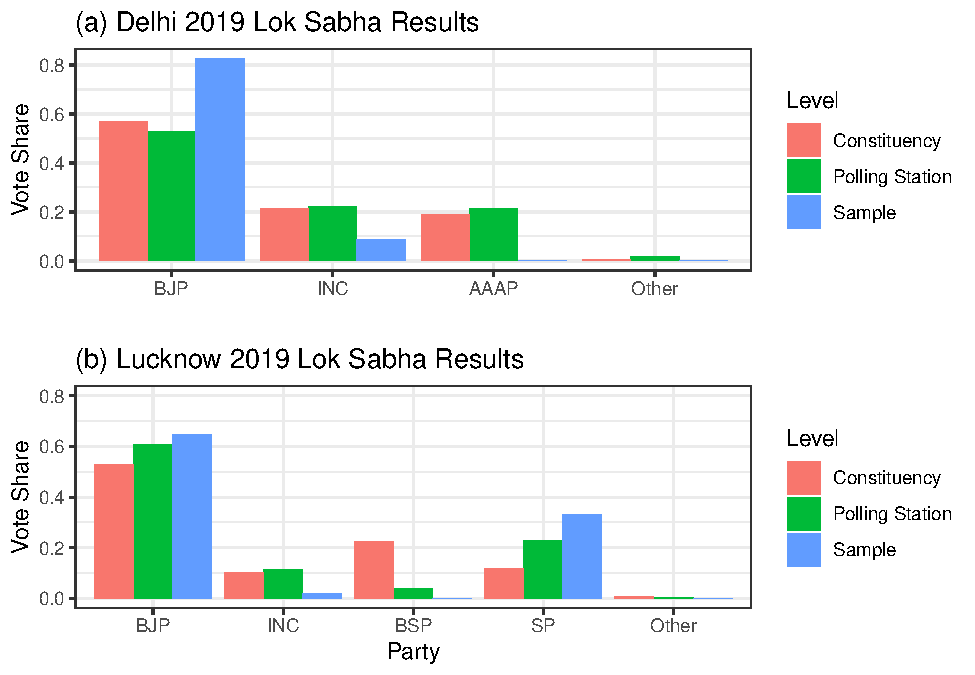
\includegraphics{supplementary-information_files/figure-latex/unnamed-chunk-62-1.pdf}
\caption{\label{fig:party_vote_comparison}{[}Exploratory{]} Comparison
of the distributions of party-wise support between migrants in the
experimental sample and the final vote tallied at the constituency and
polling-station levels.}
\end{figure}

\clearpage

\hypertarget{t2-additional-results}{%
\section{T2 additional results}\label{t2-additional-results}}

\hypertarget{t2-effects-on-trust-and-integration}{%
\subsection{T2 effects on trust and
integration}\label{t2-effects-on-trust-and-integration}}

\begin{table}[!htbp] \centering 
  \caption{[Exploratory] Estimates of T2 effects on trust in political institutions and social integration. Outcomes are whether respondent has trust in the national (1), state (2), and municipal governments (3), and in political parties (4); whether the respondent considers the city to be “home” (5); for how many more years they plan to live in the city (6); and whether they would recommend to friends and relatives in their hometown to come to the city to live and work (7). Weighted least squares estimates of intent to treat effects. Clusters weighted equally. Models include block fixed effects but no additional covariates. Cluster-robust standard errors in parentheses.} 
  \label{} 
\fontsize{10pt}{10pt}\selectfont
\begin{tabular}{@{\extracolsep{5pt}}lccccccc} 
\\[-1.8ex]\hline 
\hline \\[-1.8ex] 
 & \multicolumn{7}{c}{\textit{Dependent variable:}} \\ 
\cline{2-8} 
\\[-1.8ex] & \shortstack{Trust: \\ National \\ Gov.} & \shortstack{Trust: \\ State \\ Gov.} & \shortstack{Trust: \\ Municipal \\ Gov.} & \shortstack{Trust: \\ Political \\ Parties} & \shortstack{Considers \\ City \\ Home} & \shortstack{Plans \\ to Live \\ in City} & \shortstack{Recommends \\ Others Live \\ in City} \\ 
\\[-1.8ex] & (1) & (2) & (3) & (4) & (5) & (6) & (7)\\ 
\hline \\[-1.8ex] 
 T2 & $-$0.001 & 0.050$^{*}$ & 0.043 & $-$0.033 & 0.017$^{**}$ & 0.677 & 0.007 \\ 
  & (0.023) & (0.026) & (0.029) & (0.026) & (0.007) & (3.344) & (0.030) \\ 
 \hline \\[-1.8ex] 
Observations & 1,969 & 1,969 & 1,969 & 1,969 & 1,969 & 1,969 & 1,969 \\ 
Adjusted R$^{2}$ & 0.016 & 0.034 & 0.015 & 0.009 & 0.004 & 0.020 & 0.001 \\ 
\hline 
\hline \\[-1.8ex] 
\multicolumn{8}{r}{$^{*}$p$<$0.1; $^{**}$p$<$0.05; $^{***}$p$<$0.01} \\ 
\end{tabular} 
\end{table}

\clearpage

\hypertarget{t2-results-without-covariates}{%
\subsection{T2 results without
covariates}\label{t2-results-without-covariates}}

\begin{table}[!h]

\caption{\label{tab:unnamed-chunk-64}[Exploratory] T2 experimental results for exposure to campaigning during the 2019 elections. Weighted least squares estimates of intent to treat effects. Clusters weighted equally. Models do not include covariates. Cluster-robust standard errors in parentheses.}
\centering
\fontsize{10}{12}\selectfont
\begin{tabular}[t]{lcccccc}
\toprule
\multicolumn{1}{c}{} & \multicolumn{1}{c}{ } & \multicolumn{5}{c}{Index Components} \\
\cmidrule(l{3pt}r{3pt}){3-7}
 & \makecell[c]{Campaigning\\ Exposure\\ Index \\(1)} & \makecell[c]{Basti\\Visits by\\ Politicians \\(2)} & \makecell[c]{Home Visit\\ by Politician or\\ Party Worker  \\(3)} & \makecell[c]{Number\\ of\\ Gifts \\(4)} & \makecell[c]{Migrant-\\ Focused\\ Campaigning \\(5)} & \makecell[c]{Perceived\\ Campaign\\ Intensity \\(6)}\\
\midrule
T2 treatment & 0.101 & 0.055 & 0.039 & 0.020 & 0.006 & 0.073\\
 & (0.058) & (0.080) & (0.039) & (0.014) & (0.046) & (0.032)\\
\midrule
p-value (upper) & 0.043 & 0.249 & 0.160 & 0.078 & 0.445 & 0.012\\
Control mean & -0.039 & 0.559 & 0.550 & 0.013 & 0.425 & 0.676\\
Observations & 1,969 & 1,969 & 1,969 & 1,969 & 1,969 & 1,931\\
No. of Clusters & 87 & 87 & 87 & 87 & 87 & 87\\
Adjusted $R^2$ & 0.056 & 0.049 & 0.033 & 0.012 & 0.004 & 0.012\\
DV values & $[-0.96, 3.65]$ & $\{0, \ldots, 4\}$ & $\{0, 1\}$ & $\{0, 1, 2\}$ & $\{0, 1\}$ & $\{0, 0.33, 0.67, 1\}$\\
\bottomrule
\end{tabular}
\end{table}

\clearpage

\hypertarget{migrant-voting-behavior-over-time}{%
\section{Migrant voting behavior over
time}\label{migrant-voting-behavior-over-time}}

\begingroup\fontsize{9}{11}\selectfont

\begin{longtable}[t]{>{\raggedright\arraybackslash}p{20em}>{\raggedright\arraybackslash}p{20em}}
\caption{\label{tab:unnamed-chunk-65}\label{tab:voting_behavior}Migrant versus non-migrant voting behavior in Delhi elections over time. Note, in some cases the reported percentages represent weighted averages based on relative population shares described in the given source.}\\
\toprule
Election & Vote choice\\
\midrule
\endfirsthead
\caption[]{(\textit{continued}) Migrant versus non-migrant voting behavior in Delhi elections over time.}\\
\toprule
Election & Vote choice\\
\midrule
\endhead

\endfoot
\bottomrule
\endlastfoot
\cellcolor{gray!6}{\textbf{2020 Vidhan Sabha Elections}  \newline \newline Source: Lokniti Pre-Poll Election Survey 2020 bit.ly/35FG4ei} & \cellcolor{gray!6}{\textbullet INC:  \newline \hspace*{2em}\textbullet Migrants: 4\% \newline \hspace*{2em}\textbullet Non-migrants: 5\% \newline \textbullet BJP: \newline \hspace*{2em}\textbullet Migrants: 43\% \newline \hspace*{2em}\textbullet Non-migrants: 38\% \newline \textbullet AAP: \newline \hspace*{2em}\textbullet Migrants: 51\% \newline \hspace*{2em}\textbullet Non-migrants: 55\% \newline \textbullet Others: \newline \hspace*{2em}\textbullet Migrants: 3\% \newline \hspace*{2em}\textbullet Non-migrants: 2\%}\\
\textbf{2015 Vidhan Sabha Elections}  \newline \newline Source: Lokniti Post-Poll Election Survey 2015 bit.ly/35FG4ei & \textbullet INC:  \newline \hspace*{2em}\textbullet Migrants: 8\% \newline \hspace*{2em}\textbullet Non-migrants: 10\% \newline \textbullet BJP: \newline \hspace*{2em}\textbullet Migrants: 33\% \newline \hspace*{2em}\textbullet Non-migrants: 32\% \newline \textbullet AAP: \newline \hspace*{2em}\textbullet Migrants: 55\% \newline \hspace*{2em}\textbullet Non-migrants: 55\% \newline \textbullet Others: \newline \hspace*{2em}\textbullet Migrants: 3\% \newline \hspace*{2em}\textbullet Non-migrants: 3\%\\
\cellcolor{gray!6}{\textbf{2008 Vidhan Sabha Elections}  \newline \newline Kumar, Sanjay. 2013. \textit{Changing Electoral Politics in Delhi: From Caste to Class.} SAGE Publications India. p. 81. \newline \newline Vote choice comparisons between constituencies dominated by migrants from UP/Bihar and constituencies not dominated by such migrants (“Rest”)} & \cellcolor{gray!6}{\textbullet INC:  \newline \hspace*{2em}\textbullet Migrant constituencies: 36\% \newline \hspace*{2em}\textbullet Rest: 44\% \newline \textbullet BJP: \newline \hspace*{2em}\textbullet Migrant constituencies: 34\% \newline \hspace*{2em}\textbullet Rest: 37\% \newline \textbullet BSP: \newline \hspace*{2em}\textbullet Migrant constituencies: 19\% \newline \hspace*{2em}\textbullet Rest: 12\% \newline \textbullet Others: \newline \hspace*{2em}\textbullet Migrant constituencies: 11\% \newline \hspace*{2em}\textbullet Rest: 6\%}\\*
\end{longtable}
\endgroup{}

\clearpage

\hypertarget{research-locations}{%
\section{Research locations}\label{research-locations}}

\begin{figure}

{\centering 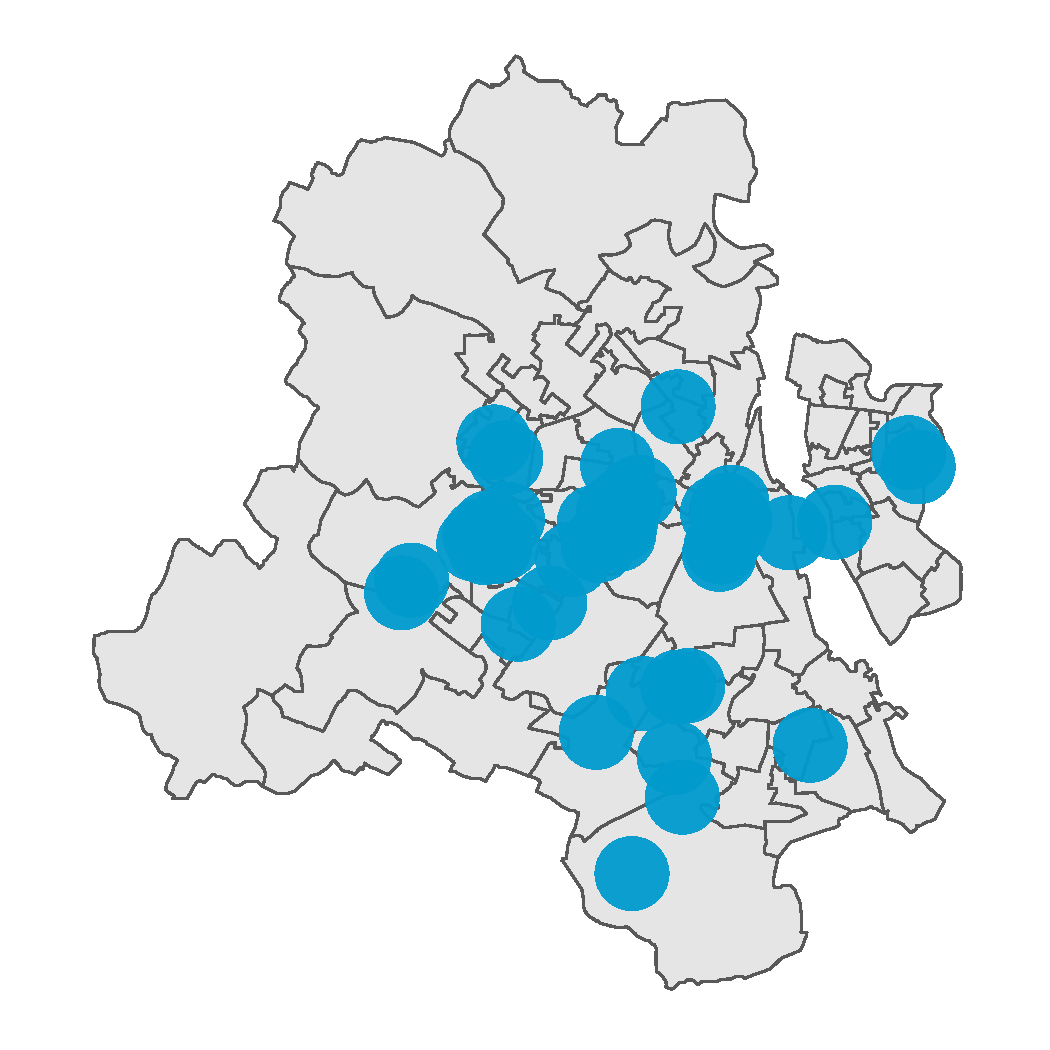
\includegraphics[width=0.5\linewidth]{pic-del-map} 

}

\caption{Approximate locations of the experimental sample: Delhi. Boundaries represent assembly constituency segments within the Lok Sabha constituencies in which the experiment was fielded.}\label{fig:unnamed-chunk-66}
\end{figure}

\clearpage

\begin{figure}

{\centering 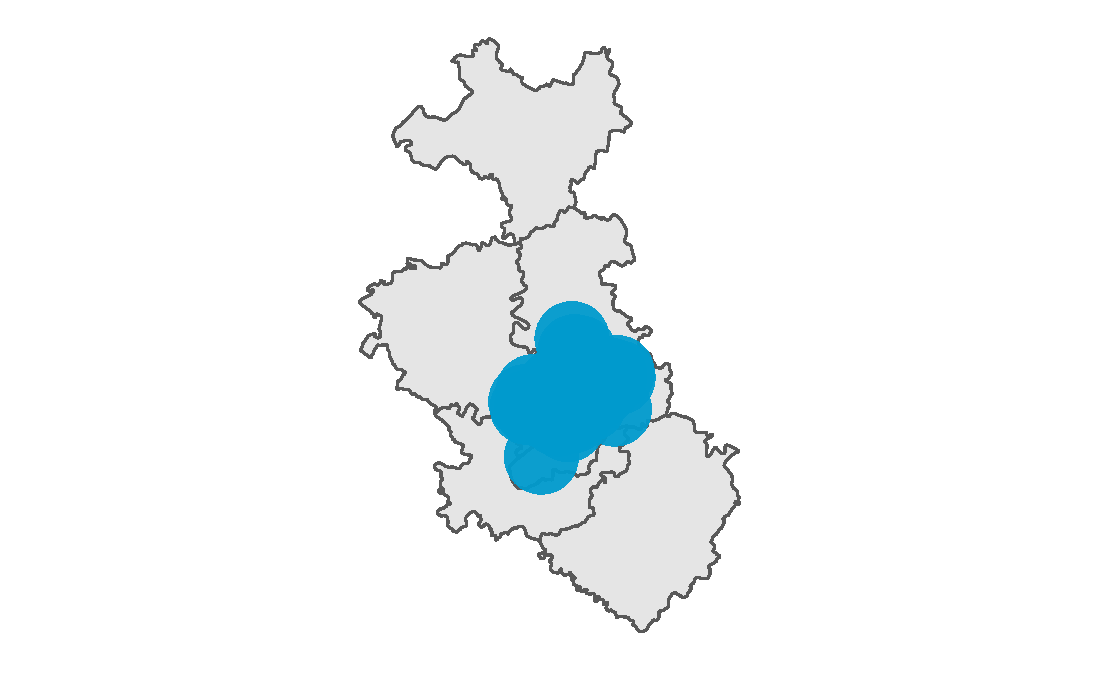
\includegraphics[width=0.8\linewidth]{pic-luc-map} 

}

\caption{Approximate locations of the experimental sample: Lucknow. Boundaries represent assembly constituency segments within the Lok Sabha constituencies in which the experiment was fielded.}\label{fig:unnamed-chunk-67}
\end{figure}

\end{document}
